% SN2018.tex
% Darja Maljceva, Vladimir Batagelj
% Analysis of the social networks literature
% ----------------------------------------------------------------------------
% version 0: March 2017
% ----------------------------------------------------------------------------
% https://github.com/bavla/SocNet
% C:\Users\batagelj\work\Python\WoS\SocNet\2018
% ----------------------------------------------------------------------------
\documentclass[hyperref={pdfstartview={FitBH -32768},
                         pdfpagemode=FullScreen,
                         plainpages=false,
                         colorlinks=true}
              ]{beamer}
%\usepackage[slovene]{babel}
%\usepackage[cp1250]{inputenc}
\usepackage[utf8]{inputenc}
\usepackage{latexsym}
\usepackage{amsfonts}
\usepackage{crayola}
%\usepackage{datum}
\usepackage{xspace}

% Antibes, Berkeley, Berlin,
% Dresden, Frankfurt,
% Madrid, Malmoe, Marburg,
% PaloAlto, Pittsburgh, Szeged, Warsaw
\usetheme{Malmoe}
% default, infolines, miniframes, shadow, sidebar, smoothbars,
% smoothtree, split, tree
\useoutertheme{sidebar}
% albatross, beetle, crane, default, dolphin, dove, fly, lily, orchid, rose
% seagull, seahorse, sidebartab, structure, whale
\usecolortheme{dove}
\useinnertheme{circles}
% default, professionalfonts, serif, structurebold,
% structureitalicserif, structuresmallcapsserif
\usefonttheme{default}

% title page --------------------------------------------------------------
% \pgfdeclareimage[width=7.8mm]{uniLJ}{../../../2014/barcelona/slides/pics/logoUL.pdf}
\pgfdeclareimage[width=16mm]{imfm}{./pics/imfm.png}
\setbeamercolor*{logo}{fg=red,bg=white}
\logo{\pgfuseimage{imfm}}
%\title[Bikes]{\textbf{Bikes }}\subtitle{data}
\title[SNA. Bibliographic Network Analysis]{\textbf{Social Network Analysis:}}\subtitle{Bibliographic Network Analysis of the Field and its Evolution}
\author[D. Maltseva, V. Batagelj]{Daria Maltseva, Vladimir Batagelj} 
\institute[IMFM \& IAM UP]{IMFM Ljubljana, IAM UP Koper and NRU HSE Moscow }
\date[November 21, 2018]{\small
\textcolor{BrickRed}{\textbf{Sredin Seminar 1282}} \\
November 21, 2018}
\normalsize



% user's macros ----------------------------------------------------------
\newcommand{\Pajek}{\texttt{\textbf{Pajek}}\xspace}
\newcommand{\WoSPajek}{\texttt{\textbf{WoS2Pajek}}\xspace}
%\newcommand{\Pajek}{Pajek}
\newcommand{\keyw}[1]{\textcolor{red}{\emph{#1}}}
\newcommand{\important}[1]{\textcolor{NavyBlue}{#1}}
\newcommand{\RR}{\Bbb{R}}
\newcommand{\NN}{\Bbb{N}}
\newcommand{\ZZ}{\Bbb{Z}}
\newcommand{\QQ}{\Bbb{Q}}
\newcommand{\network}[1]{\mathcal{#1}}
\newcommand{\vertices}[1]{\mathcal{#1}}
\newcommand{\edges}[1]{\mathcal{#1}}
\newcommand{\arcs}[1]{\mathcal{#1}}
\newcommand{\Net}{\network{N}}
\newcommand{\argmin}{\mathop{\mbox{argmin}}\nolimits}
\newcommand{\relation}[1]{\textbf{\emph{$\_\!\_$~#1~$\_\!\_$\,}}}
\newcommand{\functions}[1]{\mathcal{#1}}
\newcommand{\define}[1]{\emph{\textcolor{red}{#1}}}
\newcommand{\card}[1]{\mbox{card}(#1)}
\newcommand{\URL}[1]{{\footnotesize\texttt{#1}}}
\newcommand{\tita}[1]{\textit{#1}}      % italic
\newcommand{\cling}{\mathbf{C}}
\newcommand{\unitX}{\mbox{X}}
\newcommand{\unitY}{\mbox{Y}}
\newcommand{\unitZ}{\mbox{Z}}
\newcommand{\outdeg}{\mbox{outdeg}}
\newcommand{\indeg}{\mbox{indeg}}
\newcommand{\ato}{\mathrel{:=}}
\newcommand{\unit}{\mbox{X}}
\newcommand{\Units}{\vertices{U}}
\def\Min{\mathop{\mbox{Min}}\nolimits}
\def\Max{\mathop{\mbox{Max}}\nolimits}
\newcommand{\graph}[1]{\mathcal{#1}}
\newcommand{\function}[3]{#1\,{:}\ #2\to#3}
\newcommand{\Gph}{\network{G}}
\newcommand{\GphH}{\network{H}}
\newcommand{\Graph}{\mathbf{G}}
\newcommand{\tit}[1]{\textit{#1}}      % italic
\newcommand{\diag}{\mbox{diag}}
\newcommand{\func}[1]{\textit{#1}}
\newcommand{\Relation}[1]{\mathbf{#1}}
\newcommand{\Time}{\mathcal{T}}
%\newcommand{\cmdkey}{\raisebox{-.035em}{\includegraphics[height=.75em]{command.pdf}}}
\newcommand{\cmdkey}{\raisebox{-.025em}{\includegraphics[height=.7em]{command.pdf}}}
\newcommand{\Mw}{\mathop{\raisebox{-1.5pt}{\mbox{$\Box$\kern-.55em\raisebox{2.5pt}{{\tiny $r$}}\kern2.9pt}}}}
\newcommand{\Mv}{\mathop{\raisebox{-1.5pt}{\mbox{$\Box$\kern-.55em\raisebox{2.5pt}{{\tiny $h$}}\kern2.9pt}}}}
\newcommand{\Ct}{\mathbf{Ct}}
\newcommand{\N}{\mathbf{N}}
\newcommand{\WA}{\mathbf{W\!A}}

\newcommand{\clock}{\count254=\time \divide\count254 by 60
 \count255=\count254 \multiply\count255 by -60
 \advance\count255 by \time
 \ifnum\count254<10 0\fi\number\count254\,:\,%
 \ifnum\count255<10 0\fi\number\count255}


%\newcommand{\diag}{\mathop{\rm diag}\nolimits}

%\graphicspath{{./pics/}}
\graphicspath{{./pics/}}

%******************************************************************************
\begin{document}

\hypersetup{pdfauthor={D. Maltseva, V. Batagelj}}
%\hypersetup{pdftitle={Bikes; 1. data}}
\hypersetup{pdftitle={SNA. Evolution of the field}}

\frame{\maketitle}

\begin{frame}
\frametitle{Outline}
\small
\begin{enumerate}
\item Introduction 
\item Data collection 
\item Networks construction 
\item Statistics on networks
\item Works citations through time
\item Collaboration among authors
\item Citation among authors / journals
\item Co-citation among authors / journals
\item Keywords co-occurence
\end{enumerate}

%\parbox{44mm}{\tableofcontents}
%\parbox{56mm}{\centerline{\includegraphics[width=40mm]{Davis1.jpg}}
% \includegraphics[width=56mm]{Davis2.jpg}
%}
%\bigskip

%\scriptsize
%\textbf{Vladimir Batagelj}: \href{mailto:vladimir.batagelj@fmf.uni-lj.si}%
%       {\texttt{vladimir.batagelj@fmf.uni-lj.si}}\medskip
%\textbf{Selena Praprotnik}: \href{mailto:selena.praprotnik@fmf.uni-lj.si}%
%       {\texttt{selena.praprotnik@fmf.uni-lj.si}}

%\textbf{Version (\today, \clock):}
%\href{http://vladowiki.fmf.uni-lj.si/lib/exe/fetch.php?media=pub:pdf:sreda1273.pdf}{sreda1273.pdf}

\end{frame}

\section{Introduction}

%******************************************************************************
\begin{frame}[fragile]
\frametitle{Inroduction}
\small

Social Network Analysis (SNA) has moved from a fragmented direction represented by the works of individual scientific groups unrelated to each other, to a discipline whose representatives by 1990 have formed an “invisible college” and achieved the status of  what Kuhn had labeled a “normal science” [Freeman, 2004; Hummon and Carley, 1993]. \medskip

Starting from that time, the field has grown significantly, which can be seen by the number of scientific publications [Otte and Rousseau, 2002] in different scientific fields, including Natural Sciences, which lead to the so called “physicists` invasion” into SNA [Batagelj et al., 2014] and resulted with the development of Network Science discipline. \medskip

This calls into a question whether the field remains unified and which scientific groups (by disciplines, thematic agenda, etc.) it is currently formed of. Thus, the aim of the current study is to trace the evolution of the field of Social Network Analysis using bibliographic approach.  \medskip 

\end{frame}


\begin{frame}[fragile]
\frametitle{Previous studies}
\tiny
\begin{enumerate}

\item Hummon N.P., Doreian P., Freeman L.C. (1990). Analyzing the Structure of the Centrality-Productivity Literature Created Between 1948 and 1979 / Science Communication. 11, 4, 459 – 480. 

\item   Freeman, L. (2004). The development of social network analysis. A Study in the Sociology of Science, 1.

\item  Hummon, N. P., Carley, K. (1993). Social networks as normal science. Social networks, 15(1), 71-106.

\item   Otte, E., Rousseau, R. (2002). Social network analysis: a powerful strategy, also for the information sciences. Journal of information Science, 28(6), 441-453. 

\item Borgatti, S. P., Foster, P. C. (2003). The network paradigm in organizational research: A review and typology. Journal of management, 29(6), 991-1013.

\item Leydesdorff L., Schank T., Scharnhorst A., De Nooy W. (2008). Animating the development of Social Networks over time using a dynamic extension of multidimensional scaling / El Profesional de Informacion, 17(6).

\item Lazer, D., Mergel, I., and Friedman, A. (2009). Co-citation of prominent social network articles in sociology journals: The evolving canon. Connections, 29(1):43:64. 

\item Brandes, U., Pich, C. (2011). Explorative visualization of citation patterns in social network research. Journal of social structure, 12(8), 1-19.

\item Varga, A. V., Nemeslaki, A. (2012) Do organizational network studies constitute a cohesive communicative field? Mapping the citation context of organizational network research. Journal of Sociology and Social Anthropology, 5(64), XV, 349-364. \

\item Batagelj, V., Doreian P., V., Ferligoj, A., Kejžar N. (2014). Understanding Large Temporal Networks and Spatial Networks: Exploration, Pattern Searching, Visualization and Network Evolution. 

\item Groenewegen, P., Hellsten, I., Leydesdorff, L. (2015) Social Networks as a looking glass on the social networks community. International Sunbelt XXXV Conference. Hilton Metropole, Brighton, UK, June 23 – 28, 2015. Abstracts, 118. 

\end{enumerate}
\end{frame}

\subsection{Data}

%******************************************************************************
\begin{frame}[fragile]
\frametitle{WoS}
\small

To the Web of Science (WoS), Clarivate Analytics’s multidisciplinary databases of bibliographic
information, we put the query
\begin{verbatim} 
"social network*"
\end{verbatim}
Additionally, all the articles from the following journals were collected:
\begin{verbatim}
Social Networks, Network Science, 
Social Network Analysis and Mining, 
Journal of Complex Networks
\end{verbatim}

Other network-related journals \keyw{are not presented} in WoS: 
\begin{verbatim}
Computational Social Networks, Applied Network Science, 
Online Social Networks and Media, Connections, 
Journal of Social Structure
\end{verbatim}

We limited the search to the Web of Science Core Collection because for other data bases from WoS the CR-fields (containing citation information) can not be exported. The first data set was collected in 2007, second -- in June, 2018. 

\end{frame}

\begin{frame}[fragile]
\frametitle{WoS record}
\renewcommand{\baselinestretch}{0.8}
\tiny
\begin{verbatim}
PT J
AU GRANOVET.MS
TI STRENGTH OF WEAK TIES
SO AMERICAN JOURNAL OF SOCIOLOGY
LA English
DT Article
C1 JOHNS HOPKINS UNIV, BALTIMORE, MD 21218 USA.
CR BARNES JA, 1969, SOCIAL NETWORKS URBA
   BECKER MH, 1970, AM SOCIOL REV, V35, P267
   BERSCHEID E, 1969, INTERPERSONAL ATTRAC
   BOISSEVAIN J, 1968, MAN, V3, P542
   BOTT E, 1957, FAMILY SOCIAL NETWOR
NR 61
TC 2156
PU UNIV CHICAGO PRESS
PI CHICAGO
PA 5720 S WOODLAWN AVE, CHICAGO, IL 60637
SN 0002-9602
J9 AMER J SOCIOL
JI Am. J. Sociol.
PY 1973
VL 78
IS 6
BP 1360
EP 1380
PG 21
SC Sociology
GA P7726
UT ISI:A1973P772600003
ER
SK IP
\end{verbatim}
\end{frame}

\begin{frame}[fragile]
\frametitle{WoS}
\small
We call a \keyw{terminal} node  a node without a description in the collected data set -- it appears only in the WoS CR field as a reference. \medskip

We additionally collected on WoS and Google data for terminal nodes with large indegree in the citation network -- highly cited works without description in the collected data set. If a description of a node was not available in WoS we manually constructed a corresponding description without CR data (using RIS biblographic format and converting it to WoS).\medskip

As the data set of 2007 was already completed, we made this additional search only for works 2008-* in July 2018. 
\end{frame}

\subsection{Networks}

%******************************************************************************

\begin{frame}[fragile]
\frametitle{Types of networks and partitions}
\small
We applied the WoS2Pajek 1.5  to the collected data.\medskip

The following networks were constructed: 
\begin{enumerate}
\item the authorship network $WA$ on works $\times$ authors  (from the field AU), 
\item the journalship network $WJ$ on  works $\times$ journals  (from the field CR or J9), 
\item the keywordship network $WK$ on works  $\times$ keywords (from the field ID or DE or TI), 
\item the citation network $Cite$ on works (from the field CR).
\end{enumerate}

We obtained also the following partitions: 
\begin{enumerate}
\item the partition $year$ of works by publication year, 
\item the $DC$ partition distinguishing between works with complete description (DC=1) and the cited only works (DC=0),
\item the vector of number of pages $NP$.
\end{enumerate}
\end{frame}

\begin{frame}[fragile]
\frametitle{ISI names}
\footnotesize
The usual \keyw{ISI name} of a work (field CR)
\begin{verbatim}
GRANOVETTER M, 1985, AM J SOCIOL, V91, P481
\end{verbatim}
has the following structure\medskip

   AU \texttt{+ ', ' +} PY \texttt{+ ', ' +} SO[:20] \texttt{+ ', V' +} VL  \texttt{+ ', P' +} BP\medskip

\noindent All its elements are in upper case.

In WoS the same work can have different ISI names. To improve
the precission the program \WoSPajek supports also
\keyw{short names} (similar to the names used in HISTCITE output).
They have the format:\medskip

   LastNm[:8] \texttt{+ '\_' +} FirstNm[0] \texttt{+ '(' +} PY
   \texttt{+ ')' +} VL \texttt{+ ':' +} BP\medskip

For example: \quad
\texttt{GRANOVET\_M(1985)91:481}

From the last names with prefixes \texttt{VAN}, \texttt{DE}, \ldots the space is deleted.
Unusual names start with character \texttt{*} or \texttt{\$}.

\end{frame}

\begin{frame}[fragile]
\frametitle{Equivalent works, authors and journals}
\footnotesize

\begin{verbatim}
BOYD_D(2007)13 | BOYD_D(2008)13:210
GRANOVET_M(1973)78:1360 | GRANOVET_M(1973)78:6
COLEMAN_J(1988)94:95 | COLEMAN_J(1988)94:S95
\end{verbatim}

\begin{verbatim}
GRANOVET_M
GRANOVET_
\end{verbatim}

\begin{verbatim}
63656		1312696	10849	SONEANMI	| SOCIAL NETWORK ANAL
63657		1330776	3	SONEANMI	| SOCIAL NETWORKS ANAL
63658		1311789	645	SONEANMI	| SOC NETW ANAL MIN
63659		1313366	7	SONEANMI	| SOCIAL NETW ANAL MIN
63660		1315722	7	SONEANMI	| SOC NETW ANAL MINING
...
55366		1351847	54714		1	PSPOSC 	| PS POLITICAL SCIENCE
55768		1320199	23066		5	POSC		| POLITICAL SCI
55769		1320573	23440		3	POSC		| POLIT SCI
56082		1297982	849		224	PSSCPO	| PS-POLIT SCI POLIT
56083		1298064	931		110	PSSCPO	| PS-POLITICAL SCI POL
\end{verbatim}
\end{frame}

\begin{frame}[fragile]
\frametitle{Equivalent works, authors and journals}
\footnotesize

There are two possibilities how to correct the data:
\begin{itemize}
\item to make corrections in the local copy of original data (WoS file);
\item to make the equivalence partition of nodes and shrink the set of works accordingly in all  obtained networks.
\end{itemize}

For the \textbf{works} with largest counts we prepared lists of possible equivalents and manually determined equivalence classes. With a program in R we produced a Pajek's partition $EQ.clu$ file used for shrinking the set of works. Using the partition $p=worksEQ$, we shrink using Pajek the Citation network $cite$, $WA$, $WJ$, and $WK$. We had to shrink also partitions $year$,  $DC$ and the vector $NP$. \smallskip 


The total cleaning of \textbf{journals} would require too much time. We decided to clean only the high frequency elements (cited 200 times and more) and consider bugs in low frequency elements as a noise. We got the list $journalK100.csv$ with 3714 titles for inspection.\smallskip  

We also produced a list of frequent journal names (of length at most 5), have chosen all the cases that could be regarded as abbreviations (\textit{CACM, JACM, JASA}), and manually searched for them. 

\end{frame}

\begin{frame}[fragile]
\frametitle{Sizes of Original cleaned and Reduced networks}
\small 

\begin{center}
\begin{tabular}{c|r|r|r|r}
	&\# nodes (sum)	& \# nodes 1	&\# nodes 2	& \# arcs \\ \hline		 
CiteN & 1,297,133 & & & 2,753,633\\ 
\textbf{CiteR} & \textbf{70,792} & & & 398,199 \\ \hline
WAn	& 1,693,104	& 1,297,133	& 395,971	& 1,442,240 \\ 	
\textbf{WAr}	& 163,803	& \textbf{70,792}	& \textbf{93,011}	& 215,901 \\ \hline
WKn &  	1,329,542	& 1,297,133	& 32,409	& 1,167,670 \\  
\textbf{WKr}	& 103,201	& \textbf{70,792}	& \textbf{32,409}	& 1,167,666 \\ \hline
WJn & 	1,366,279	& 1,297,133	& 69,146	& 720,044    \\ 	
\textbf{WJr} 	& 79,735	& \textbf{70,792}	& \textbf{8,943}	& 61,741 \\ \hline
\end{tabular}				
\end{center}		

An important property of all these networks is that they share as the first node set the same set of works (papers, reports, books, etc.) -- they are \keyw{linked}.
\end{frame}

\section{Static}
\subsection{Statistics}

%******************************************************************************\

\begin{frame}[fragile]
\frametitle{Cite network\label{maxinc}\\ \normalsize Distribution of works by years}

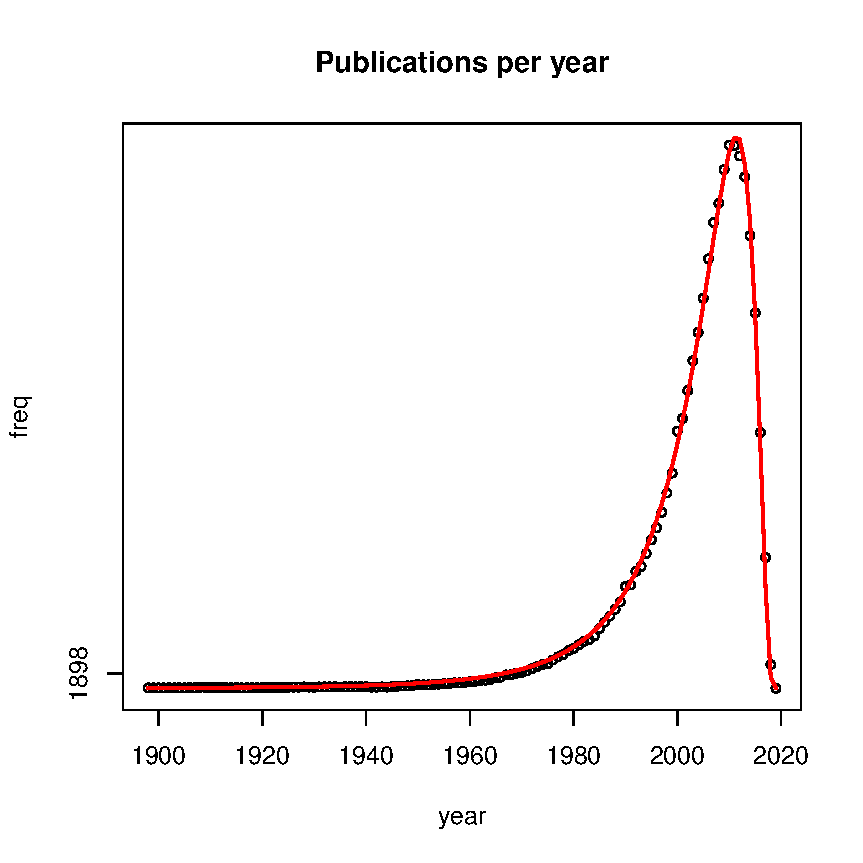
\includegraphics[width=50mm]{pubYear.pdf}
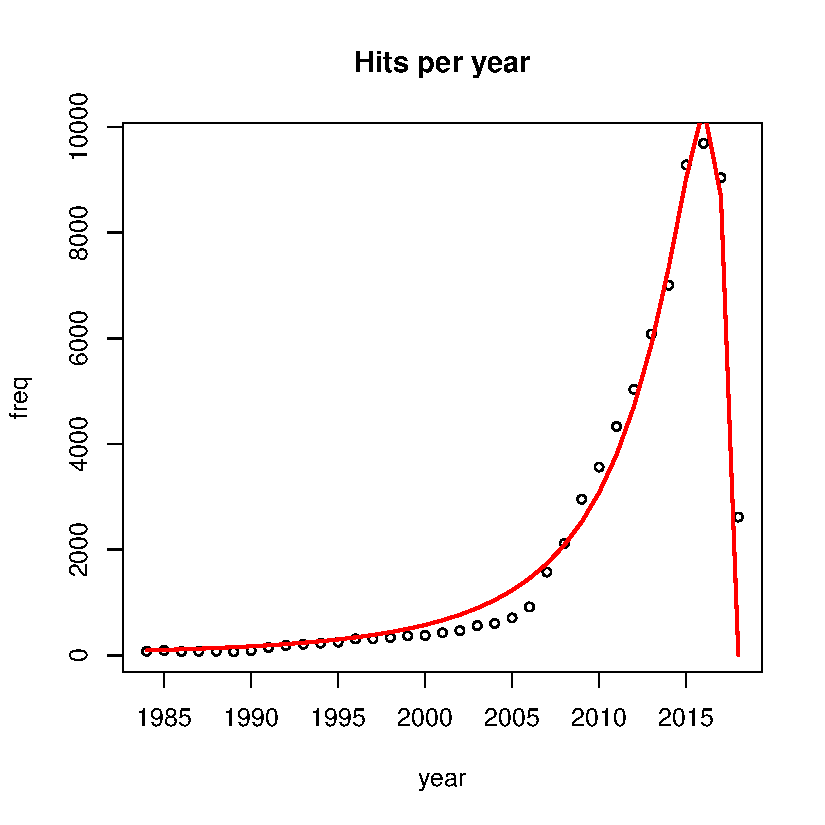
\includegraphics[width=50mm]{yearshits7.pdf}

\small
The distributions fits the \keyw{log norma}l distribution 

\footnotesize
$c\cdot \mbox{dlnorm}(2019-year,a,b)$, where $a = 2.543$, $b = 0.7206$, and $c = 1.278 10^6$. \medskip

$c\cdot \mbox{dlnorm}(2018-year,a,b)$, where $a = 1.501$, $b = 0.9587$, and $c = 7.110 10^4$.\medskip

\end{frame}

\begin{frame}[fragile]
\frametitle{Cite network\label{maxind}\\ \normalsize Indegree distribution}

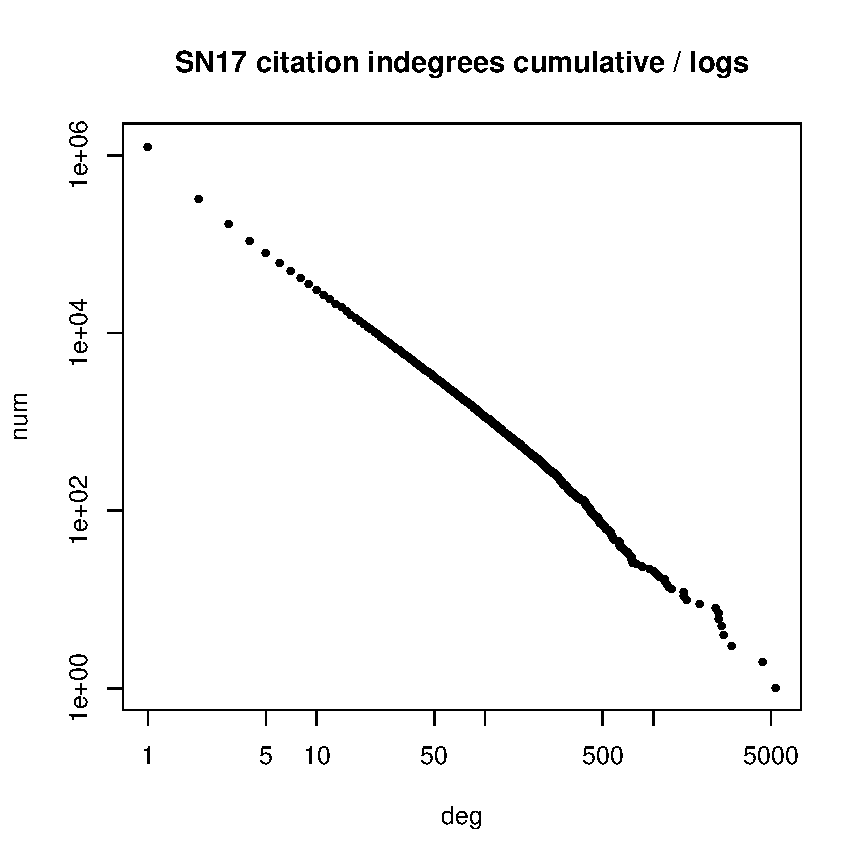
\includegraphics[width=50mm]{CiteIndegCum.pdf}
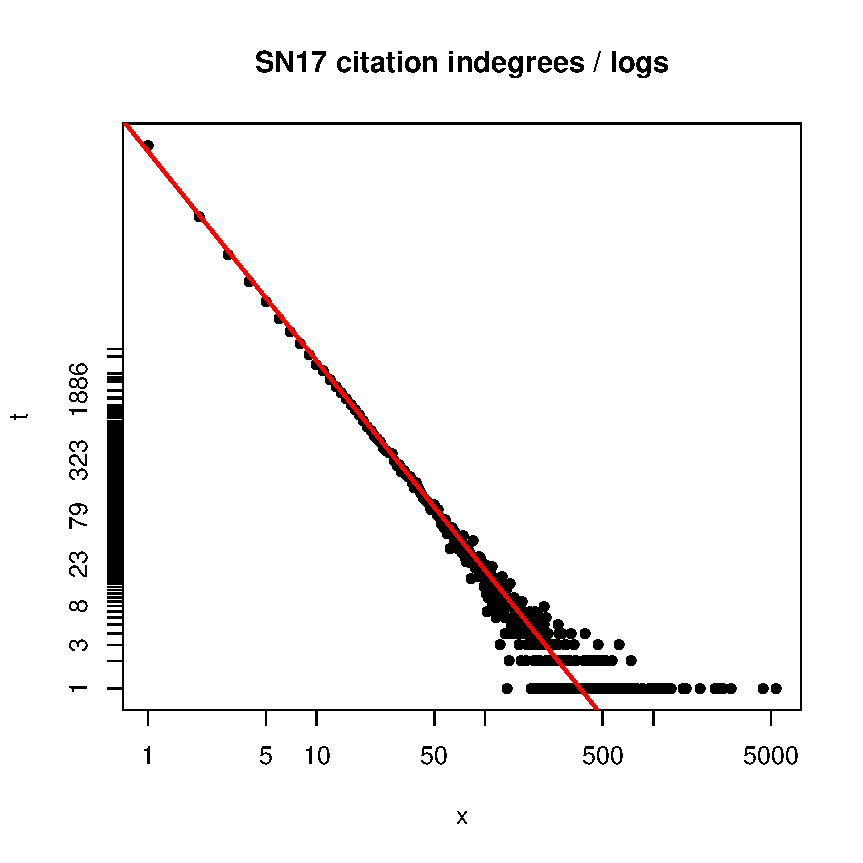
\includegraphics[width=50mm]{CiteIndegplfit.pdf}

\small
The indegree distribution in citation network follows the \keyw{power law} $f = c \cdot n^{-\alpha}$.

Fitted $\alpha = 2.3007$, $c=749338$.
\end{frame}

\begin{frame}[fragile]
\frametitle{Cite net\label{maxine}\\ \normalsize The most cited works - indegree}

\renewcommand{\arraystretch}{0.82}
\tiny
\begin{tabular}{r|r|l||r|r|l}
i	& freq	& id	                                           & i	& freq & id \\ \hline
1& 	5348& 	\textbf{WASSERMA\_S(1994):} & 	31& 	734& 	*NEWMAN\_M(2001)98:404	\\
2& 	4471& 	\textbf{GRANOVET\_M(1973)78:1360} & 	32& 	719& 	*NEWMAN\_M(2010):	\\
3& 	2906& 	*WATTS\_D(1998)393:440& 	33& 	701& 	PORTES\_A(1998)24:1	\\
4& 	2614& 	*BARABASI\_A(1999)286:509& 	34& 	687& 	BLEI\_D(2003)3:993	\\
5& 	2561& 	\textbf{FREEMAN\_L(1979)1:215}& 	35& 	670& 	\textbf{BURT\_R(2004)110:349}	\\
6& 	2447& 	BOYD\_D(2007)13:210& 	36& 	654& 	HANSEN\_M(1999)44:82	\\
7& 	2429& 	MCPHERSO\_M(2001)27:415& 	37& 	639& 	PALLA\_G(2005)435:814	\\
8& 	2330& 	\textbf{BURT\_R(1992):}& 	38& 	634& 	*CLAUSET\_A(2004)70:066111	\\
9& 	1886& 	\textbf{COLEMAN\_J(1988)94:95}& 	39& 	629& 	*BONACICH\_P(1987)92:1170	\\
10& 	1572& 	*NEWMAN\_M(2003)45:167& 	40& 	628& 	ERDOS\_P(1959)6:290	\\
11& 	1520& 	*GIRVAN\_M(2002)99:7821& 	41& 	628& 	UZZI\_B(1997)42:35	\\
12& 	1510& 	\textbf{PUTNAM\_R(2000):}& 	42& 	628& 	\textbf{ROGERS\_E(2003):}	\\
13& 	1285& 	*ALBERT\_R(2002)74:47& 	43& 	613&  \textbf{PUTNAM\_R(1993):}	\\
14& 	1240& 	\textbf{GRANOVET\_M(1985)91:481}& 	44& 	593& 	BERKMAN\_L(1979)109:186	\\
15& 	1192& 	\textbf{SCOTT\_J(2000):}& 	45& 	583& 	\textbf{ZACHARY\_W(1977)33:452}	\\
16& 	1171& 	\textbf{EVERETT\_M(2002):}& 	46& 	572& 	\textbf{BORGATTI\_S(2009)323:892} \\
17& 	1166& 	NEWMAN\_M(2004)69:026113& 	47& 	569& 	*NEWMAN\_M(2001)64:025102	\\
18& 	1093& 	\textbf{COLEMAN\_J(1990):}& 	48& 	565& 	\textbf{BURT\_R(2005):}	\\
19& 	1058& 	STEINFIE\_C(2007)12:1143& 	49& 	561& 	ADLER\_P(2002)27:17	\\
20& 	1034& 	FORTUNAT\_S(2010)486:75& 	50& 	559& 	\textbf{CHRISTAK\_N(2008)358:2249}	\\
21& 	999& 	\textbf{BORGATTI\_S(2002):}& 	51& 	555&  \textbf{ROGERS\_E(1995):}	\\
22& 	945& 	\textbf{CHRISTAK\_N(2007)357:370}& 	52& 	554& 	MILGRAM\_S(1967)1:61	\\
23& 	867& 	\textbf{FREEMAN\_L(1977)40:35}& 	53& 	553& 	BARON\_R(1986)51:1173	\\
24& 	854& 	\textbf{HANNEMAN\_R(2005):}& 	54& 	550& 	\textbf{GRANOVET\_M(1978)83:1420}	\\
25& 	800& 	\textbf{LIN\_N(2001):}& 	55& 	539& 	\textbf{FISCHER\_C(1982):}	\\
26& 	757& 	KAPLAN\_A(2010)53:59& 	56& 	537& 	BRIN\_S(1998)30:107	\\
27& 	756& 	*BLONDEL\_V(2008):P10008& 	57& 	524& 	\textbf{MARSDEN\_P(1990)16:435}	\\
28& 	742& 	NAHAPIET\_J(1998)23:242& 	58& 	523& 	KEMP\_D(2003):137	\\
29& 	740& 	FORNELL\_C(1981)18:39& 	59& 	523& 	KLEINBER\_J(1999)46:604	\\
30& 	740& 	*NEWMAN\_M(2006)103:8577& 	60& 	517& 	*BOCCALET\_S(2006)424:175	\\ \hline
\end{tabular}
Labels ending with $:$ represent books
\end{frame}

\begin{frame}[fragile]
\frametitle{Cite net \label{maxina}\\ \normalsize The most citing work - outdegree}
\small
\renewcommand{\arraystretch}{0.82}
\tiny
\begin{tabular}{r|r|l||r|r|l}
i&	freq& 	id&	i&	freq&	id	\\ \hline 
1& 	1572& 	CHAPMAN\_C(2016):1&	11& 	731& 	TSATSOU\_P(2014):1\\
2& 	1406& 	HRUSCHKA\_D(2010)5:1&	12& 	654& 	GOODALE\_E(2017):IX\\
3& 	1293& 	COWARD\_F(2015):1&	13& 	649& 	PEPPER\_G(2017)40:S0140525X1700190X\\
4& 	1254& 	FITZGERA\_P(2008):1&	14& 	632& 	STROM\_R(2012):1\\
5& 	1207& 	DAVIES\_N(2015):V&	15& 	613& 	SCHACHNE\_G(2015)23:49\\
6& 	1055& 	MARSH\_C(2009):1&	16& 	597& 	\textbf{COSTA\_L(2011)60:329}\\
7& 	942& 	YUS\_F(2011)213:1&	17& 	593& 	\textbf{BRANDES\_U(2005)3418:1}\\
8& 	929& 	\textbf{BOCCALET\_S(2006)424:175}&	18& 	586& 	ROBERTS\_J(2014):1\\
9& 	799& 	REEVES\_M(2017):1&	19& 	557& 	GUNTER\_B(2016):1\\
10& 	768& 	GROSS\_J(2007):1&	20& 	547& 	CASTELLA\_C(2009)81:591\\ \hline 
\end{tabular}

\begin{itemize}
\item MUIJS, D., Reynolds, D.,  CHAPMAN, C. (2015). Educational effectiveness and improvement research and practice: The emergence of the discipline. In The Routledge International Handbook of Educational Effectiveness and Improvement (pp. 33-56). Routledge.
\item  Hruschka, D. J. (2010). Friendship: Development, ecology, and evolution of a relationship (Vol. 5). Univ of California Press.
\item Coward, F., Hosfield, R., Pope, M.,  Wenban-Smith, F. (Eds.). (2015). Settlement, society and cognition in human evolution. Cambridge University Press.
\item Fitzgerald, P.,  Lambkin, B. (2008). Migration in Irish history 1607-2007. Springer.
\item Davies, N.B. Animal Social Networks Foreword. In: Krause, J., James, R., Franks, D. W., Croft, D. P. (Eds.). (2015). Animal social networks. Oxford University Press, USA.
\item Marsh, C. J. (2009). Key concepts for understanding curriculum. Routledge.
\end{itemize}

\end{frame}


\begin{frame}[fragile]
\frametitle{WA net \label{numpap}\\ \normalsize Authors with the largest number of papers - indegree}
\renewcommand{\arraystretch}{0.82}
\tiny
\begin{center}
\begin{tabular}{l|l|l||l|l|l}
Rank& 	Value& 	Id& 	Rank& 	Value& 	Id\\  \hline   
1& 	1169& 	WANG\_Y& 	21& 	552& 	KIM\_H\\ 
2& 	883& 	ZHANG\_Y& 	22& 	550& 	CHEN\_J\\ 
3& 	868& 	CHEN\_Y& 	23& 	536& 	LIU\_X\\ 
4& 	847& 	LI\_Y& 	24& 	533& 	WANG\_L\\ 
5& 	838& 	WANG\_X& 	25& 	509& 	LI\_H\\ 
6& 	819& 	ZHANG\_J& 	26& 	490& 	KIM\_Y\\ 
7& 	788& 	WANG\_J& 	27& 	485& 	ZHANG\_Z\\ 
8& 	786& 	LIU\_Y& 	28& 	474& 	WANG\_Z\\ 
9& 	766& 	LEE\_J& 	29& 	471& 	WANG\_S\\ 
10& 	765& 	LEE\_S& 	30& 	471& 	CHEN\_X\\ 
11& 	749& 	LI\_J& 	31& 	471& 	\textbf{NEWMAN\_M}\\ 
12& 	708& 	LI\_X& 	32& 	462& 	CHEN\_L\\ 
13& 	696& 	CHEN\_C& 	33& 	461& 	ZHANG\_L\\ 
14& 	690& 	KIM\_J& 	34& 	450& 	YANG\_Y\\ 
15& 	620& 	WANG\_H& 	35& 	450& 	ZHANG\_H\\ 
16& 	611& 	ZHANG\_X& 	36& 	432& 	WU\_J\\ 
17& 	611& 	LIU\_J& 	37& 	431& 	LEE\_H\\ 
18& 	570& 	CHEN\_H& 	38& 	420& 	LI\_Z\\ 
19& 	557& 	KIM\_S& 	39& 	420& 	WANG\_W\\ 
20& 	554& 	WANG\_C& 	40& 	417& 	LI\_L\\ \hline  
\end{tabular}
\end{center}

\medskip
\footnotesize
The large number of Chinese authors in the list is a \href{https://en.wikipedia.org/wiki/List_of_common_Chinese_surnames}{"three Zhang, four Li"} effect. It is out of our resources to drill into this. We can only make a warning.
\end{frame}

\begin{frame}[fragile]
\frametitle{WA net \label{numpap}\\ \normalsize Number of authors in works - outdegree}
\renewcommand{\arraystretch}{0.85}
\tiny
\begin{center}
\begin{tabular}{l|l|l||l|l|l}
outdeg&  	Freq&  	Freq\% &  	outdeg&   Freq &	Freq\%\\ \hline   
1*&  	1239496&  	95.5566&  	21&  	4&  	0.0003\\
2&  	18637&  	1.4368&  	22&  	3&  	0.0002\\
3&  	16661&  	1.2844&  	23&  	4&  	0.0003\\
4&  	10617&  	0.8185&  	24&  	2&  	0.0002\\
5&  	5759&  	0.4440&  	25&  	1&  	0.0001\\
6&  	2802&  	0.2160&  	26&  	2&  	0.0002\\
7&  	1322&  	0.1019&  	27&  	5&  	0.0004\\
8&  	686&  	0.0529&  	28&  	2&  	0.0002\\
9&  	384&  	0.0296&  	29&  	1&  	0.0001\\
10&  	247&  	0.0190&  	31&  	3&  	0.0002\\
11&  	155&  	0.0119&  	36&  	1&  	0.0001\\
12&  	90&  	0.0069&  	41&  	1&  	0.0001\\
13&  	70&  	0.0054&  	42&  	1&  	0.0001\\
14&  	54&  	0.0042&  	43&  	1&  	0.0001\\
15&  	32&  	0.0025&  	48&  	1&  	0.0001\\
16&  	12&  	0.0009&  	53&  	1&  	0.0001\\
17&  	14&  	0.0011&  	126&  	1&  	0.0001\\
18&  	9&  	0.0007&  	  & 	 & 	\\
19&  	6&  	0.0005&  	 &	 &	\\
20&  	2&  	0.0002&  	&	 &	\\ \hline
SUM &     &              &       &  1297133 & 100  \\ \hline   
\end{tabular}
\end{center}
* In cited only works only the first author is known. 

\medskip

\footnotesize
Works with the largest number of authors:
\begin{center}
\renewcommand{\arraystretch}{0.82}
\tiny 
\begin{tabular}{l|l|l|l|}
     Rank    & Freq & Id \\ \hline
         1   & 126  & WANG\_M(2016)34:828 \\
         2    & 53   & VASHISHT\_R(2012)7:0039808 \\ 
         3      & 48  & SNIJDERS\_T(2007)170:322 \\ 
         4     & 43  & GUSTAVSS\_A(2011)21:718  \\ 
         5    & 42   & DOLL\_L(1992)29:1 \\ 
         6   &41 &  MAGLIANO\_L(2006)15:219 \\ \hline
\end{tabular}
\end{center}

\end{frame}

\begin{frame}[fragile]
\frametitle{WA net  \\ \normalsize Works with the largest number of authors - outdegree}

Sharing and community curation of mass spectrometry data with Global Natural Products Social Molecular Networking / Nature Biotechnology volume 34, pages 828–837 (2016)
\medskip

\renewcommand{\arraystretch}{0.82}
\tiny
Mingxun Wang, Jeremy J Carver, Vanessa V Phelan, Laura M Sanchez, Neha Garg, Yao Peng, Don Duy Nguyen, Jeramie Watrous, Clifford A Kapono, Tal Luzzatto-Knaan, Carla Porto, Amina Bouslimani, Alexey V Melnik, Michael J Meehan, Wei-Ting Liu, Max Crüsemann, Paul D Boudreau, Eduardo Esquenazi, Mario Sandoval-Calderón, Roland D Kersten, Laura A Pace, Robert A Quinn, Katherine R Duncan, Cheng-Chih Hsu, Dimitrios J Floros, Ronnie G Gavilan, Karin Kleigrewe, Trent Northen, Rachel J Dutton, Delphine Parrot, Erin E Carlson, Bertrand Aigle, Charlotte F Michelsen, Lars Jelsbak, Christian Sohlenkamp, Pavel Pevzner, Anna Edlund, Jeffrey McLean, Jörn Piel, Brian T Murphy, Lena Gerwick, Chih-Chuang Liaw, Yu-Liang Yang, Hans-Ulrich Humpf, Maria Maansson, Robert A Keyzers, Amy C Sims, Andrew R Johnson, Ashley M Sidebottom, Brian E Sedio, Andreas Klitgaard, Charles B Larson, Cristopher A Boya P, Daniel Torres-Mendoza, David J Gonzalez, Denise B Silva, Lucas M Marques, Daniel P Demarque, Egle Pociute, Ellis C O'Neill, Enora Briand, Eric J N Helfrich, Eve A Granatosky, Evgenia Glukhov, Florian Ryffel, Hailey Houson, Hosein Mohimani, Jenan J Kharbush, Yi Zeng, Julia A Vorholt, Kenji L Kurita, Pep Charusanti, Kerry L McPhail, Kristian Fog Nielsen, Lisa Vuong, Maryam Elfeki, Matthew F Traxler, Niclas Engene, Nobuhiro Koyama, Oliver B Vining, Ralph Baric, Ricardo R Silva, Samantha J Mascuch, Sophie Tomasi, Stefan Jenkins, Venkat Macherla, Thomas Hoffman, Vinayak Agarwal, Philip G Williams, Jingqui Dai, Ram Neupane, Joshua Gurr, Andrés M C Rodríguez, Anne Lamsa, Chen Zhang, Kathleen Dorrestein, Brendan M Duggan, Jehad Almaliti, Pierre-Marie Allard, Prasad Phapale, Louis-Felix Nothias, Theodore Alexandrov, Marc Litaudon, Jean-Luc Wolfender, Jennifer E Kyle, Thomas O Metz, Tyler Peryea, Dac-Trung Nguyen, Danielle VanLeer, Paul Shinn, Ajit Jadhav, Rolf Müller, Katrina M Waters, Wenyuan Shi, Xueting Liu, Lixin Zhang, Rob Knight, Paul R Jensen, Bernhard Ø Palsson, Kit Pogliano, Roger G Linington, Marcelino Gutiérrez, Norberto P Lopes, William H Gerwick, Bradley S Moore, Pieter C Dorrestein, Nuno Bandeira.

\end{frame}

\begin{frame}[fragile]
\frametitle{WJ net \\ \normalsize The most used journals - indegree}

\renewcommand{\arraystretch}{0.90}
\tiny
\begin{tabular}{r|r|l||r|r|l}
Rank&   	Value&   	Id&   	Rank&   	Value&   	Id \\ \hline
1&	7757&	LECT NOTES COMPUT SC&	31&	1278&	\textbf{BRIT J PSYCHIAT}\\
2&	3866&	SOC SCI MED&	32&	1267&\textbf{AM J PSYCHIAT}\\
3&	3414&	\textbf{J PERS SOC PSYCHOL}&	33&	1244&	\textbf{STRATEGIC MANAGE J}\\
4&	2741&	P NATL ACAD SCI USA&	34&	1225&	\textbf{MANAGE SCI}\\
5&	2734&	COMPUT HUM BEHAV&	35&	1221&	\textbf{J BUS RES}\\
6&	2631&	SCIENCE&	36&	1189&\textbf{ACAD MANAGE REV}\\
7&	2609&	AM J PUBLIC HEALTH&	37&	1188&\textbf{J CONSULT CLIN PSYCH}\\
8&	2208&	NATURE&	38&	1154&\textbf{ORGAN SCI}\\
9&	2111&	\textbf{AM SOCIOL REV}&	39&	1150&	ADDICTION\\
10&	1945&	PHYSICA A&	40&	1123&	CYBERPSYCHOL BEHAV\\
11&	1825&	ANIM BEHAV&	41&	1092&	COMPUT EDUC\\
12&	1812&	\textbf{AM J SOCIOL}&	42&	1087&	\textbf{J GERONTOL B-PSYCHOL}\\
13&	1780&	JAMA-J AM MED ASSOC&	43&	1075&	PEDIATRICS\\
14&	1763&	LANCET&	44&	1067&	AM J EPIDEMIOL\\
15&	1759&	SCIENTOMETRICS&	45&	1024&\textbf{DEV PSYCHOL}\\
16&	1703&	\textbf{ACAD MANAGE J}&	46&	1022&\textbf{PSYCHOL BULL}\\
17&	1668&	LECT NOTES ARTIF INT&	47&	1020&	INFORM SCI\\
18&	1642&\textbf{*SOC NETWORKS*}&	48&	1016&	J ADOLESCENT HEALTH\\
19&	1573&\textbf{J APPL PSYCHOL}&	49&	1009&	ARCH GEN PSYCHIAT\\
20&	1517&	AM ECON REV&	50&	997&\textbf{J MARKETING}\\
21&	1450&	\textbf{J MARRIAGE FAM}&	51&	994&	AIDS BEHAV\\
22&	1441&	EXPERT SYST APPL&	52&	972&	PERS INDIV DIFFER\\
23&	1403&	BRIT MED J&	53&	949&\textbf{PERS SOC PSYCHOL B}\\
24&	1399&	CHILD DEV&	54&	947&	J BUS ETHICS\\
25&	1379&	\textbf{RES POLICY}&	55&	939&	\textbf{J MARKETING RES}\\
26&	1372&	COMMUN ACM&	56&	925&	\textbf{HARVARD BUS REV}\\
27&	1365&	NEW ENGL J MED&	57&	915&	IEEE T KNOWL DATA EN\\
28&	1311&	PHYS REV E&	58&	914&	DRUG ALCOHOL DEPEN\\
29&	1287&	\textbf{SOC FORCES}&	59&	908&	J ADV NURS\\
30&	1279&	GERONTOLOGIST&	60&	906&	MIS QUART\\ \hline
\end{tabular}
\end{frame}

\begin{frame}[fragile]
\frametitle{WK net \\ \normalsize The most used keywords - indegree}

\renewcommand{\arraystretch}{0.82}
\tiny
Keywords were extracted also from titles. Phrases were split to component words. Stop words were removed. Words were lemmatized.
\begin{center}
\begin{tabular}{r|r|l||r|r|l}
Rank&  	Value&  	Id&  	Rank&  	Value&  	Id\\ \hline
1&  	51333&  	\textbf{social}&  	31&  	3485&  	\textbf{structure}\\
2&  	46191&  	\textbf{network}&  	32&  	3479&  	life\\
3&  	11751&         \textbf {analysis}&  	33&  	3444&  	risk\\
4&  	10219&  	\textbf{model}&  	34&  	3358&  	research\\
5&  	8104&  	\textbf{community}&  	35&  	3143&  	learn\\
6&  	8090&  	use&  	36&  	3116&  	influence\\
7&  	7596&  	base&  	37&  	3054&  	student\\
8&  	7439&  	information&  	38&  	3054&  	impact\\
9&  	7061&  	health&  	39&  	3049&  	perspective\\
10&  	7023&  	behavior&  	40&  	3042&  	complex\\
11&  	6745&  	online&  	41&  	3024&  	theory\\
12&  	6087&  	networking&  	42&  	2859&  	organization\\
13&  	5833&  	media&  	43&  	2828&  	\textbf{relationship}\\
14&  	5404&  	support&  	44&  	2802&  	algorithm\\
15&  	5101&  	communication&  	45&  	2776&  	education\\
16&  	5013&  	study&  	46&  	2714&  	group\\
17&  	4759&  	datum&  	47&  	2704&  	mobile\\
18&  	4376&  	management&  	48&  	2698&  	\textbf{tie}\\
19&  	4372&  	internet&  	49&  	2695&  	adult\\
20&  	4164&  	knowledge&  	50&  	2633&  	approach\\
21&  	4126&  	user&  	51&  	2608&  	care\\
22&  	4023&  	facebook&  	52&  	2551&  	adolescent\\
23&  	3984&  	technology&  	53&  	2479&  	role\\
24&  	3907&  	site&  	54&  	2472&  	state\\
25&  	3888&  	web&  	55&  	2467&  	innovation\\
26&  	3855&  	self&  	56&  	2434&  	pattern\\
27&  	3784&  	\textbf{graph}&  	57&  	2385&  	effect\\
28&  	3676&  	performance&  	58&  	2339&  	people\\
29&  	3534&  	service&  	59&  	2333&  	trust\\
30&  	3512&  	dynamics&  	60&  	2332&  	family\\ \hline
\end{tabular}
\end{center}
\end{frame}

\subsection{Works citations}  
\begin{frame}[fragile]
\frametitle{Cite net \\ \normalsize Boundary problem}
\small 

The network Cite has 1,297,133  nodes and 2,753,767 arcs.
\medskip

\footnotesize
\begin{center}
\begin{tabular}{|r|r|r|r|r|}
 indeg &       Freq &    Freq\%  &  CumFreq &  CumFreq\% \\ \hline
 0     & 41954   &  3.2344     & 41954   &  3.2344  \\ 
1   &  933315  &  71.9521   &  975269  & 75.1865  \\
2   &  154895   & 11.9413   & 1130164  &  87.1278 \\ \hline
3   &  58141    & 4.4823   & 1188305   & 91.6101  \\ 
4   &  29885   & 2.3039  & 1218190  & 93.9140 \\  
5   &  17651   & 1.3608   & 1235841  & 95.2748  \\ \hline
\end{tabular}
\end{center}

\medskip

Most of nodes are terminal $(DC=0)$ or nodes cited only once (indegree=1). We decided (\keyw{boundary problem}) to include in our networks nodes with $DC > 0$ or $\indeg > 2$. They determine a subnetwork \textbf{CiteB} with  222,086 nodes and 1,521,434 arcs.

\end{frame}

\begin{frame}[fragile]
\frametitle{Cite net \\ \normalsize Components}
\small
The citation network CiteB has 41 nontrivial strong components.
 
To get an acyclic network we applied the \keyw{preprint transformation} to CiteB. The resulting network \textbf{CiteT} has 222,189 nodes and 1,521,658 arcs. 

We computed the SPC weights on network arcs, and determined 
\begin{itemize}
\item CPM path / Main path = 59 nodes
\item Key-routes = 127 nodes  
\item SPC link islands [weights] of sizes [20, 200] = 5 islands of 138, 65, 13, 12, and 11 nodes  
\item SPC node islands [weights] of szes [20, 200] = 1 island of 200 nodes 
\end{itemize}
We computed the Probabilistic flow, and determined Node islands [weights] of sizes [10, 200] = 1 island of 200 nodes

\end{frame}

\begin{frame}[fragile]
\frametitle{Strong components \\ \normalsize from SPC network}

\begin{center}
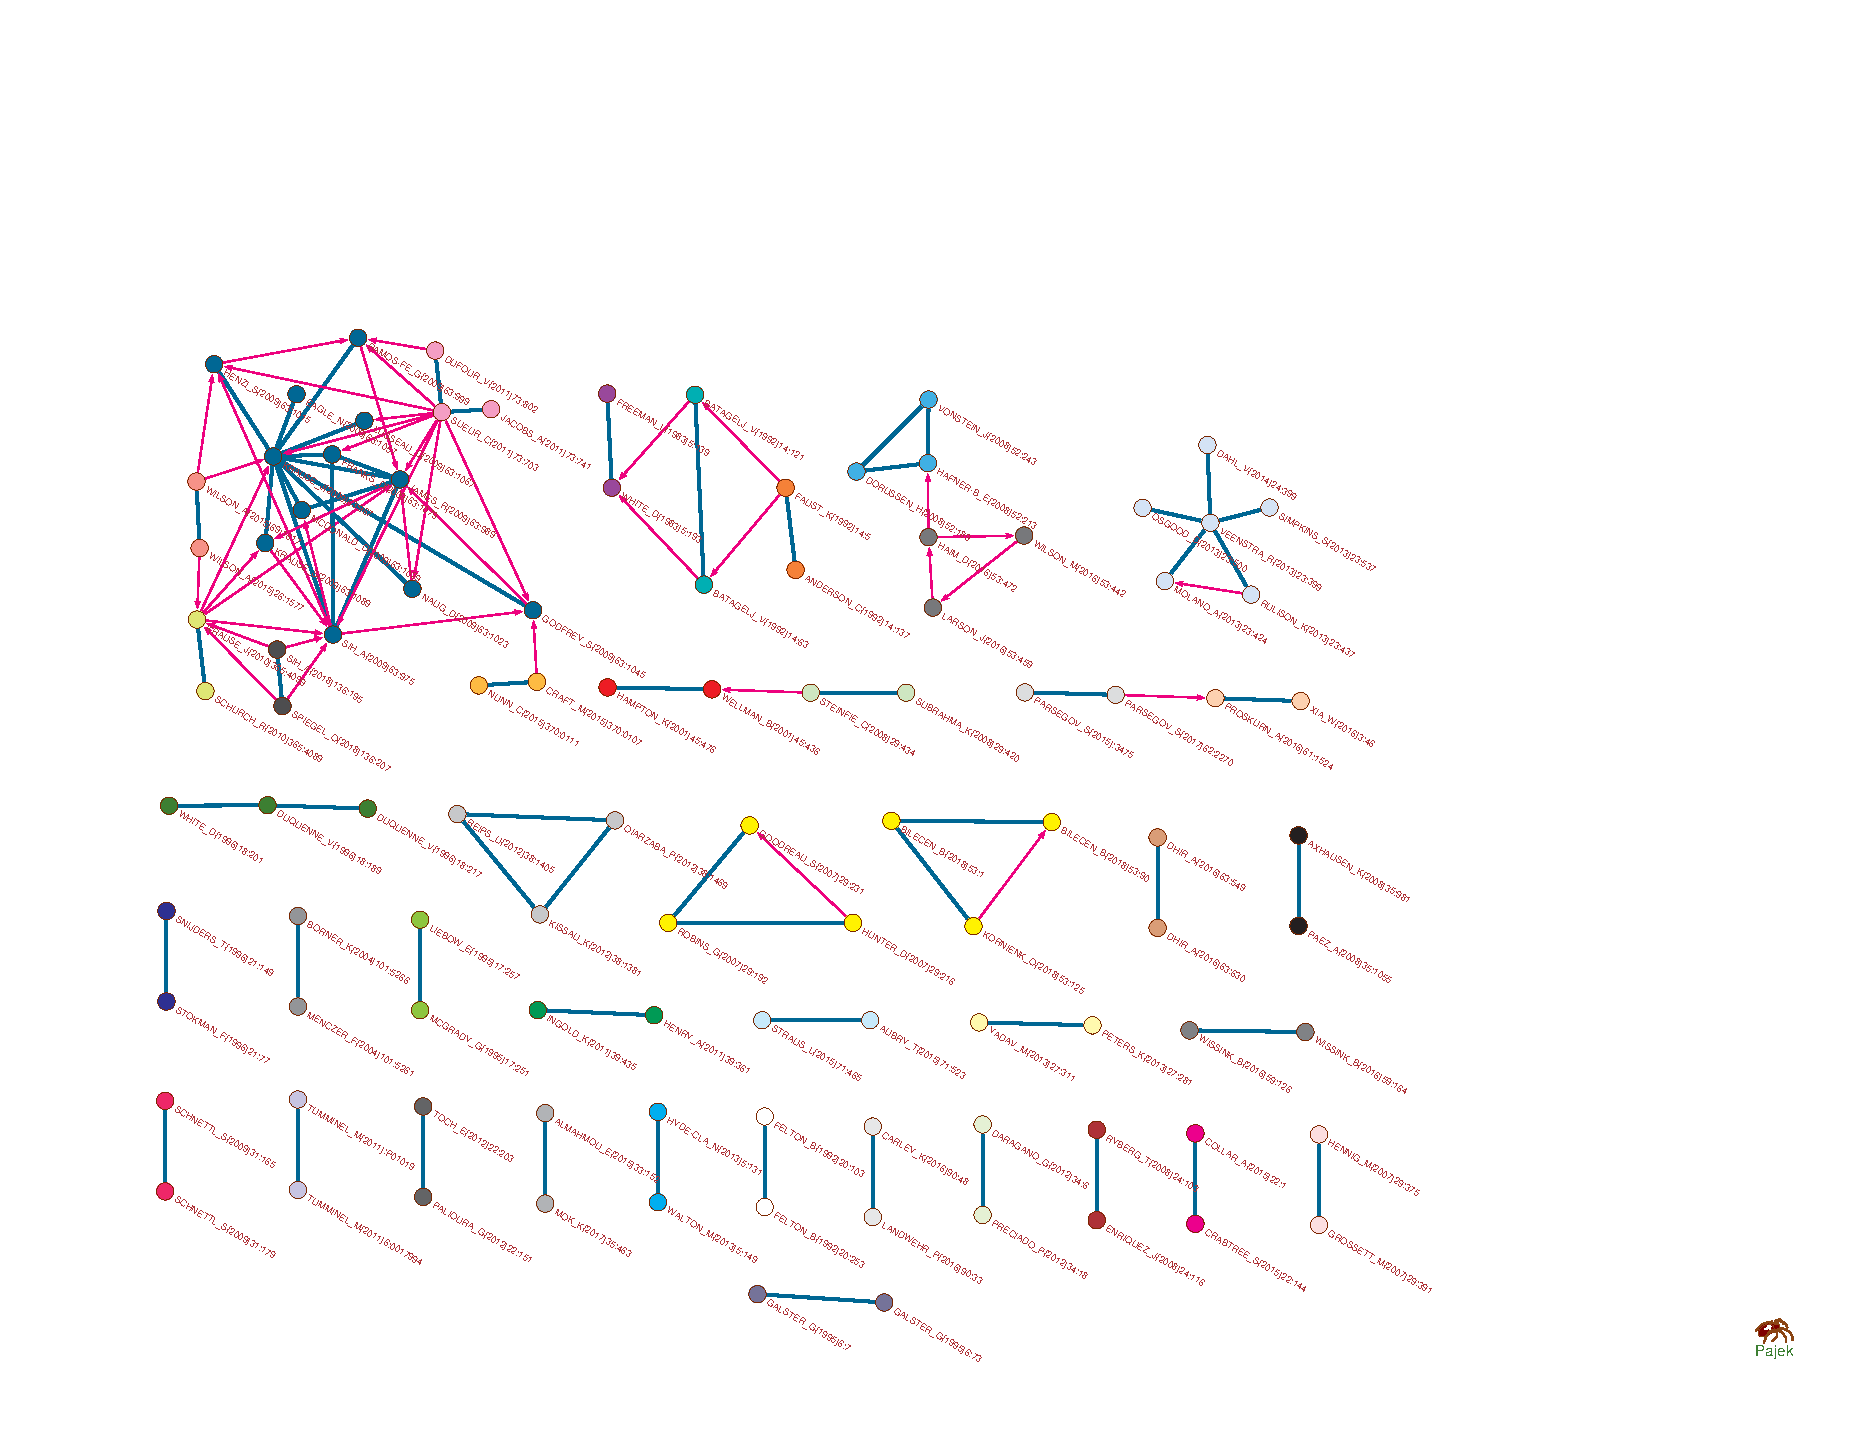
\includegraphics[width=80mm,viewport=75 34 690 535,clip=]{strong.pdf}
\end{center}

\end{frame}

\begin{frame}[fragile]
\frametitle{Main path, Key Routes, and Island 4 \\ \normalsize from SPC network}

\includegraphics[width=10mm,viewport=120 27 235 682 ,clip=]{CPMpath.pdf}
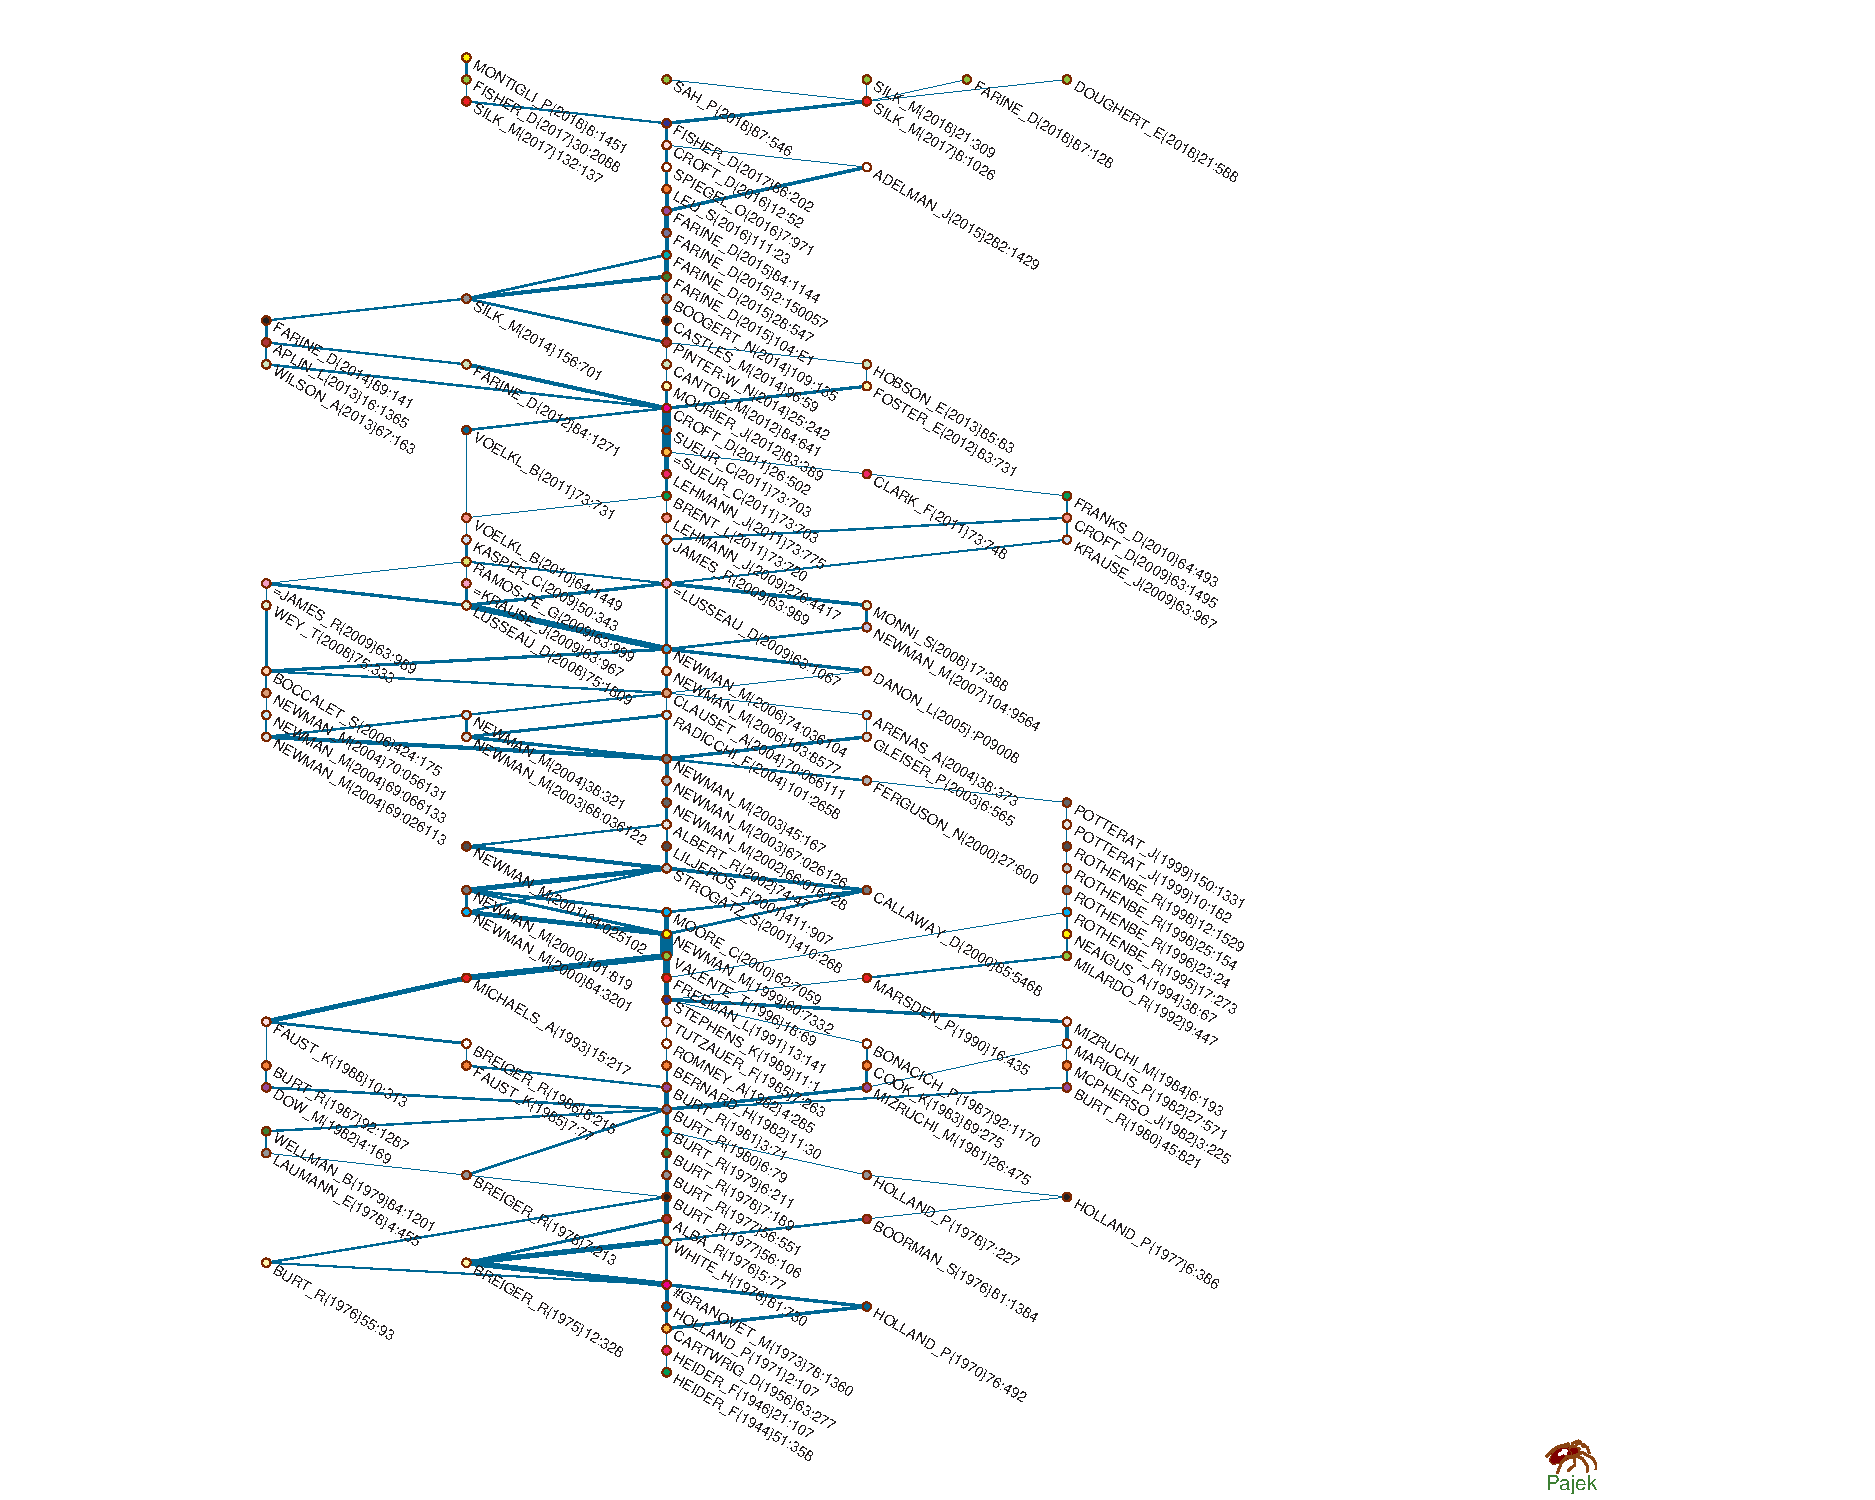
\includegraphics[width=40mm,viewport=120 15 605 700,clip=]{KeyRouteWxy.pdf}
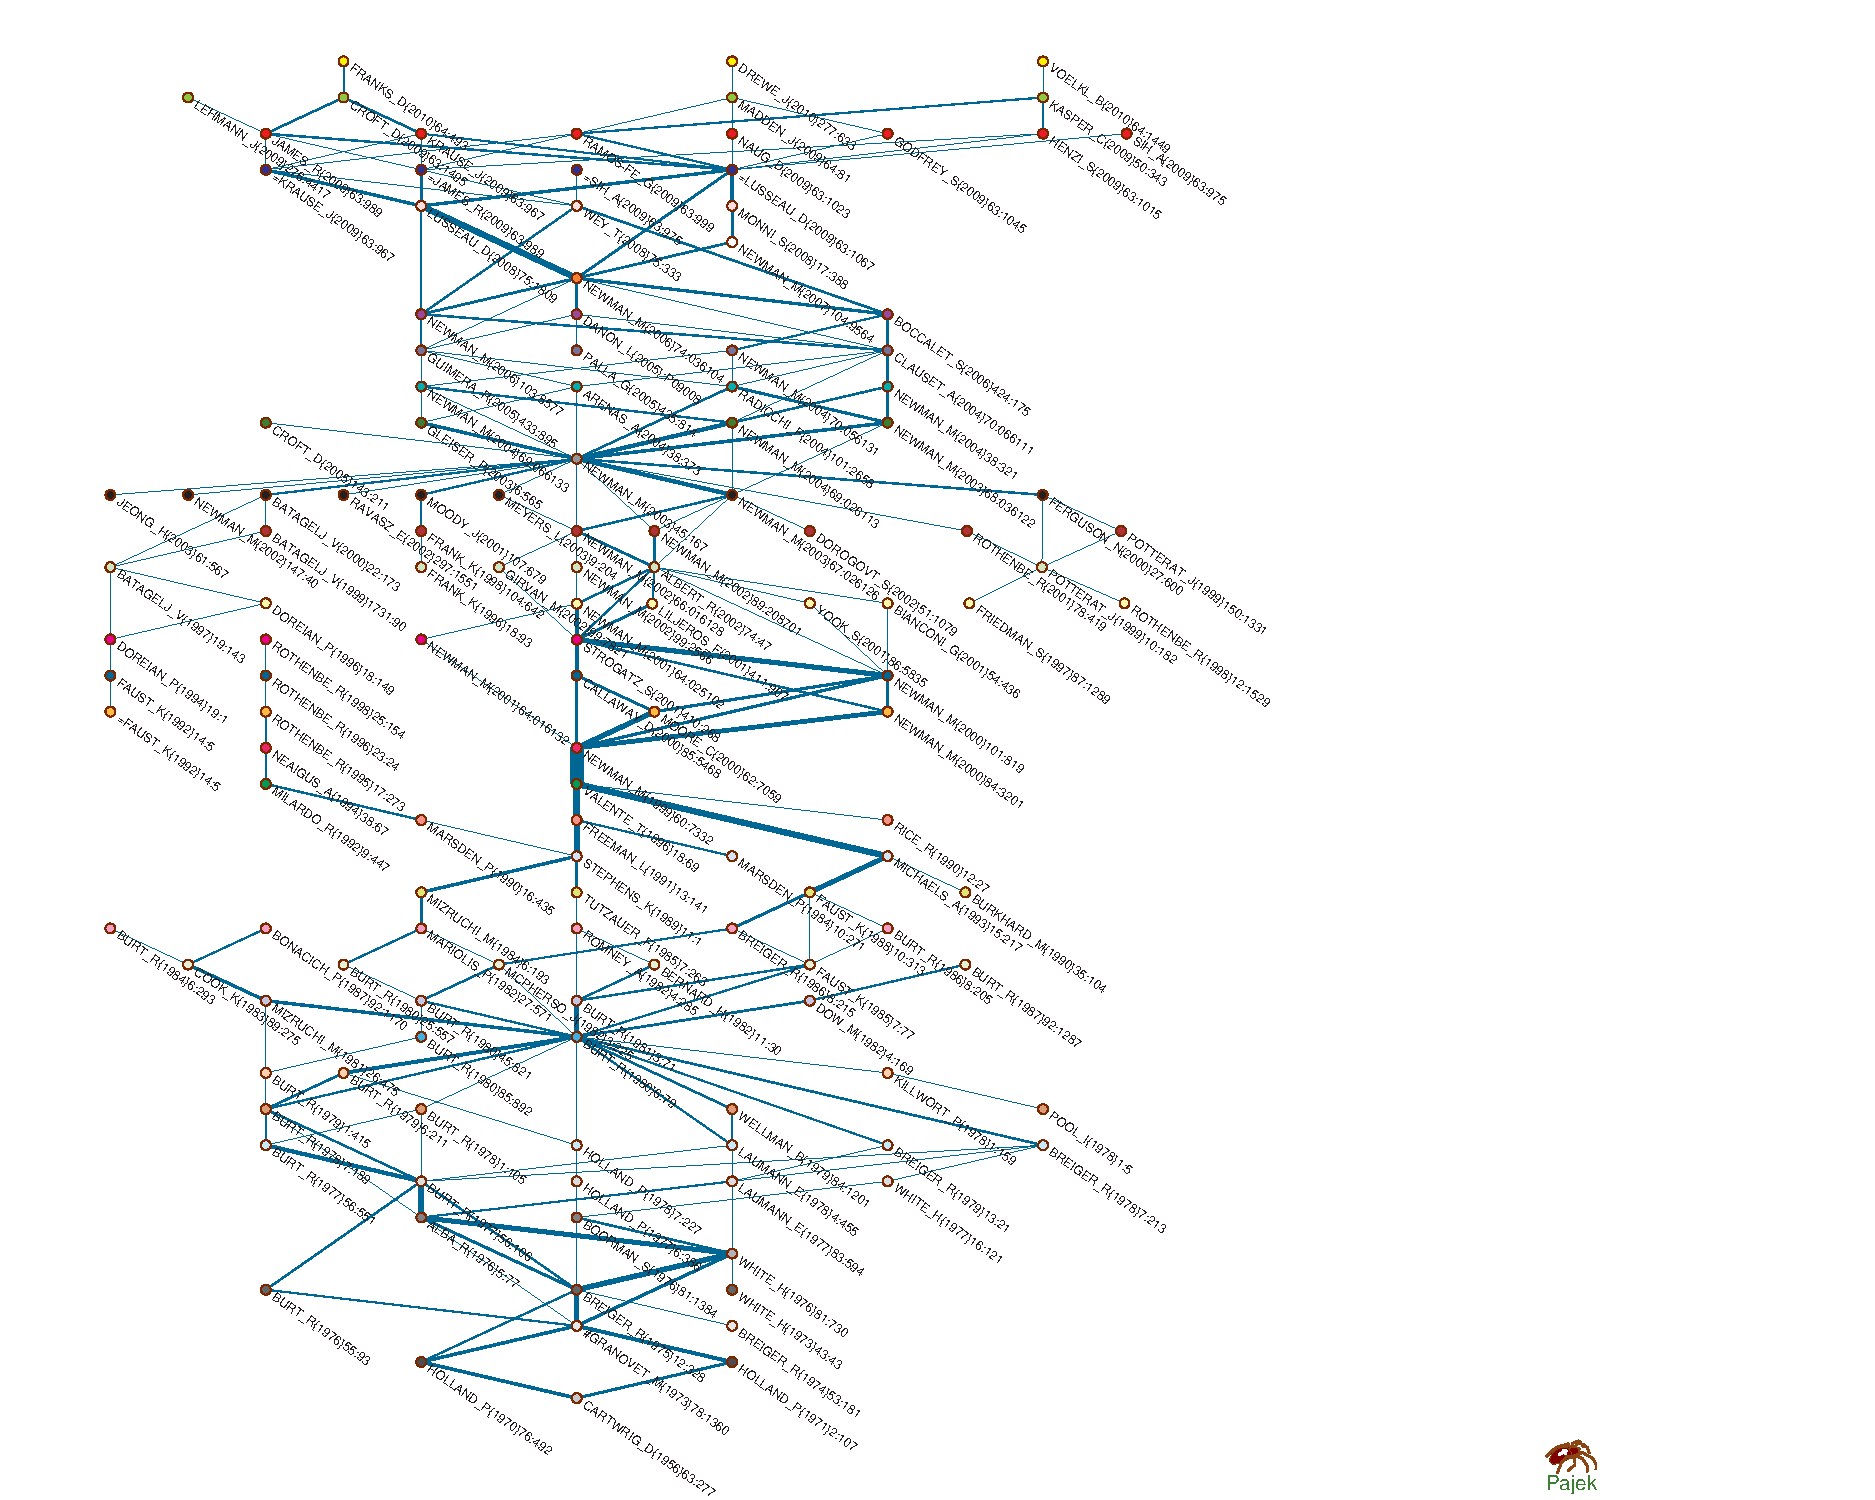
\includegraphics[width=48mm,viewport=45 0 615 695,clip=]{Island4Wxy.pdf}

\end{frame}

\begin{frame}[fragile]
\frametitle{Main path \\ \normalsize from SPC network}

\footnotesize
\begin{enumerate}
\item 1944--1996: 20 works from the field of Social Science in journals \textit{Social networks, Administrative Science Quarterly, Annual Review of Sociology, American Sociological Review, Social Forces, Sociological Methods \& Research, Journal of Mathematical Psychology, Psychological Review, The Journal of Psychology}
\item 1999-2007: 14 works from Physics in journals \textit{Physical Review E, Journal of Statistical Physics, Reviews of Modern Physics, European Physical Journal B, Physics Reports, Nature}, and \textit{SIAM Review}
\item 2008-2018: 25 works from Animal social networks in journals \textit{Animal Behaviour, American Journal of Primatology, Primates, Journal of Evolutionary Biology, Journal of Animal Ecology, Journal of Evolutionary Biology, Trends in Ecology \& Evolution}
\end{enumerate}
\end{frame}

\begin{frame}[fragile]
\frametitle{Key-routes \\ \normalsize from SPC network}

\footnotesize
\textbf{Third period (2008--2018)}: 49 works of  behavioural ecologists. 
\begin{enumerate}
\item Krause, James (2009): \textit{general works} on animal social network analysis
\item Ramos-Fernandez, Kasper, Voell, Lehmann, Brent, Sueur (2009--2011): \textit{social networks of Nonhuman Primates} (monkeys, baboons). 
\item Croft (2011): practical guide on \textit{hypothesis testing} in animal social networks
\item 2014: research on \textit{mixed-species groups} (Farine), \textit{killer whales} (Foster), \textit{sharks} (Mourier), \textit{dolphins} (Cantor), published in 2012, and \textit{birds} (Silk) and \textit{starlings} (Boogert)
\item 2013-2014: \textit{methodological issues} -- Hobson (\textit{An analytical framework for quantifying and testing patterns of temporal dynamics in social networks}), Castels (\textit{Social networks created with different techniques are not comparable}), Pinter-Wollman (\textit{The dynamics of animal social networks: analytical, conceptual, and theoretical advances})
\end{enumerate}
\end{frame}

\begin{frame}[fragile]
\frametitle{Key-routes \\ \normalsize from SPC network}
\footnotesize
\begin{enumerate}
\item Farine (2015): \textit{methodological issues on constructing, conducting and interpreting animal social network analysis}, study of the \textit{wild birds territory acquisition}.
\item 2013-2014: \textit{social personality and phenotypic types} (Wilson, Alpin, Farine). 
\item 2016--2018: studies on \textit{desease transmission} (Adelman, Sah, Silk, Dougherty), \textit{animal paths tracking} (Leu, Spiegel); works on \textit{theoretical issues} (\textit{Current directions in animal social networks} by Croft, \textit{Social traits, social networks and evolutionary biology} by Fisher); \textit{implementation of different models of network analysis to animal behaviour research}:  exponential random graph models and statistical network models (Silk), the potential of stochastic actor-oriented models (Fisher),  dynamic vs. static social network analysis (Farine). \medskip   
\end{enumerate}
\end{frame}

\begin{frame}[fragile]
\frametitle{Islands 1-3, 5 \\ \normalsize from SPC network}
\tiny 
1 - Education, 2 - Physics, 3 - Neuropsychiatry, 5 - Animal SNA
\begin{center}
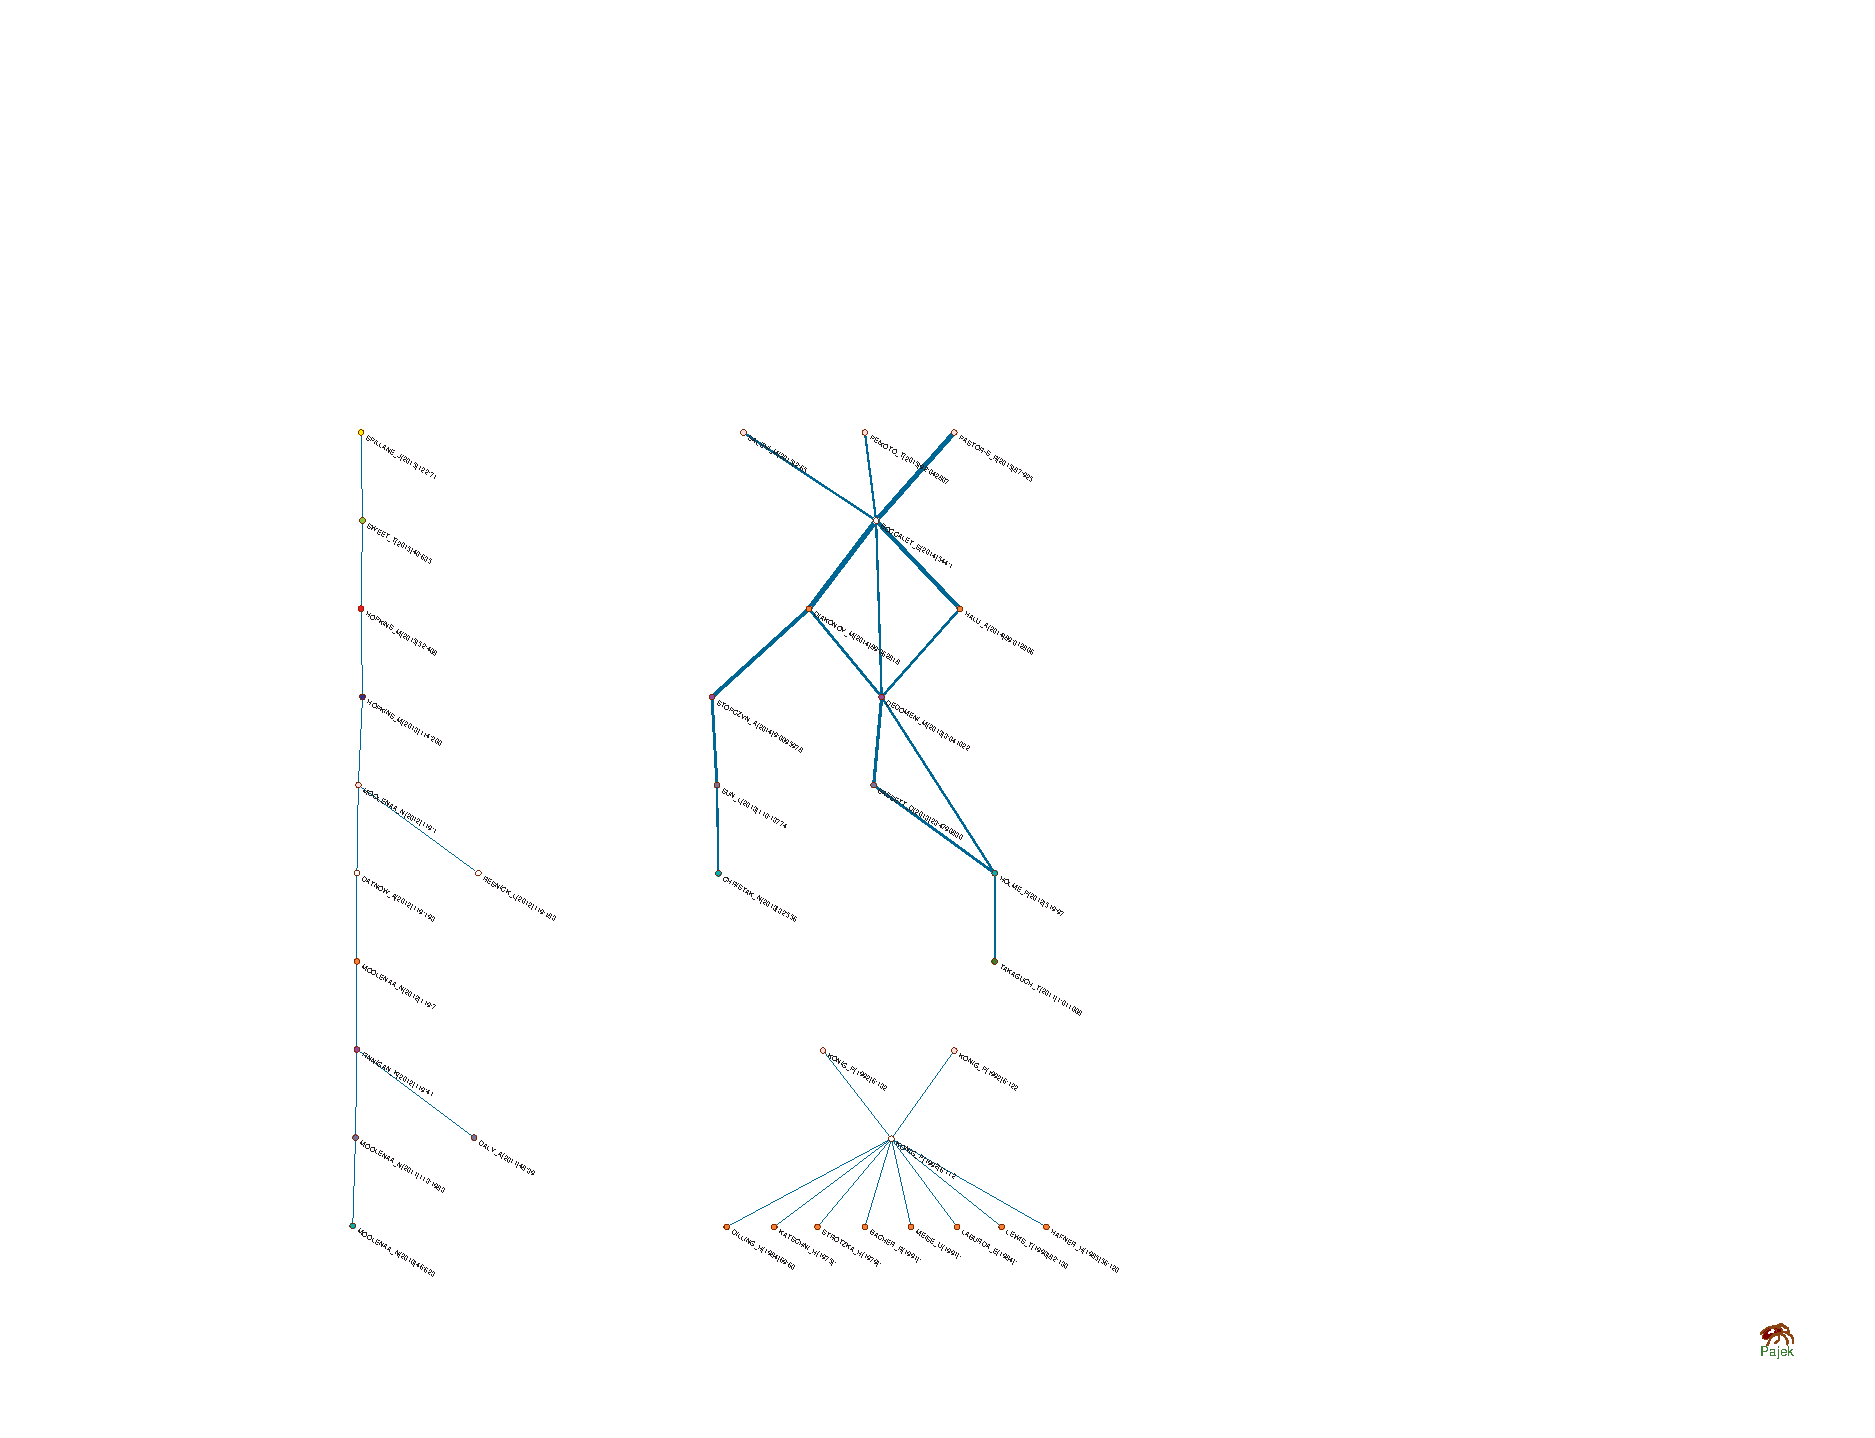
\includegraphics[width=60mm,viewport=160 75 540 488 ,clip=]{Island1-3w.pdf}
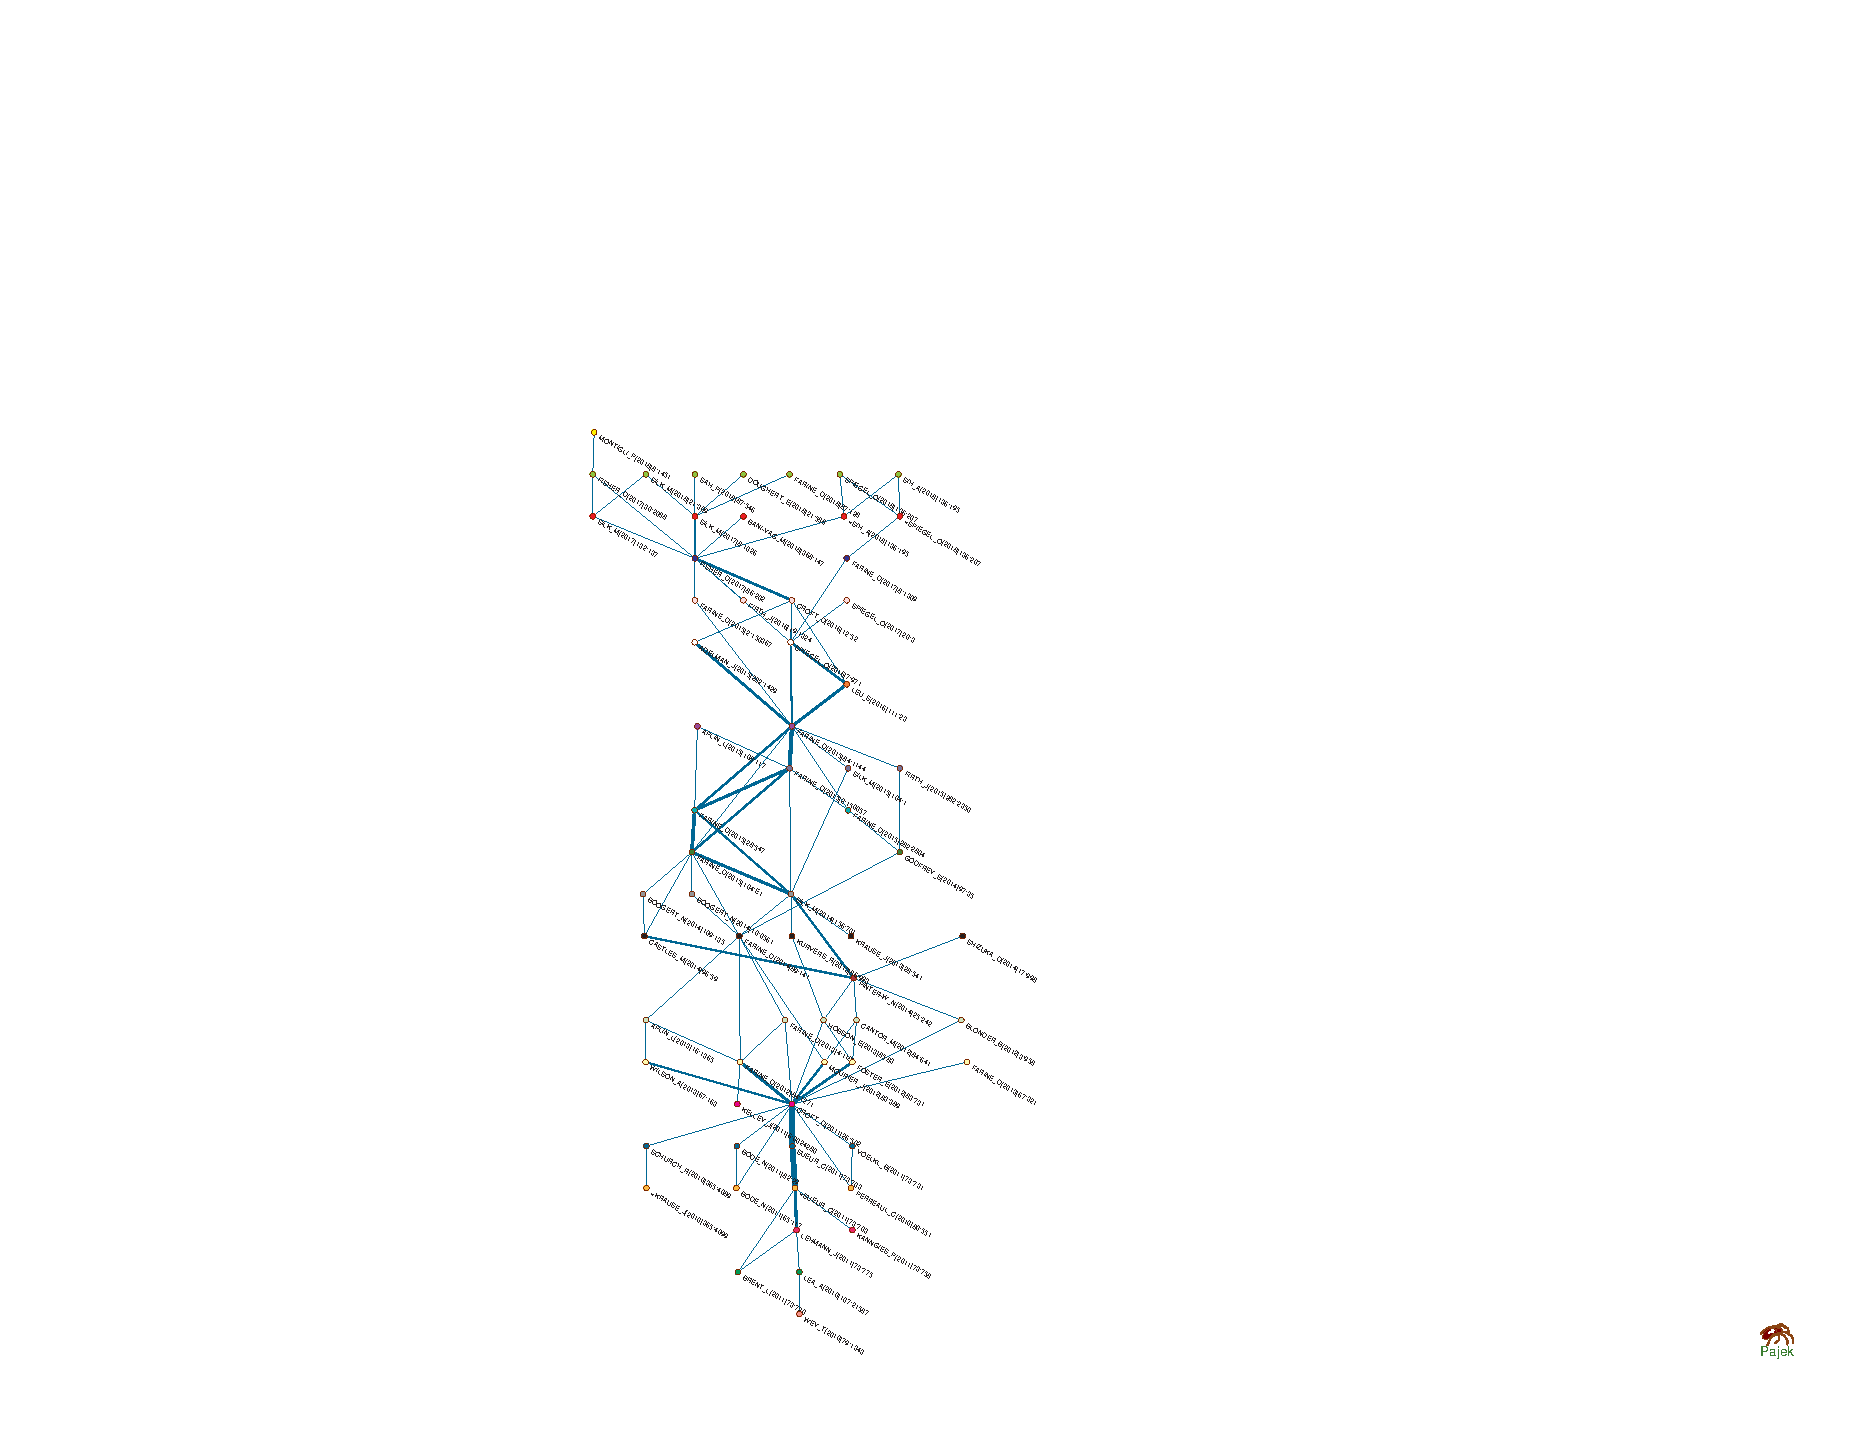
\includegraphics[width=33mm,viewport=280 37 500 488,clip=]{Island5w.pdf}
\end{center}

\end{frame}


\begin{frame}[fragile]
\frametitle{Most important works \\ \normalsize from Probabilistic  Flow network}
\small

\renewcommand{\arraystretch}{0.82}
\tiny
The values were maximized by 1,000,000. 
\begin{tabular}{c|c|l||c|c|l|l}
Rank&   	Value&   	Id&   	Rank&   	Value&   	Id\\ \hline
1&   	4691&   	WASSERMA\_S(1994):&   	31&   	545&   	BLONDEL\_V(2008):P10008\\
2&   	2941&   	WATTS\_D(1998)393:440&   	32&   	527&   	KATZ\_L(1953)18:39\\
3&   	2676&   	GRANOVET\_M(1973)78:1360&   	33&   	526&   	NEWMAN\_M(2010):\\
4&   	2445&   	BOYD\_D(2007)13:210&   	34&   	520&   	STROGATZ\_S(2001)410:268\\
5&   	2241&   	BARABASI\_A(1999)286:509&   	35&   	517&   	PALLA\_G(2005)435:814\\
6&   	1926&   	FREEMAN\_L(1979)1:215&   	36&   	499&   	CLAUSET\_A(2004)70:066111\\
7&   	1396&   	GIRVAN\_M(2002)99:7821&   	37&   	497&   	ERDOS\_P(1960)5:17\\
8&   	1299&   	NEWMAN\_M(2003)45:167&   	38&   	488&   	ROGERS\_E(2003):\\
9&   	1227&   	MCPHERSO\_M(2001)27:415&   	39&   	485&   	NEWMAN\_M(2006)103:8577\\
10&   	1158&   	ALBERT\_R(2002)74:47&   	40&   	481&   	COLEMAN\_J(1990):\\
11&   	1105&   	SCOTT\_J(2000):&   	41&   	478&   	BRIN\_S(1998)30:107\\
12&   	1098&   	BURT\_R(1992):&   	42&   	477&   	AMARAL\_L(2000)97:11149\\
13&   	1045&   	MILGRAM\_S(1967)1:61&   	43&   	475&   	ERDOS\_P(1959)6:290\\
14&   	1013&   	NEWMAN\_M(2004)69:026113&   	44&   	465&   	WATTS\_D(1999):\\
15&   	928&   	KAPLAN\_A(2010)53:59&   	45&   	462&   	LAVE\_J(1991):\\
16&   	878&   	FREEMAN\_L(1977)40:35&   	46&   	460&   	KLEINBER\_J(1999)46:604\\
17&   	852&   	PUTNAM\_R(2000):&   	47&   	449&   	SCOTT\_J(1991):\\
18&   	847&   	COLEMAN\_J(1988)94:95&   	48&   	446&   	BOLLOBAS\_B(1985):\\
19&   	835&   	* BLEI\_D(2003)3:993&   	49&   	442&   	PAGE\_L(1999):\\
20&   	742&   	GRANOVET\_M(1985)91:481&   	50&   	440&   	NEWMAN\_M(2001)64:025102\\
21&   	731&   	CHRISTAK\_N(2007)357:370&   	51&   	436&   	NEWMAN\_M(2004)69:066133\\
22&   	727&   	EVERETT\_M(2002):&   	52&   	431&   	REDNER\_S(1998)4:131\\
23&   	726&   	NEWMAN\_M(2001)98:404&   	53&   	429&   	CHRISTAK\_N(2008)358:2249\\
24&   	719&   	* ALBERT\_R(1999)401:130&   	54&   	424&   	ADOMAVIC\_G(2005)17:734\\
25&   	701&   	* O'REILLY\_T(2005):&   	55&   	424&   	KEMP\_D(2003):137\\
26&   	669&   	BORGATTI\_S(2002):&   	56&   	423&   	DOMINGOS\_P(2001):57\\
27&   	667&   	FORTUNAT\_S(2010)486:75&   	57&   	423&   	MITCHELL\_J(1969):\\
28&   	633&   	HANNEMAN\_R(2005):&   	58&   	415&   	ALBERT\_R(2000)406:378\\
29&   	569&   	STEINFIE\_C(2007)12:1143&   	59&   	415&   	GLASER\_B(1967):\\
30&   	549&   	ZACHARY\_W(1977)33:452&   	60&   	410&   	ROGERS\_E(1995):\\ \hline
\end{tabular}

\end{frame}

\begin{frame}[fragile]
\frametitle{Cite net\\ \normalsize Overlapping of components}
\small

\renewcommand{\arraystretch}{0.2}
\tiny
\begin{tabular}{c|l|l|l|l|}
i&   	name & title & jour & comp \\ \hline 
1&   	Granovet M &   	 Strength of weak ties&   	amer j sociol&   	1, 2, 4, 5, 6\\
2&   	Newman M&   	 The structure and function of complex networks&   	siam rev&   	1, 2, 4, 5, 6\\
3&   	Albert R&   	 Statistical mechanics of complex networks&   	rev mod phys&   	1, 2, 4, 5, 6\\
4&   	Boccaletti S&   	 Complex networks: structure and dynamics&   	phys rept&   	1, 2, 4, 5, 6\\
5&   	White H&   	 Soc. str. from mult. nets. Blockmodels &   	amer j sociol&   	1, 2, 4, 5, 6\\
6&   	Newman M&   	 Clustering and pref.l attach. in growing nets&   	phys rev e&   	1, 2, 4, 5, 6\\
7&   	Newman M&   	 Finding and evaluating comm. struct. in nets&   	phys rev e&   	1, 2, 4, 5, 6\\
8&   	Newman M&   	 Mixing patterns in networks&   	phys rev e&   	1, 2, 4, 5, 6\\
9&   	Strogatz S&   	 Exploring complex networks&   	nature&   	1, 2, 4, 5, 6\\
10&   	Newman M&   	 Detecting community structure in nets&   	eur phys j b&   	1, 2, 4, 5, 6\\
11&   	Newman M&   	 Spread of epidemic disease on nets&   	phys rev e&   	1, 2, 4, 5, 6\\
12&   	Newman M&   	 Finding community str. in nets using eigenvectors &   	phys rev e&   	1, 2, 4, 5, 6\\
13&   	Cartwright D&   	 Structural balance - a generaliz. of heider theory&   	psychol rev&   	1, 2, 4, 5, 6\\
14&   	Clauset A&   	 Finding community struct. in very large nets&   	phys rev e&   	1, 2, 4, 5, 6\\
15&   	Newman M&   	 Models of the small world&   	j statist phys&   	1, 2, 4, 5\\
16&   	Newman M&   	 Scaling and percolation in small-world net model&   	phys rev e&   	1, 2, 4, 5\\
17&   	Valente T&   	 Social net thresholds in the diff. of innov.&   	soc networks&   	1, 2, 4, 5\\
18&   	Burt R&   	 Cohesion versus structural equivalences&   	soc meth res&   	1, 2, 4, 5\\
&   	&   	as a basis for net subgroups&   	&   	\\
19&   	Stephenson K&   	 Rethinking centrality - methods and examples&   	soc networks&   	1, 2, 4, 5\\
20&   	Breiger R&   	 Algorithm for clustering relational data  &   j math psychl&   	1, 2, 4, 5\\
21&   	Freeman L&   	 Centrality in valued graphs - a measure &   soc networks&   	1, 2, 4, 5\\
&   	&   	 of betweenness based on net flow&   	&   	\\
22&   	Burt R&   	 Models of network structure&   	annu rev soc&   	1, 2, 4, 5\\
23&   	Holland P&   	 Method for detecting structure in sociom. data&   amer j sociol&   	1, 2, 4, 5\\
24&   	Alba R&   	 Intersection of social circles &   socl meth res&   	1, 2, 4, 5\\
25&   	Moore C&   	 Exact solution of site and bond percolation &   	phys rev e&   	1, 2, 4, 5\\
&   	&   	on small-world net&   	&   	\\
26&   	Mcpherson J&   	 Hypernetwork sampling - duality and &   	soc networks&   	1, 2, 4, 5\\
&   	&   	 differentiation among voluntary organizations&   	&   \\
27&   	Mariolis P&   	 Centrality in corporate interlock networks &   	adm sci quart&   	1, 2, 4, 5\\
28&   	Burt R&   	 Positions in multiple network systems &   	soc forces&   	1, 2, 4, 5\\
&   	&   	1. General conception of stratification and prestige &   	&   \\
29&   	Burt R&   	 Positions in multiple network systems &   	soc forces&   	1, 2, 4, 5\\
&   	&   	2. Stratification and prestige among elite &   	&   	\\
30&   	Mizruchi M&   Interlock groups, cliques, or interest-groups &   	soc networks&   	1, 2, 4, 5\\ \hline 
\end{tabular}
1- Key Routes, 2- Main Path (CPM), 3- Island5, 4 - Island 4, Node Island, 5 - Prob Flow Island

\end{frame}

%******************************************************************************
\subsection{Collaboration}  

\begin{frame}[fragile]
\frametitle{Authors Collaboration\\ \normalsize Network Co}
\footnotesize

\[ \mathbf{Co} = \mathbf{WAr}^T * \mathbf{WAr} \] 

The weight of the edges between the nodes $i$ and $j$ is equal to total number of works author i and j wrote together. \smallskip 

The loops in $Co$ are equal to the total number of works that each author have (which is also equal to the indegree values of the $WA$ network). \medskip 

The proposed approach has some \keyw{limitations}, such as the overrating of the contribution of works with many authors.

\end{frame}

\begin{frame}[fragile]
\frametitle{Authors Collaboration \\ \normalsize from Co net (20 and more works written together)}

\begin{center}
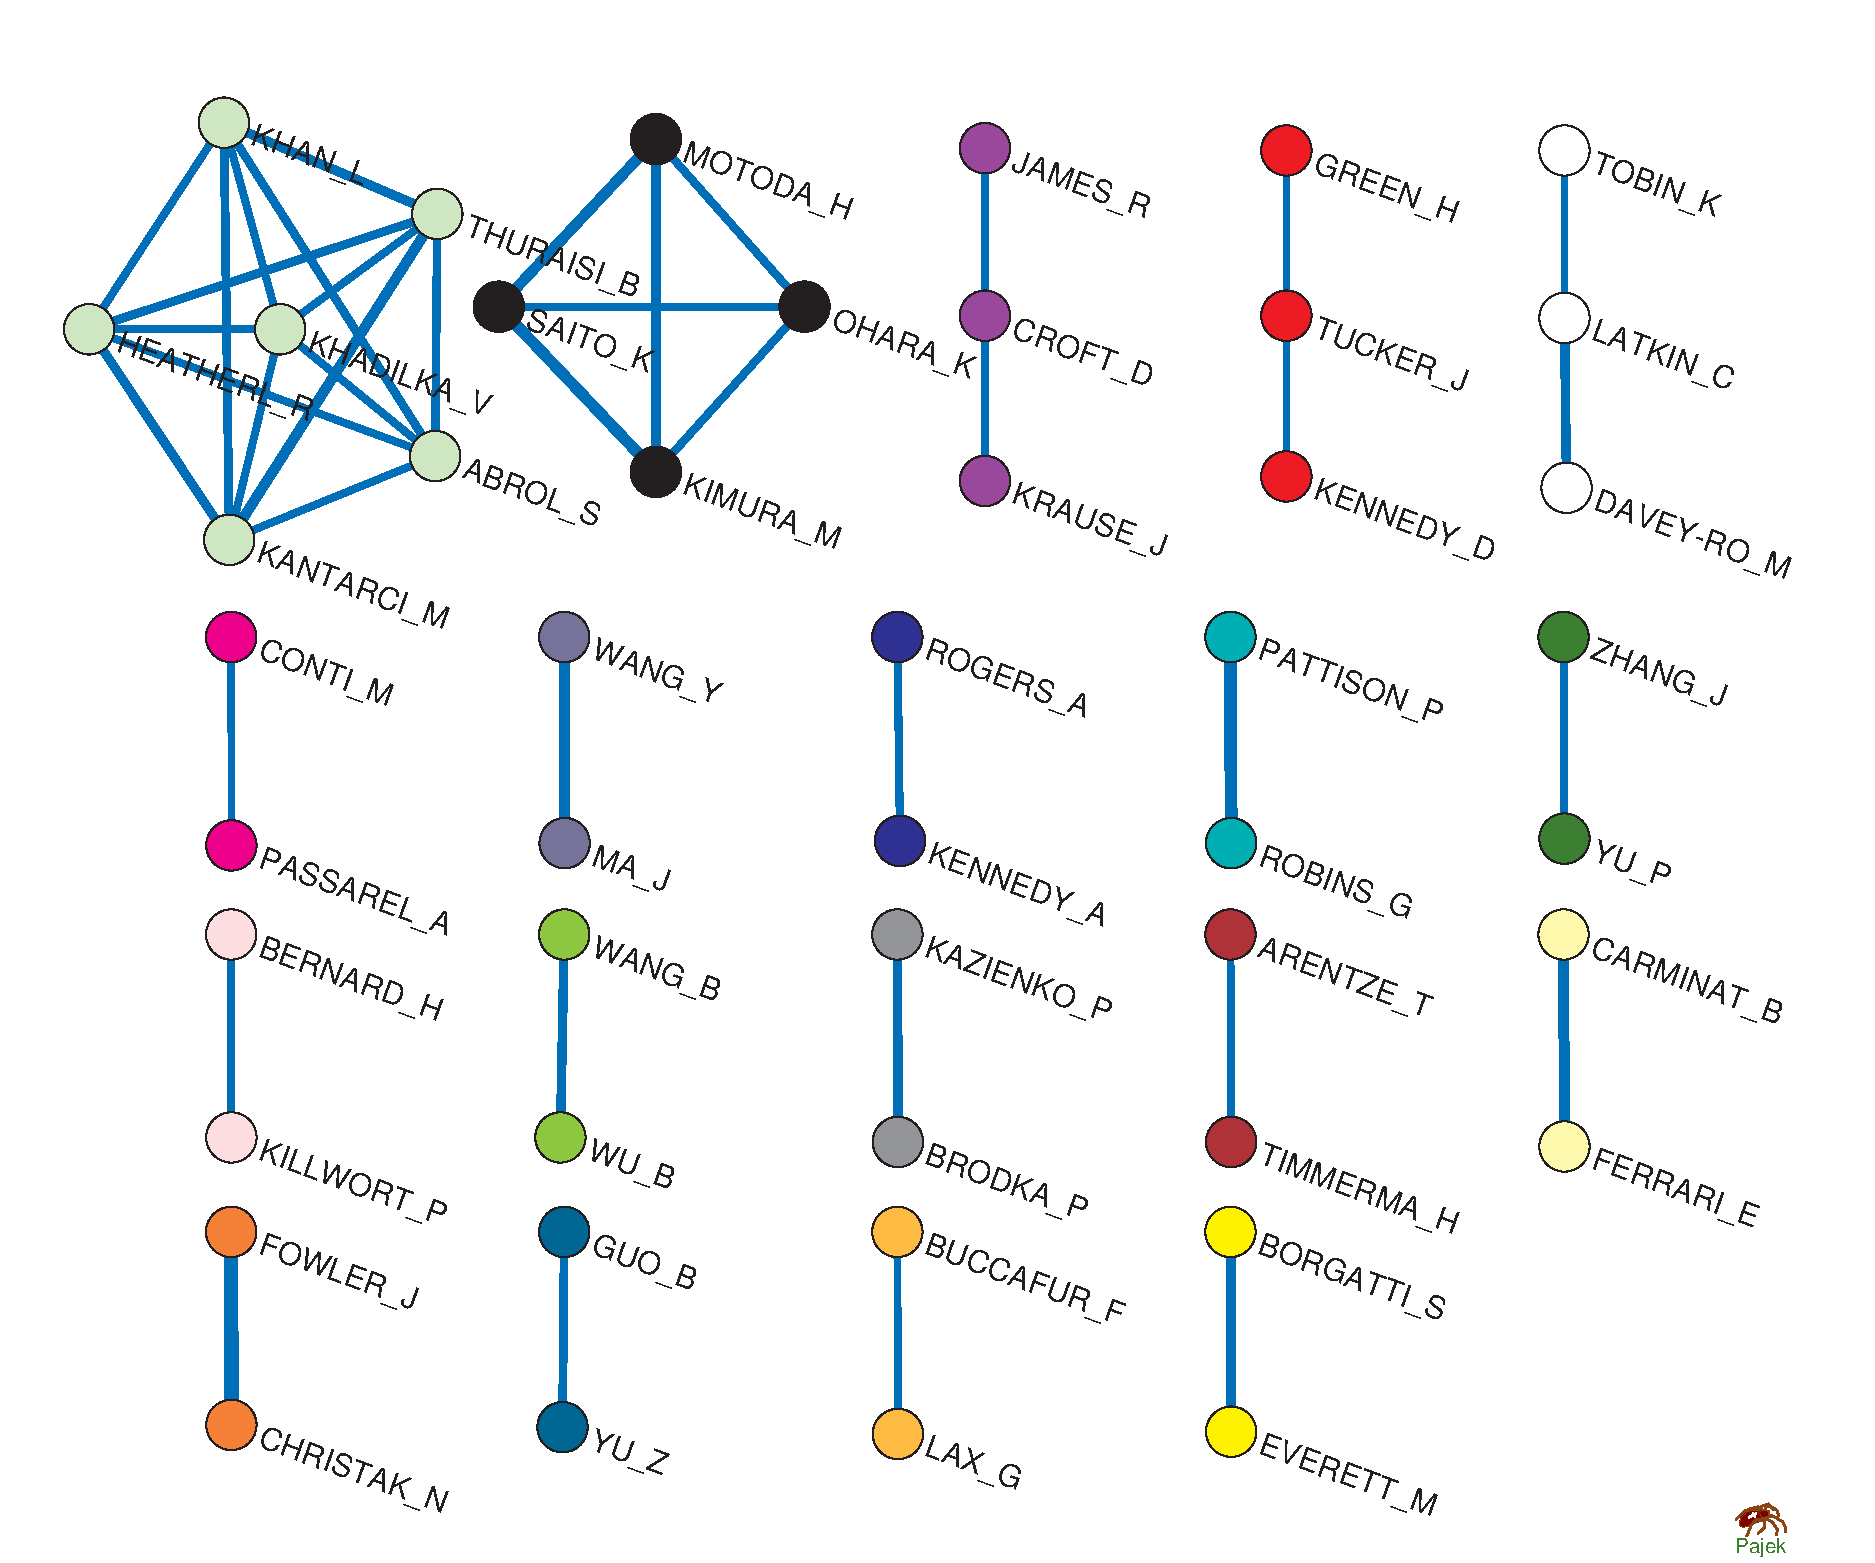
\includegraphics[width=0.7\textwidth]{CoN_Pairs.pdf}
\end{center}

\end{frame}

\begin{frame}[fragile]
\frametitle{Authors Collaboration\\ \normalsize Network Cn}
\footnotesize

The contribution of authors to their own works and works written with co-authors is considered. The normalization create network $n(WA)$ where the weight of each arc is divided by the sum of weights of all arcs having the same initial node as this arc (outdegree of a node).

\[ n(\mathbf{WAr})[w,a] = \frac {\mathbf{WAr}[w,a]}{\max(1,\textrm{Oudeg}[w])}\]
then 
\[ \mathbf{Cn} = \mathbf{WAr}^T * n(\mathbf{WAr}) \] 
 
The weight of the edges between the nodes (authors) is equal to the contribution of author i to works, that he or she wrote together with author j (can be not symmetric). 

The total contribution for an author is equal to the number of works that he or she co-authored (indegree of WA). 

The diagonal (loops) of the matrix is equal to the total contribution of author to his or her own works.

\end{frame}

\begin{frame}[fragile]
\frametitle{Authors Collaboration\\ \normalsize Network Cn}
\footnotesize

Batagelj and Cerinšek (2013):
\begin{itemize}
\item \textbf{self-sufficiency index} as a proportion of author's contribution to all his/her works and her/his total number of works (which is equal to the value of Indegree of $WA$ network), 
\item \textbf{collaborativness index}, which is complementary to it (is equal to 1 minus self-sufficiency).
\end{itemize}
\end{frame}

\begin{frame}[fragile]
\frametitle{Authors Collaboration \\ \normalsize Collaborativeness index from Cn net}

\renewcommand{\arraystretch}{0.82}
\tiny
\begin{tabular}{c|l|p{0.4cm}|p{0.6cm}|p{0.4cm}||c|l|p{0.4cm}|p{0.6cm}|p{0.4cm}|} 
\# & Author & Tot Contr & Tot \#works & Collab & \# & Author & Tot Contr & Tot \#works & Collab \\ \hline
1& 	BURT\_R& 	55,73& 	71& 	0,22& 	31& 	\textbf{PATTISON\_P}& 	18,94& 	58& 	0,67\\
2& 	NEWMAN\_M& 	50,02& 	*81& 	0,38& 	32& 	\textbf{THELWALL\_M}& 	18,41& 	37& 	0,50\\
3& 	DOREIAN\_P& 	46,19& 	72& 	0,36& 	33& 	\textbf{KRACKHAR\_D}& 	18,24& 	38& 	0,52\\
4& 	\textbf{PARK\_H}& 	41,94& 	*113& 	0,63& 	34& 	\textbf{FALOUTSO\_C}& 	17,86& 	60& 	0,70\\
5& 	\textbf{DUNBAR\_R}& 	40,02& 	*91& 	0,56& 	35& 	\textbf{JACKSON\_M}& 	17,78& 	38& 	0,53\\
6& 	WELLMAN\_B& 	36,43& 	63& 	0,42& 	36& 	\textbf{GONZALEZ\_M}& 	17,76& 	52& 	0,66\\
7& 	\textbf{VALENTE}\_T& 	34,96& 	*97& 	0,64& 	37& 	\textbf{MOODY\_J}& 	17,7& 	40& 	0,56\\
8& 	\textbf{PARK\_S}& 	34,59& 	*109& 	0,68& 	38& 	SCOTT\_J& 	17,54& 	28& 	0,37\\
9& 	BONACICH\_P& 	34& 	46& 	0,26& 	39& 	\textbf{MORRIS\_M}& 	17,22& 	43& 	0,60\\
10& 	LEYDESDO\_L& 	33,28& 	51& 	0,35& 	40& 	\textbf{RODRIGUE\_J}& 	15,9& 	52& 	0,69\\
11& 	\textbf{LATKIN\_C}& 	32,99& 	*130& 	0,75& 	41& 	\textbf{WASSERMA\_S}& 	15,64& 	35& 	0,55\\
12& 	LITWIN\_H& 	32,42& 	50& 	0,35& 	42& 	\textbf{KLEINBER\_J}& 	15,05& 	34& 	0,56\\
13& 	MARSDEN\_P& 	30,17& 	39& 	0,23& 	43& 	\textbf{BATAGELJ\_V}& 	14,64& 	33& 	0,56\\
14& 	\textbf{BORGATTI\_S}& 	29,72& 	71& 	0,58& 	44& 	\textbf{WILLIAMS\_A}& 	14,5& 	31& 	0,53\\
15& 	\textbf{SNIJDERS\_T}& 	29,63& 	67& 	0,56& 	45& 	\textbf{SINGH\_A}& 	14,5& 	36& 	0,60\\
16& 	FRIEDKIN\_N& 	28,17& 	36& 	0,22& 	46& 	\textbf{BRANDES\_U}& 	14,39& 	35& 	0,59\\
17& 	\textbf{CARLEY\_K}& 	28,11& 	72& 	0,61& 	47& 	\textbf{BERKMAN\_L}& 	14,3& 	39& 	0,63\\
18& 	\textbf{BARABASI\_A}& 	27,61& 	67& 	0,59& 	48& 	MASUDA\_N& 	14,26& 	28& 	0,49\\
19& 	WHITE\_H& 	27,28& 	42& 	0,35& 	49& 	\textbf{SMITH\_A}& 	14,2& 	40& 	0,65\\
20& 	\textbf{CHRISTAK\_N}& 	22,89& 	74& 	0,69& 	50& 	LAZEGA\_E& 	14,17& 	26& 	0,46\\
21& 	EVERETT\_M& 	22,58& 	44& 	0,49& 	51& 	\textbf{CONTRACT\_N}& 	14,15& 	43& 	0,67\\
22& 	\textbf{KAZIENKO\_P}& 	21,97& 	64& 	0,66& 	52& 	\textbf{GONZALEZ\_A}& 	14,13& 	35& 	0,60\\
23& 	\textbf{MARTINEZ\_M}& 	21,9& 	53& 	0,59& 	53& 	\textbf{PENTLAND\_A}& 	14,12& 	41& 	0,66\\
24& 	\textbf{JOHNSON\_J}& 	21,19& 	54& 	0,61& 	54& 	\textbf{FARINE\_D}& 	14,04& 	34& 	0,59\\
25& 	\textbf{FOWLER\_J}& 	20,14& 	65& 	0,69& 	55& 	\textbf{SCHNEIDE\_J}& 	13,89& 	52& 	0,73\\
26& 	\textbf{SKVORETZ\_J}& 	20,07& 	42& 	0,52& 	56& 	WATTS\_D& 	13,67& 	27& 	0,49\\
27& 	FREEMAN\_L& 	20,03& 	27& 	0,26& 	57& 	FAUST\_K& 	13,5& 	25& 	0,46\\
28& 	BREIGER\_R& 	19,73& 	31& 	0,36& 	58& 	\textbf{SMITH\_M}& 	13,29& 	39& 	0,66\\
29& 	\textbf{ROBINS\_G}& 	19,67& 	64& 	0,69& 	59& 	\textbf{RODRIGUE\_M}& 	13,21& 	46& 	0,71\\
30& 	\textbf{RAHMAN\_M}& 	19,18& 	59& 	0,67& 	60& 	\textbf{RICE\_E}& 	13,09& 	48& 	0,73\\
\end{tabular}

\end{frame}

\begin{frame}[fragile]
\frametitle{Authors Collaboration\\ \normalsize Network Ct'}
\footnotesize

Newman's normalization: “strict collaboration”  -- the weight is a proportion of time spent for the collaboration with each co-author. The weight of each arc is divided by the sum of weights of all arcs having the same initial node as this arc (outdegree of a node) subtracting the initial author.

\[ n'(\mathbf{WAr})[w,a] = \frac{\mathbf{WAr}[w,a]}{\max(1,\textrm{Outdeg}(w)-1)}\]
then 
\[ \mathbf{Ct'} = n(\mathbf{WAr})^T * n'(\mathbf{WAr}) \] 

\medskip

The final $Ct'$ is undirected without loops. The contribution of a complete subgraph corresponding to each work is 1. 

The weights of the edges between the nodes (authors) are equal to the total contribution of “strict collaboration” of authors i and j to works they wrote together.

The total contribution for an author is counted by line weights -- it is equal to the sum of the weights of all the works he or she co-authored. 

\end{frame}


\begin{frame}[fragile]
\frametitle{Authors Collaboration \\ \normalsize Main simple islands from Ct` net}

\begin{center}
\includegraphics[width=80mm,viewport=30 27 830 700,clip=]{Ct`SimIslAll.pdf}
\end{center}


\end{frame}

\begin{frame}[fragile]
\frametitle{Authors Collaboration \\ \normalsize Selected islands from Ct' net}

\begin{center}
\includegraphics[width=0.8\textwidth]{Ct`SimIslSel.pdf}
\end{center}

\end{frame}

\begin{frame}[fragile]
\frametitle{Authors Collaboration \\ \normalsize Authors with largest line weights from Ct' net}

\begin{center}
\includegraphics[width=80mm,viewport=30 22 833 710,clip=]{Ct`largest.pdf}
\end{center}

\end{frame}

\begin{frame}[fragile]
\frametitle{Authors Collaboration \\ \normalsize Selected authors from Ct' net}

\begin{center}
\includegraphics[width=80mm,viewport=40 85 850 660,clip=]{Ct`someAut.pdf}
\end{center}

\end{frame}


\begin{frame}[fragile]
\frametitle{Key words in coauthorship islands \\ \normalsize AK net}

\[ \mathbf{AK} = n(\mathbf{WAr}) ^ T * n(\mathbf{WKr}) \] \medskip

The  weight of the edges between the nodes $a$ and $k$  is equal to the fractional contribution for a given keyword $k$ to the works of author $a$ or a group of authors $C$. 

%AK[C,k] = sum(A[a,k]) : a in C)] 

\[ \mathbf{AK[C,k]} = \sum_{a \in C}\mathbf{AK}[a,k] \] 

\end{frame}


\begin{frame}[fragile]
\frametitle{Key words in coauthorship islands \\ \normalsize AK net }

\scriptsize
\renewcommand{\arraystretch}{0.84}
\begin{center}
\begin{tabular}{p{0.5cm}|p{0.8cm}|p{1.7cm}||p{0.8cm}|p{1.4cm}||p{0.8cm}|p{1.6cm}} \hline \hline
& \multicolumn{2}{c}{BORGATTI\_S}		& \multicolumn{2}{c}{BARABASI\_A}  & \multicolumn{2}{c}{CHRISTAKIS\_K}\\ \hline \hline
      Rank 	&   Value  & Id		    & 	   Value  & Id		       &	 Value  & Id	    \\ \hline
         1 	&  4.9303  & network	    &	    7.0709  & network	       &	  3.1788 &  network	    \\
         2 	&  2.5918  & social	    &	    2.0782  & social	       &	  2.9358 &  social	    \\
         3 	&  2.0858  & graph	    &	    1.7068  & dynamics	       &	  1.0204 &  spread	    \\
         4 	&  1.4210  & centrality	    &	    1.6670  & complex	       &	  1.0192 &  behavior	    \\
         5 	&  1.4202  & analysis	    &	    1.6362  & scale	       &	  0.7261 &  health	    \\
         6 	&  1.3399  & role	    &	    1.5946  & web	       &	  0.5512 &  large	    \\
         7 	&  1.2780  & regular	    &	    1.5516  & community	       &	  0.5169 &  model	    \\
         8 	&  1.2424  & equivalence    &	    1.4709  & world	       &	  0.4778 &  smoking	    \\
         9 	&  1.0530  & semigroup	    &	    1.3622  & internet	       &	  0.4522 &  human	    \\
        10 	&  1.0000  & correction	    &	    1.1906  & model	       &	  0.4479 &  cooperation	    \\
        11 	&  0.9891  & structure	    &	    1.1858  & free	       &	  0.4313 &  obesity	    \\
        12 	&  0.7755  & clique	    &	    1.0210  & evolve	       &	  0.4125 &  influence	    \\
        13 	&  0.7576  & homomorphism   &	    1.0087  & science	       &	  0.3973 &  life	    \\
        14 	&  0.7241  & relation	    &	    0.9808  & random	       &	  0.3728 &  dynamics	    \\
        15 	&  0.6346  & power	    &	    0.9476  & wide	       &	  0.3715 &  evolution	    \\
        16 	&  0.6301  & betweenness    &	    0.8178  & human	       &	  0.3463 &  analysis	    \\
        17 	&  0.6287  & exchange	    &	    0.8076  & theory	       &	  0.3286 &  cosponsorship   \\
        18 	&  0.6232  & algorithm	    &	    0.7561  & small	       &	  0.3044 &  norm	    \\
        19 	&  0.6167  & similarity	    &	    0.7536  & graph	       &	  0.3036 &  trial	    \\
        20 	&  0.5595  & ebloc	    &	    0.6603  & phenomenon       &	  0.2985 &  study	    \\ \hline
     Sum: & 63.0810	& 		  &   76.6373		& 		&  46.8865	  & 		    \\  \hline\hline
\end{tabular}
\end{center}

\end{frame}
    
\begin{frame}[fragile]
\frametitle{Key words in coauthorship islands \\ \normalsize from AK net (nAWr x nWKr)}

\scriptsize
\renewcommand{\arraystretch}{0.84}
\begin{center}
\begin{tabular}{p{0.5cm}|p{0.8cm}|p{1.7cm}||p{0.8cm}|p{1.4cm}||p{0.8cm}|p{1.6cm}} \hline \hline    
 & \multicolumn{2}{c}{PATTISON\_P} &  \multicolumn{2}{c}{SNIJDERS\_T}	  & 	 \multicolumn{2}{c}{VALENTE\_T} \\ \hline\hline
        Rank   &   Value  & Id		    & 	   Value  & Id		       &	 Value  & Id	    \\ \hline
           1   & 	2.2196  &  network	    & 	2.6375  &	 network	    &	    2.5536  &	 network	   \\
           2   & 	2.0729  &  social	    &	2.0902  &	 social		    &	    1.9553  &	 social	   \\
           3   & 	1.7567  &  model	    &	1.6702  &	 model		    &	    1.0000  &	 untitled	   \\
           4   & 	1.3084  &  graph	    &	1.0692  &	 graph		    &	    0.9419  &	 health	   \\
           5   & 	0.8939  &  random	    &	0.8857  &	 dynamics	    &	    0.8737  &	 diffusion	   \\
           6   & 	0.8583  &  markov	    &	0.7390  &	 markov		    &	    0.7802  &	 behavior	   \\
           7   & 	0.8531  &  logit	    &	0.6903  &	 random		    &	    0.7402  &	 innovation	   \\
           8   & 	0.8220  &  logistic	    &	0.6734  &	 friendship	    &	    0.6974  &	 model	   \\
           9   & 	0.8220  &  regression	    &	0.6228  &	 datum		    &	    0.6521  &	 use	   \\
          10   & 	0.8012  &  exponential	    &	0.5932  &	 statistical	    &	    0.6349  &	 peer	   \\
          11   & 	0.7055  &  analysis	    &	0.5780  &	 behavior	    &	    0.6216  &	 adolescent	   \\
          12   & 	0.6752  &  p		    &	0.5547  &	 analysis	    &	    0.5717  &	 influence	   \\
          13   & 	0.5530  &  statistical	    &	0.5423  &	 peer		    &	    0.5610  &	 smoking	   \\
          14   & 	0.5038  &  structure	    &	0.5383  &	 inference	    &	    0.5371  &	 analysis	   \\
          15   & 	0.3561  &  semigroup	    &	0.5346  &	 influence	    &	    0.5247  &	 prevention	   \\
          16   & 	0.3522  &  asterisk	    &	0.4623  &	 stochastic	    &	    0.4987  &	 cigarette	   \\
          17   & 	0.3368  &  process	    &	0.4612  &	 actor		    &	    0.4979  &	 opinion	   \\
          18   & 	0.3333  &  multirelational  &	0.4480  &	 selection	    &	    0.4860  &	 leader	   \\
          19   & 	0.3249  &  family	    &	0.4372  &	 longitudinal	    &	    0.4545  &	 risk	   \\
          20   & 	0.3031  &  dynamics	    &	0.3785  &	 orient		    &	    0.4491  &	 intervention  \\ \hline
       Sum:    & 38.6110	& 		    &	46.6732 &	&       	    44.8812&	 	   \\ \hline
\end{tabular}
\end{center}

\end{frame}

%******************************************************************************
\subsection{Citation} 

\begin{frame}[fragile]
\frametitle{Citation among authors \\ \normalsize CiteA and CiteAn nets}
\footnotesize

\[ \mathbf{CiteA} = (\mathbf{WAr}) ^ T * \mathbf{CiteR} * \mathbf{WAr} \] 

The value of weight of the element [u,v] is equal to the \textbf{absolute number of citations} from works coauthored by $u$ to works coauthored by $v$. \smallskip

\[ \mathbf{CiteAn} = (\mathbf{WAr}) ^ T * n(\mathbf{CiteR}) * \mathbf{WAr} \]  
where 
\[ n(\mathbf{CiteR})[u,v] = \frac {\mathbf{CiteR}[u,v]}{\max(1,\textrm{outdeg}(u))}\]

The value of element CiteAn[u,v] is equal to the number of \textbf{fractional contribution} of citations from works coauthored by $u$ to works coauthored by $v$.\smallskip

\end{frame}

\begin{frame}[fragile]
\frametitle{Citation among authors \\ \normalsize self-citation from CiteA net}

\renewcommand{\arraystretch}{0.95}
\footnotesize
\begin{center}
\begin{tabular}{c|l|l|c|l|l|} 
     Rank  &     Value  & Id		 &    Rank  &     Value  & Id	   \\  \hline  
        1  &  589  & DUNBAR\_R	&    11  &  201  & BARABASI\_A	   \\
        2  &  387  & LATKIN\_C	&    12  &  191  & FARINE\_D	   \\
        3  &  292  & CHRISTAK\_N	&    13  &  188  & SNIJDERS\_T	   \\
        4  &  280  & VALENTE\_T	&    14  &  153  & WELLMAN\_B	   \\
        5  &  268  & BURT\_R	      	&    15  &  148  & DOREIAN\_P	   \\
        6  &  248  & NEWMAN\_M	&    16  &  146  & BORGATTI\_S	   \\
        7  &  232  & ROBINS\_G	&    17  &  146  & ZENOU\_Y	   \\    
        8  &  224  & PATTISON\_P	&    18  &  143  & RICE\_E	   \\    
        9  &  221  & FOWLER\_J	&    19  &  142  & JAMES\_R	   \\    
       10  &  204  & CROFT\_D	      	&   20   & 141   & KRAUSE\_J	    \\ \hline 
\end{tabular} 
\end{center}

\end{frame}

\begin{frame}[fragile]
\frametitle{Citation among authors \\ \normalsize Authors with largest line weights from CiteA net}

\begin{center}
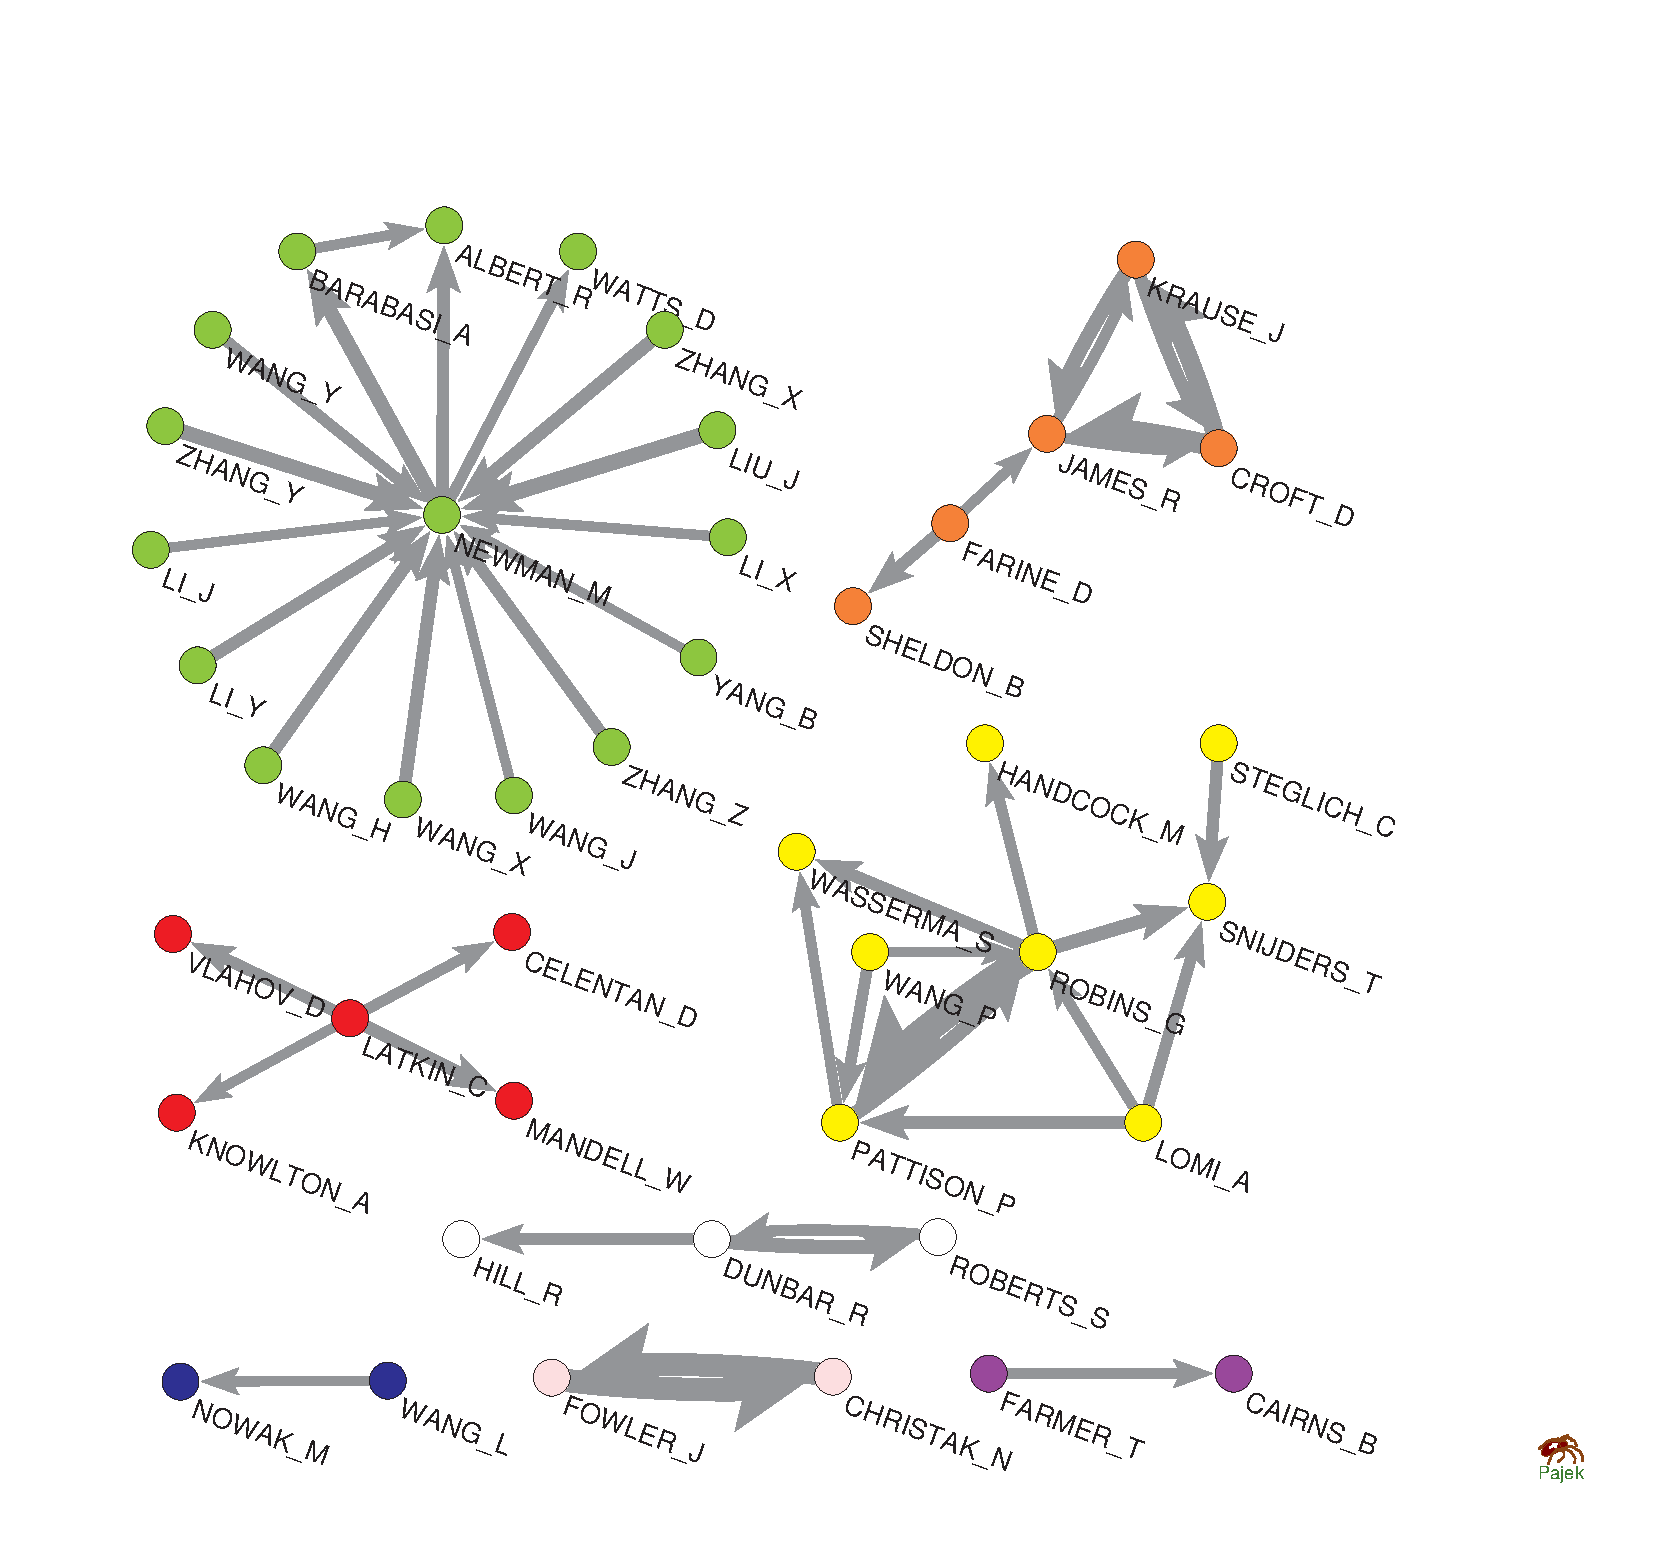
\includegraphics[width=70mm, viewport=55 45 675 655, clip=]{CiteA_43.pdf}
\end{center}

\end{frame}


\begin{frame}[fragile]
\frametitle{Citation among authors\\ \normalsize self-citation from CiteAn net}

\tiny
\begin{center}
\begin{tabular}{c|l|l|l|c|l|l|l|} 
\# &	Author & Value &	\% &  \# &	Author& Value & \% \\ \hline 
1&	TANG\_J&	9.786&	0.025&	26&	FALOUTSO\_C&	8.169&	0.014\\
2&	FARINE\_D&	9.778&	0.074&	27&	HANSON\_B&	8.091&	0.041\\
3&	PENTLAND\_A&	9.746&	0.016&	28&	SUEUR\_C&	8.025&	0.092\\
4&	MARATHE\_M&	9.528&	0.034&	29&	FRANK\_K&	7.995&	0.062\\
5&	ZENOU\_Y&	9.466&	0.077&	30&	LI\_X&	7.966&	0.020\\
6&	EVERETT\_M&	9.342&	0.012&	31&	MORENO\_M&	7.724&	0.034\\
7&	KRAUSE\_J&	9.035&	0.022&	32&	THELWALL\_M&	7.698&	0.033\\
8&	CHEN\_H&	8.975&	0.032&	33&	SHEN\_X&	7.679&	0.039\\
9&	BERKMAN\_L&	8.949&	0.007&	34&	KENNEDY\_A&	7.619&	0.070\\
10&	POTTERAT\_J&	8.899&	0.027&	35&	GARLAND\_S&	7.606&	0.087\\
11&	MORRIS\_M&	8.861&	0.025&	36&	ZHANG\_D&	7.586&	0.041\\
12&	KAZIENKO\_P&	8.802&	0.067&	37&	NOWAK\_M&	7.554&	0.021\\
13&	SHEN\_H&	8.799&	0.049&	38&	MAGLIANO\_L&	7.542&	0.051\\
14&	LIU\_J&	8.763&	0.034&	39&	BONACICH\_P&	7.540&	0.020\\
15&	XU\_Q&	8.667&	0.085&	40&	LU\_R&	7.458&	0.045\\
16&	TUCKER\_J&	8.496&	0.061&	41&	WANG\_J&	7.414&	0.023\\
17&	SKVORETZ\_J&	8.481&	0.056&	42&	WANG\_L&	7.345&	0.038\\
18&	THAI\_M&	8.453&	0.068&	43&	SAITO\_K&	7.335&	0.055\\
19&	BATAGELJ\_V&	8.421&	0.032&	44&	CHEN\_W&	7.245&	0.012\\
20&	MUTH\_S&	8.382&	0.026&	45&	FERRARI\_E&	7.209&	0.038\\
21&	MARTINEZ\_M&	8.313&	\textbf{0.141}&	46&	COHEN\_S&	7.202&	0.010\\
22&	LITWIN\_H&	8.297&	0.052&	47&	RYAN\_L&	7.193&	0.080\\
23&	STANTON\_N&	8.250&	\textbf{0.216}&	48&	MEYBODI\_M&	7.175&	\textbf{0.314}\\
24&	TUREL\_O&	8.227&	\textbf{0.161}&	49&	KIMURA\_M&	7.139&	0.053\\
25&	ABDELZAH\_T&	8.176&	0.085&	50&	KIM\_H&	7.121&	0.037\\
\end{tabular} 
\end{center}

\end{frame}

\begin{frame}[fragile]
\frametitle{Citation among authors\\ \normalsize Main island from CiteAn net}

\begin{center}
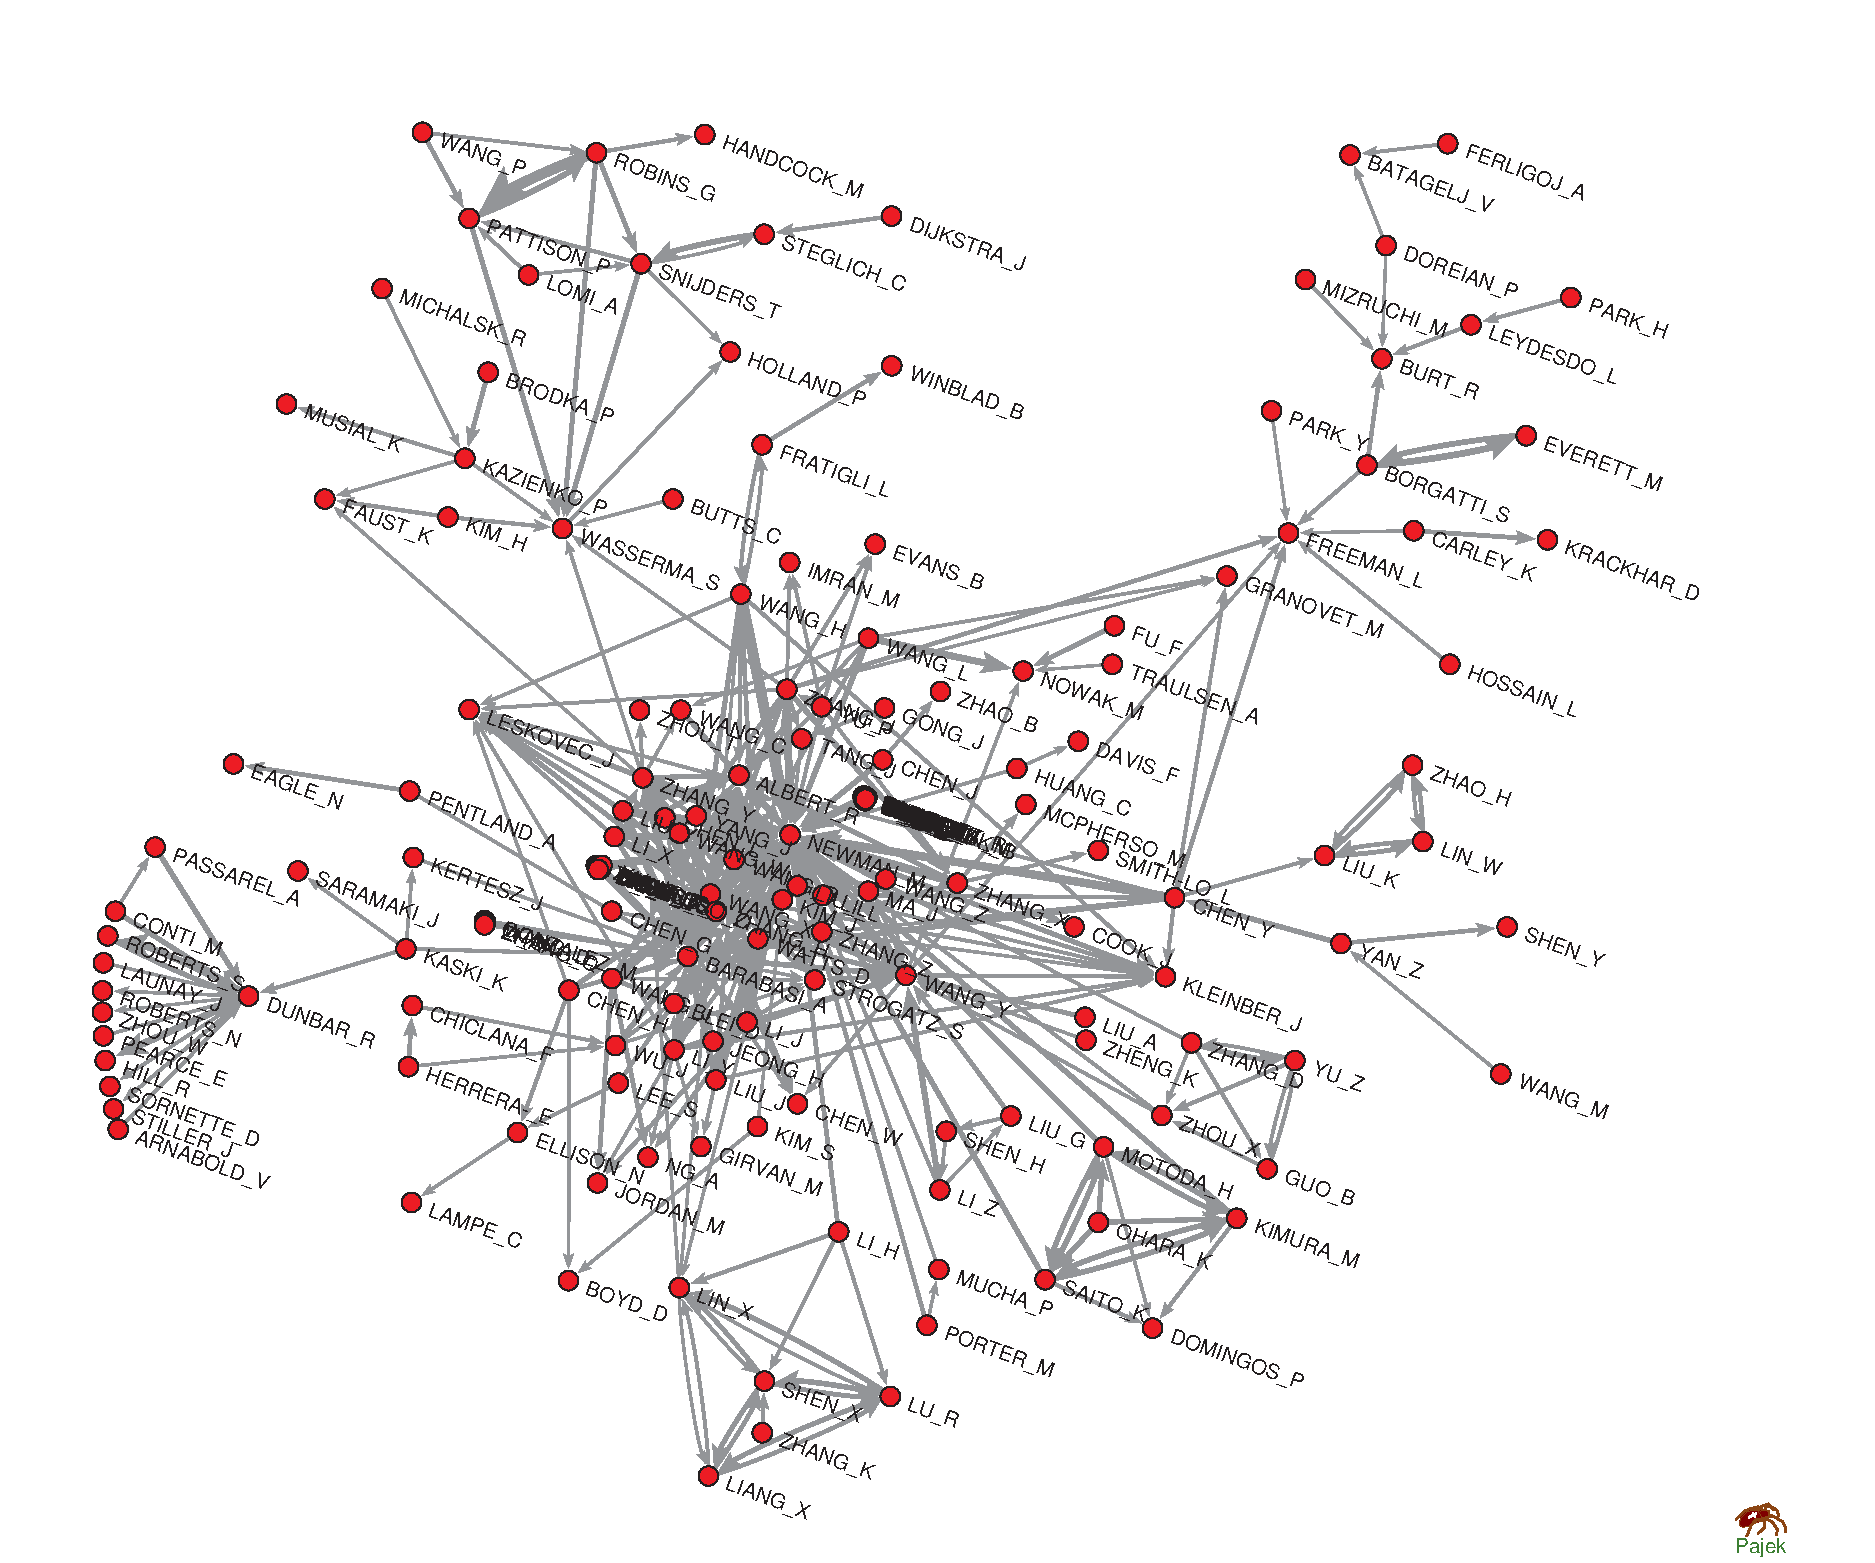
\includegraphics[width=80mm, viewport = 37 15 820 700, clip=]{CiteAmIsl.pdf}
\end{center}

\end{frame}

\begin{frame}[fragile]
\frametitle{Citation among journals\\ \normalsize CiteJ and CiteJn nets}

\footnotesize
Networks takes into account citations from papers published in journal \textit{i} to papers published in journal \textit{j}, which appeared in the works included into the \textbf{WJr} network. In the obtained network, the value of weight of the element [u,v] is equal to the \textbf{absolute number of citations} from journal $i$ to journal $j$. \smallskip

\[ \mathbf{CiteJ} = (\mathbf{WJr}) ^ T * \mathbf{CiteR} * \mathbf{WJr} \] 

Line weights take into account \textit{fractional} contribution of citations from papers published in journal $i$ to papers published in journal $j$. \medskip 

\[ \mathbf{CiteJn} = (\mathbf{WJr}) ^ T * n(\mathbf{CiteR}) * \mathbf{WJr} \]  


\end{frame}

\begin{frame}[fragile]
\frametitle{Citation among journals\\ \normalsize self-citation from CiteJ net}

\renewcommand{\arraystretch}{0.95}
\footnotesize
\begin{center}
\begin{tabular}{c|l|l} 
 Rank       &        Value   & Id		    \\ \hline 
         1  &    4443   & SOC NETWORKS		    \\
         2  &    2058   & COMPUT HUM BEHAV	    \\
         3  &     569   & PHYSICA A		    \\
         4  &     429   & PHYS REV E		    \\
         5  &     382   & LECT NOTES COMPUT SC	    \\
         6  &     339   & CYBERPSYCHOL BEHAV	    \\
         7  &     328   & SOC SCI MED		    \\
         8  &     315   & AM J SOCIOL		    \\
         9  &     303   & PLOS ONE		    \\
        10  &     258   & ANIM BEHAV		    \\
        11  &     246   & SCIENTOMETRICS	    \\
        12  &     232   & J MED INTERNET RES	    \\
        13  &     226   & P NATL ACAD SCI USA	    \\
        14  &     209   & ORGAN SCI		    \\
        15  &     194    & BEHAV ECOL SOCIOBIOL	     \\ \hline 
\end{tabular} 
\end{center}

\end{frame}

\begin{frame}[fragile]
\frametitle{Citation among journals\\ \normalsize authors with largest line weights from CiteJ net}

\begin{center}
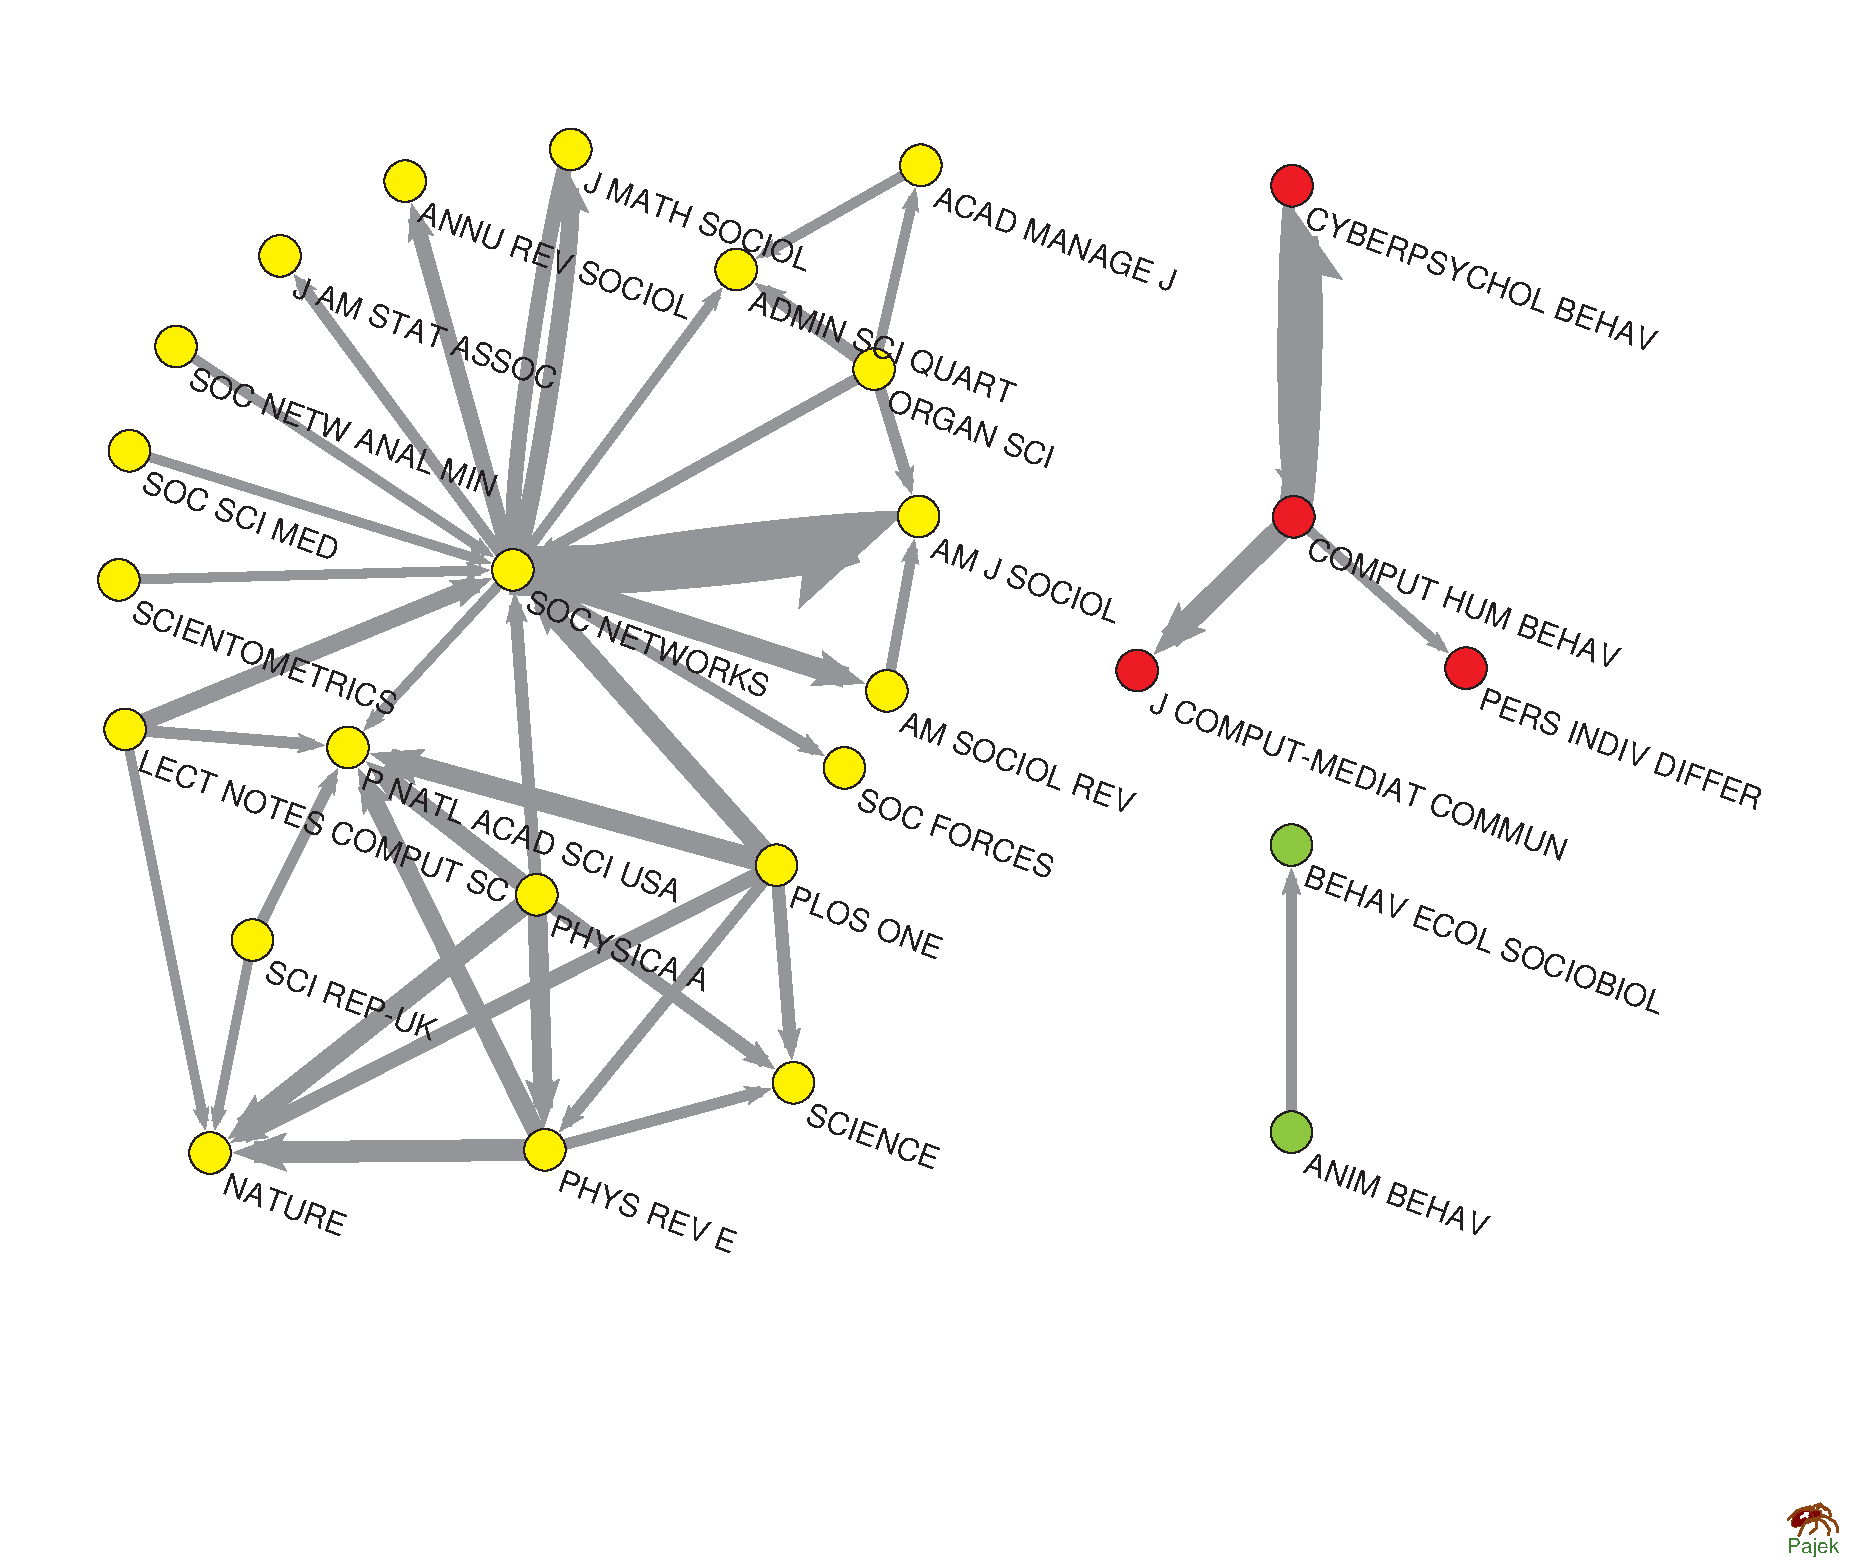
\includegraphics[width=\textwidth]{JCiJ_27.pdf}
\end{center}

\end{frame}

\begin{frame}[fragile]
\frametitle{Citation among journals\\ \normalsize self-citation from CiteJn net}

\renewcommand{\arraystretch}{0.95}
\tiny
\begin{center}
\begin{tabular}{p{0.1cm}|p{0.5cm}|p{0.3cm}|p{2.7cm}|p{0.1cm}|p{0.5cm}|p{0.3cm}|p{2.6cm}|} 
\# &	Value& \% &	Journal &  \# &	Value& \% & Journal \\ \hline 
1 &	\textbf{355.65}&	\textbf{0.34}&	SOC NETWORKS&	16&	       18.35 &    0.17	  &     ANIM BEHAV\\
2 &	\textbf{168.39}&	0.22&	COMPUT HUM BEHAV&	17&    17.03 & 	  0.12	  &     AIDS BEHAV\\
3 &	\textbf{122.57}&	0.09&	LECT NOTES COMPUT SC&	18&    16.03 & 	  0.19	  &     AM J COMMUN PSYCHO \\
4 &	57.75&	0.13&	PHYSICA A&	19&	       14.87 &	  0.10	  &     INFORM SCI\\
5 &	43.00&	0.14&	SOC SCI MED&	20&	       14.14 &	  0.14	  &     KNOWL-BASED SYST\\
6 &	42.18&	\textbf{0.24}&	J MED INTERNET RES&	21&    12.64 &	  0.19	  &     PROF INFORM\\
7 &	41.49&	0.21&	CYBERPSYCHOL BEHAV&	22&    12.35 & 	 \textbf{0.23}	  &     COMUNICAR\\
8 &	33.16&	0.05&	PLOS ONE&	23&	       12.00 & 	  0.18	  &     BEHAV ECOL SOCIOBI \\
9 &	32.93&	0.11&	PHYS REV E&	24&	       11.87 & 	  \textbf{0.25}	  &     AM J EPIDEMIOL\\
10 &	30.22&	0.13&	SCIENTOMETRICS&	25&	       11.01 & 	  0.11	  &     DECIS SUPPORT SYST \\
11 &	24.16&	0.14&	P NATL ACAD SCI USA&	26&    10.58 & 	  0.14	  &     J ETHN MIGR STUD\\
12 &	23.15&	\textbf{0.26}&	AM J SOCIOL&	27&	       10.43 & 	  0.13	  &     COMPUT EDUC\\
13 &	20.04&	0.05&	LECT NOTES ARTIF INT&	28&    10.31 & 	  0.18	  &     SEX TRANSM DIS\\
14 &	19.31&	0.12&	EXPERT SYST APPL&	29&    10.19 & 	 \textbf{0.28}	  &     NATURE\\
15 &	18.77&	0.14&	NEW MEDIA SOC&	30&	       9.85 & 	  0.09	  &     ORGAN SCI\\ \hline 
\end{tabular} 
\end{center}

\end{frame}

\begin{frame}[fragile]
\frametitle{Citation among journals\\ \normalsize Main island from CiteJn net}

\begin{center}
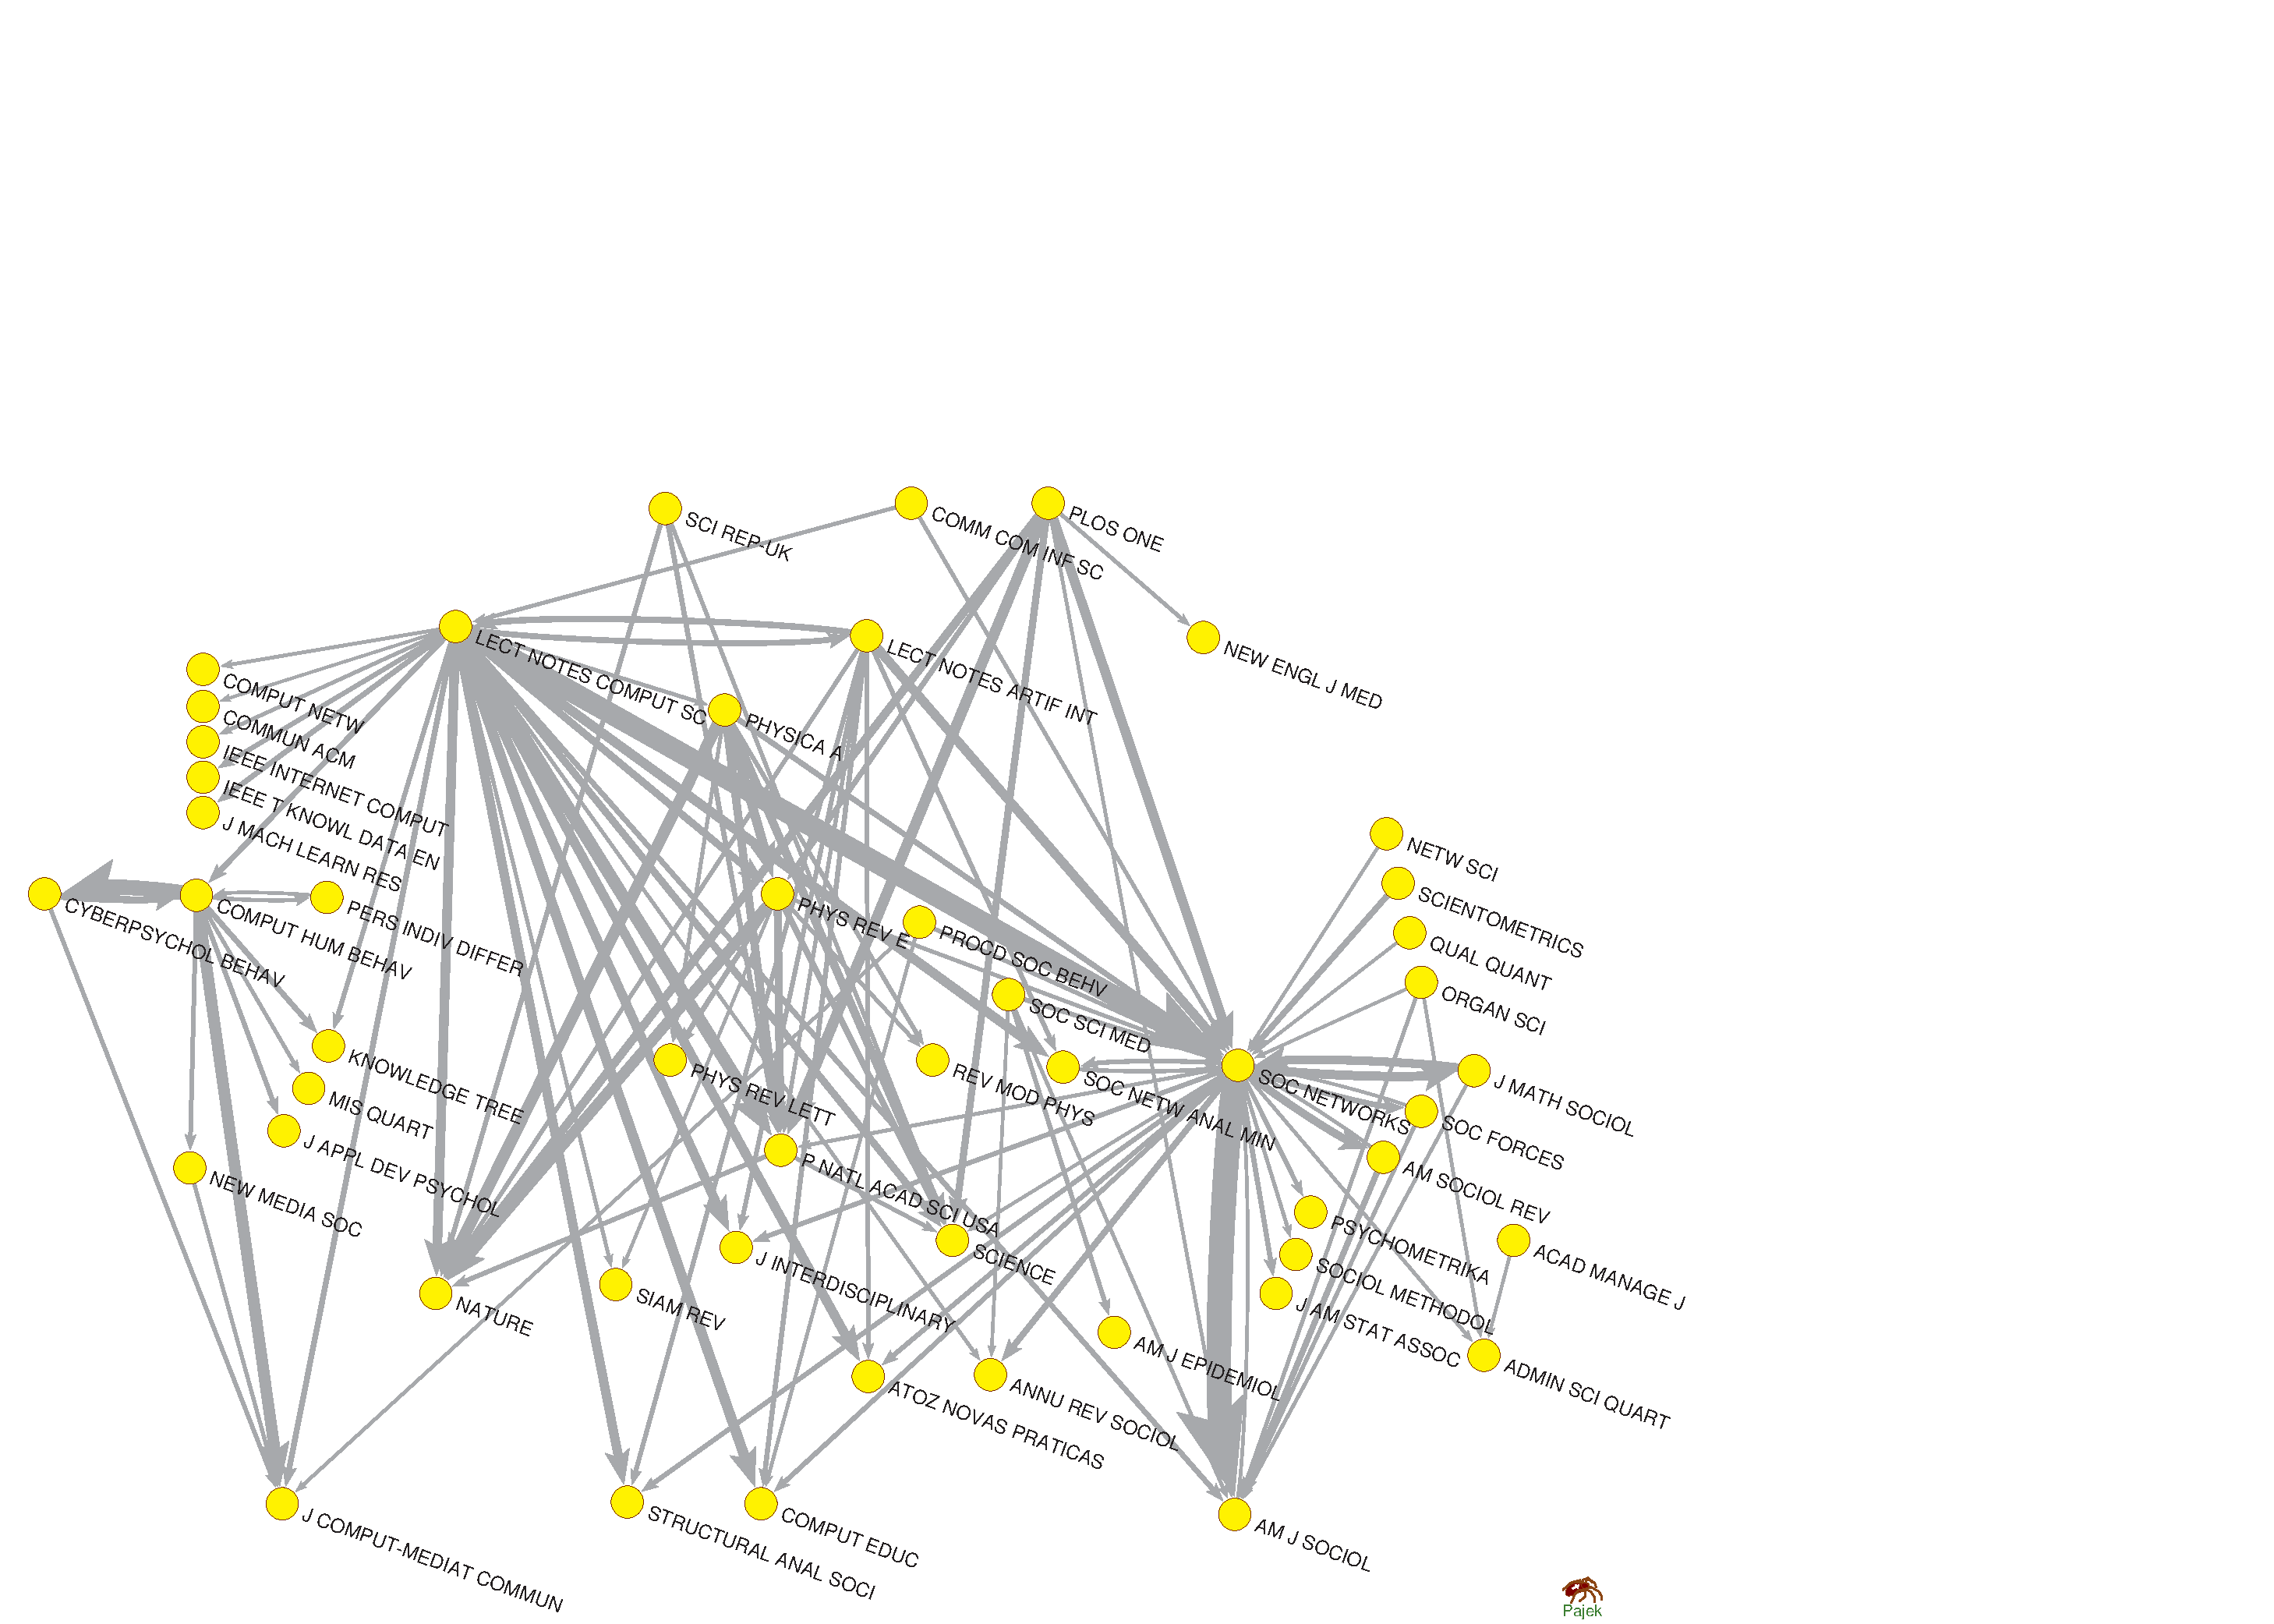
\includegraphics[width=100mm,viewport=10 0 1042 708,clip=]{JJsfmain2.pdf}
\end{center}

\end{frame}

\begin{frame}[fragile]
\frametitle{Citation among journals\\ \normalsize Pairs of journals with largest line weights from CiteJn net}

\renewcommand{\arraystretch}{0.83}
\tiny
\begin{center}
\begin{tabular}{c|l|p{3cm}|p{3cm}}
\# &	value &	from journal  &	to journal \\  \hline 
1&	8,1&	IEEE GLOB COMM CONF&	IEEE INFOCOM SER\\
2&	6,26&	HIST COMUN SOC&	COMUNICAR\\
3&	4,63&	J YOUTH ADOLESCENCE&	J RES ADOLESCENCE\\
4&	4,44&	INT J GERIATR PSYCH&	J PSYCHIAT RES\\
5&	4,38&	INT MIGR&	INT MIGR REV\\
6&	4,31&	J BUS ETHICS&	ACAD MANAGE REV\\
7&	3,99&	DEMOGR RES&	DEMOGRAPHY\\
8&	3&	J INTELL FUZZY SYST&	J APPL MATHE COMPUT\\
9&	3&	J INT DEV&	TROP MED INT HEALTH\\
10&	3&	PERVASIVE MOB COMPUT&	INT CONF PERVAS COMP\\
11&	2,78&	J CONSTR ENG M&	J CONSTR ENG M ASCE\\
12&	2,68&	PHYS EDUC RES CONF&	PHYS REV SPEC TOP-PH\\
13&	2,59&	ENERGY RES SOC SCI&	ENERG POLICY\\
14&	2,5&	INT P ECON DEV RES&	TECHNOVATION\\
15&	2,37&	COMPUT ASSIST LANG L&	LANG LEARN TECHNOL\\
16&	2,33&	INFORM SOC-ESTUD&	PERSPECT CIENC INF\\
17&	2,33&	WORLD DEV&	ECON J\\
18&	2,31&	J PEACE RES&	J CONFLICT RESOLUT\\
19&	2,22&	HEALTH RES POLICY SY&	HEALTH POLICY PLANN\\
20&	2,1&	SEX HEALTH&	INT J STD AIDS\\
21&	2&	REV LAT COMUN SOC&	PALABRA CLAVE\\
22&	2&	J RETAIL CONSUM SERV&	AUSTRALAS MARK J\\
23&	2&	ETHN DIS&	HEART LUNG\\
24&	2&	IEEE INT SYMP INFO&	IEEE T INFORM THEORY\\
25&	2&	REV BRAS ENFERM&	REV LAT-AM ENFERM\\ \hline 
\end{tabular}
\end{center}

\end{frame}

%******************************************************************************
\subsection{Co-citation}  

\begin{frame}[fragile]
\frametitle{Bibliographic coupling \\ \normalsize Jaccard biCo, JCoj and ACoj nets}

\footnotesize
\[ \mathbf{biCo} = \mathbf{CiteR} * (\mathbf{CiteR}) ^ T \]  

Normalization create networks $n(\mathbf{WJr})$ and $n(\mathbf{WAr})$ where the weight of each arc is divided by the sum of weights of all arcs having the same initial node (journal or author) as this arc (outdegree of a node).

 Line weights in the obtained networks take into account \textit{fractional} similarity of journals $i$ and $j$, or authors $u$ and $v$. 

\[ \mathbf{JCoj} = n(\mathbf{WJr}) ^ T * \mathbf{biCoj} * n(\mathbf{WJr}) \]  

\[ \mathbf{ACoj} = n(\mathbf{WAr}) ^ T * \mathbf{biCoj} * n(\mathbf{WAr}) \]  

The values of links from biCoj are redistributed in JCoj and ACoj. 

	\[ \sum_{e \in E(\mathbf{JCoj})} \mathbf{JCoj}[e] = \sum_{e \in E(\mathbf{biCoj})} \mathbf{biCoj}[e] \] 

The total sum of link weights is preserved.

\end{frame}

\begin{frame}[fragile]
\frametitle{Bibliographic coupling \\ \normalsize Jaccard biCo, JCoj and ACoj nets}
\footnotesize
The produced Jaccard network \textbf{biCo} contained a large number of links -- 62.079.457, -- and the computation of networks \textbf{JCoj} and \textbf{ACoj} would be quite time consuming. \medskip 

The desision was made to make a line cut in the Jaccard \textbf{biCo} at the level 0.085, and then use the obtained network for the multiplication with WJsr and WAsr networks, respectively.  \medskip 

Obtained \textbf{biCo} network contained 70.792 works and 13.208.451 linkes. After multiplication, we got \textbf{JCoj} network with 8.943 nodes and 4.966.617 arcs, and \textbf{ACoj} network with 93.011 nodes and 127.220.243 arcs. In both obtained networks, the loops were deleted, the bidirected arcs were converted to edges (with summation of values) before the further analysis. \medskip 

\end{frame}

\begin{frame}[fragile]
\frametitle{Bibliographic coupling \\ \normalsize Co-citation among journals JCoj}

\begin{center}
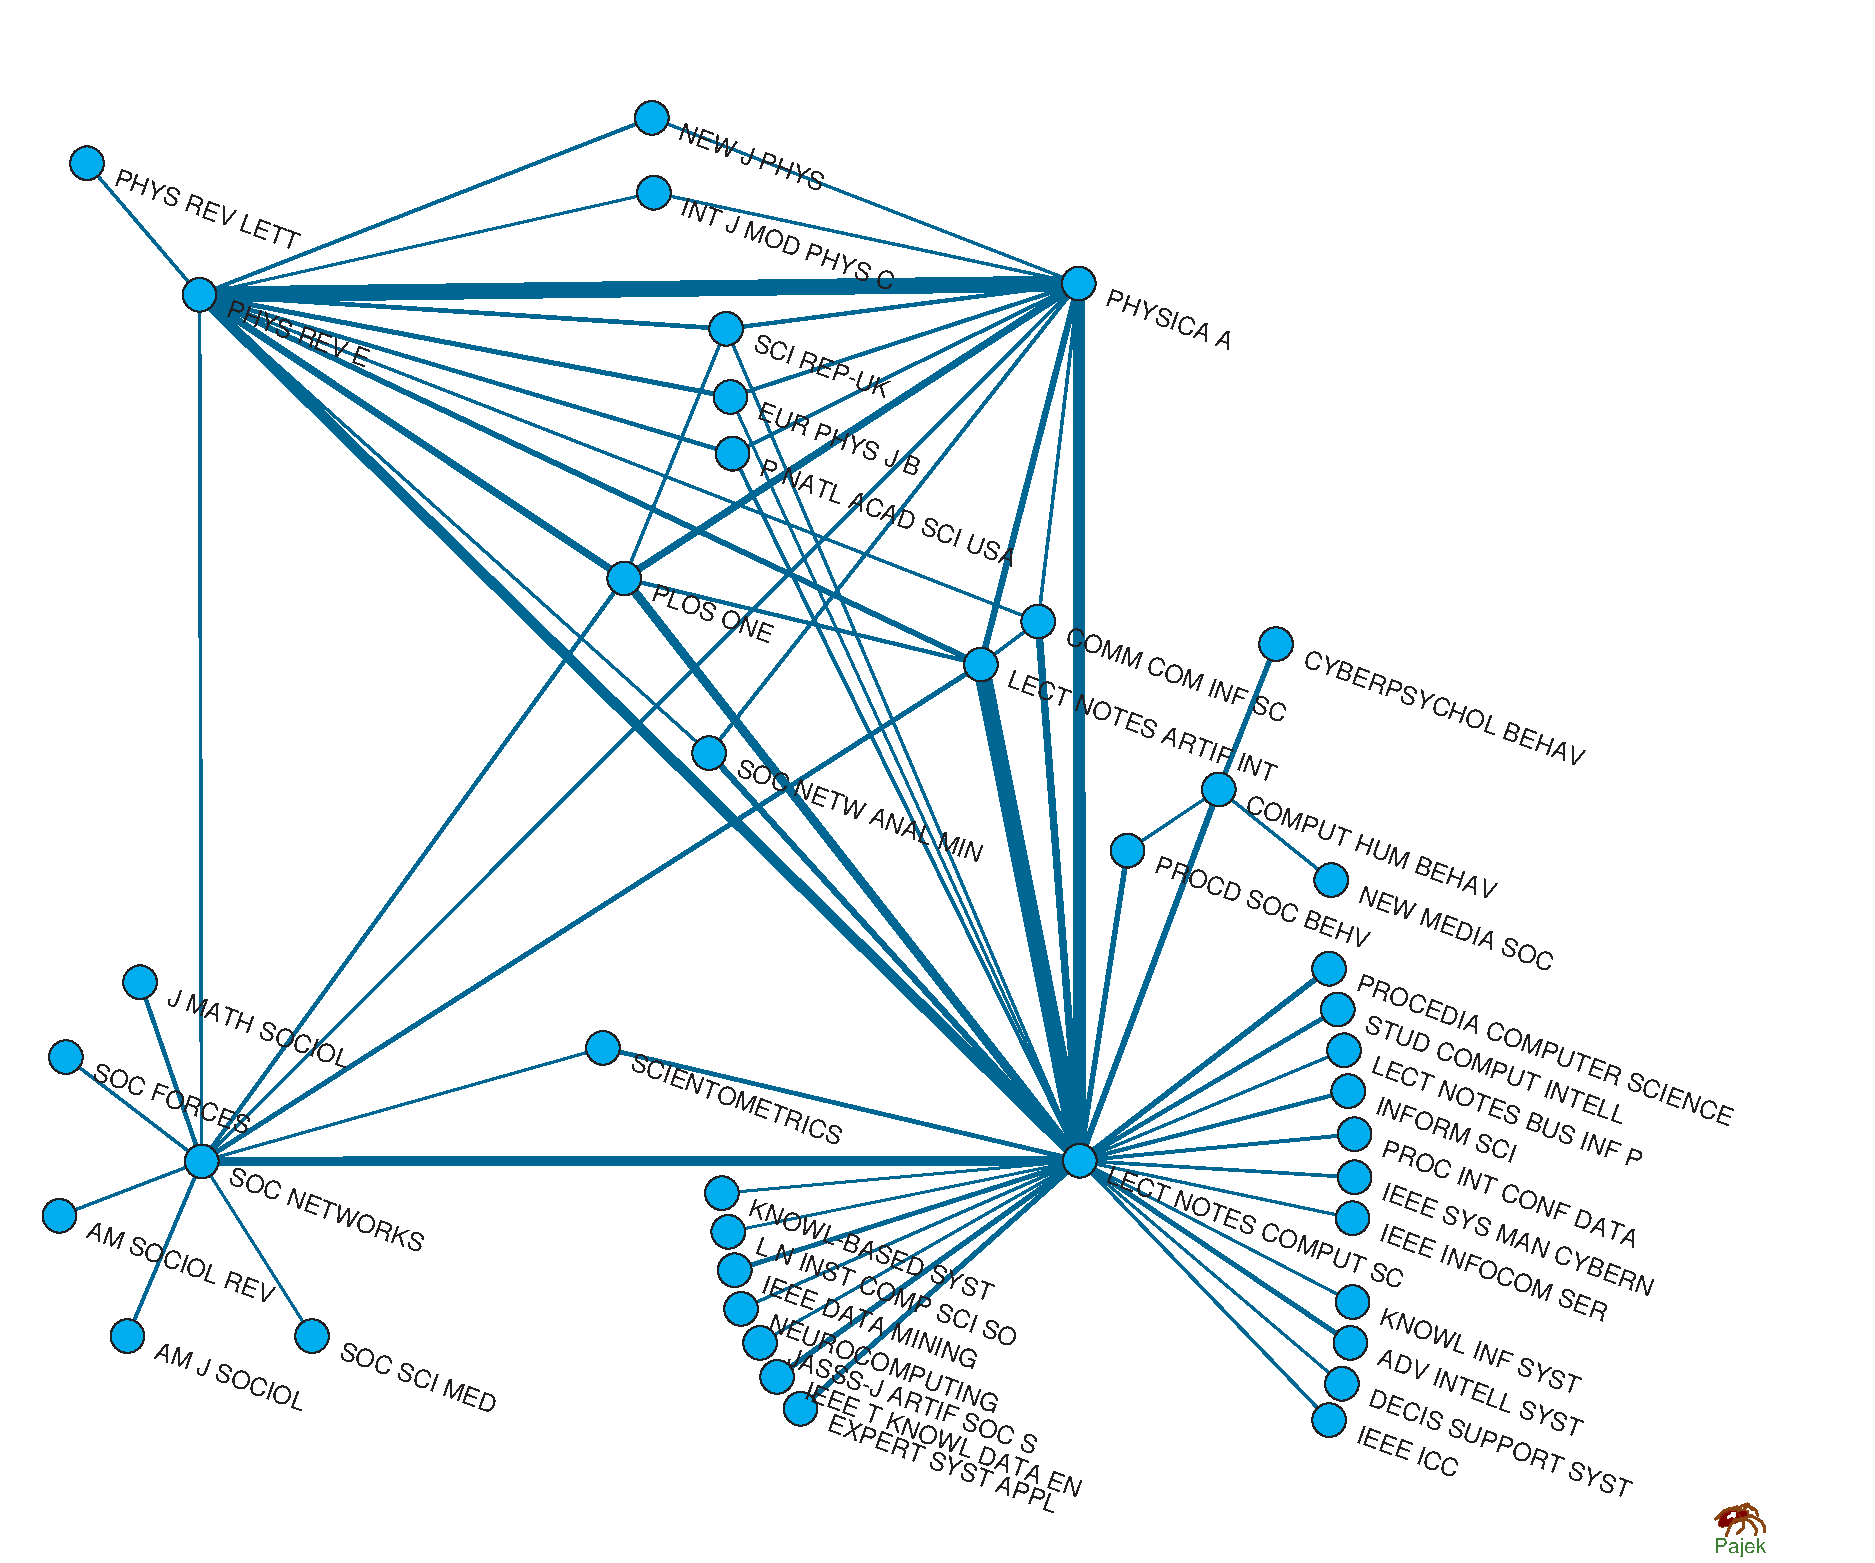
\includegraphics[width=80mm, viewport = 14 0 854 706, clip=]{JacJou.pdf}
\end{center}

\end{frame}


\begin{frame}[fragile]
\frametitle{Bibliographic coupling \\ \normalsize Co-citation among authors ACoj}

\begin{center}
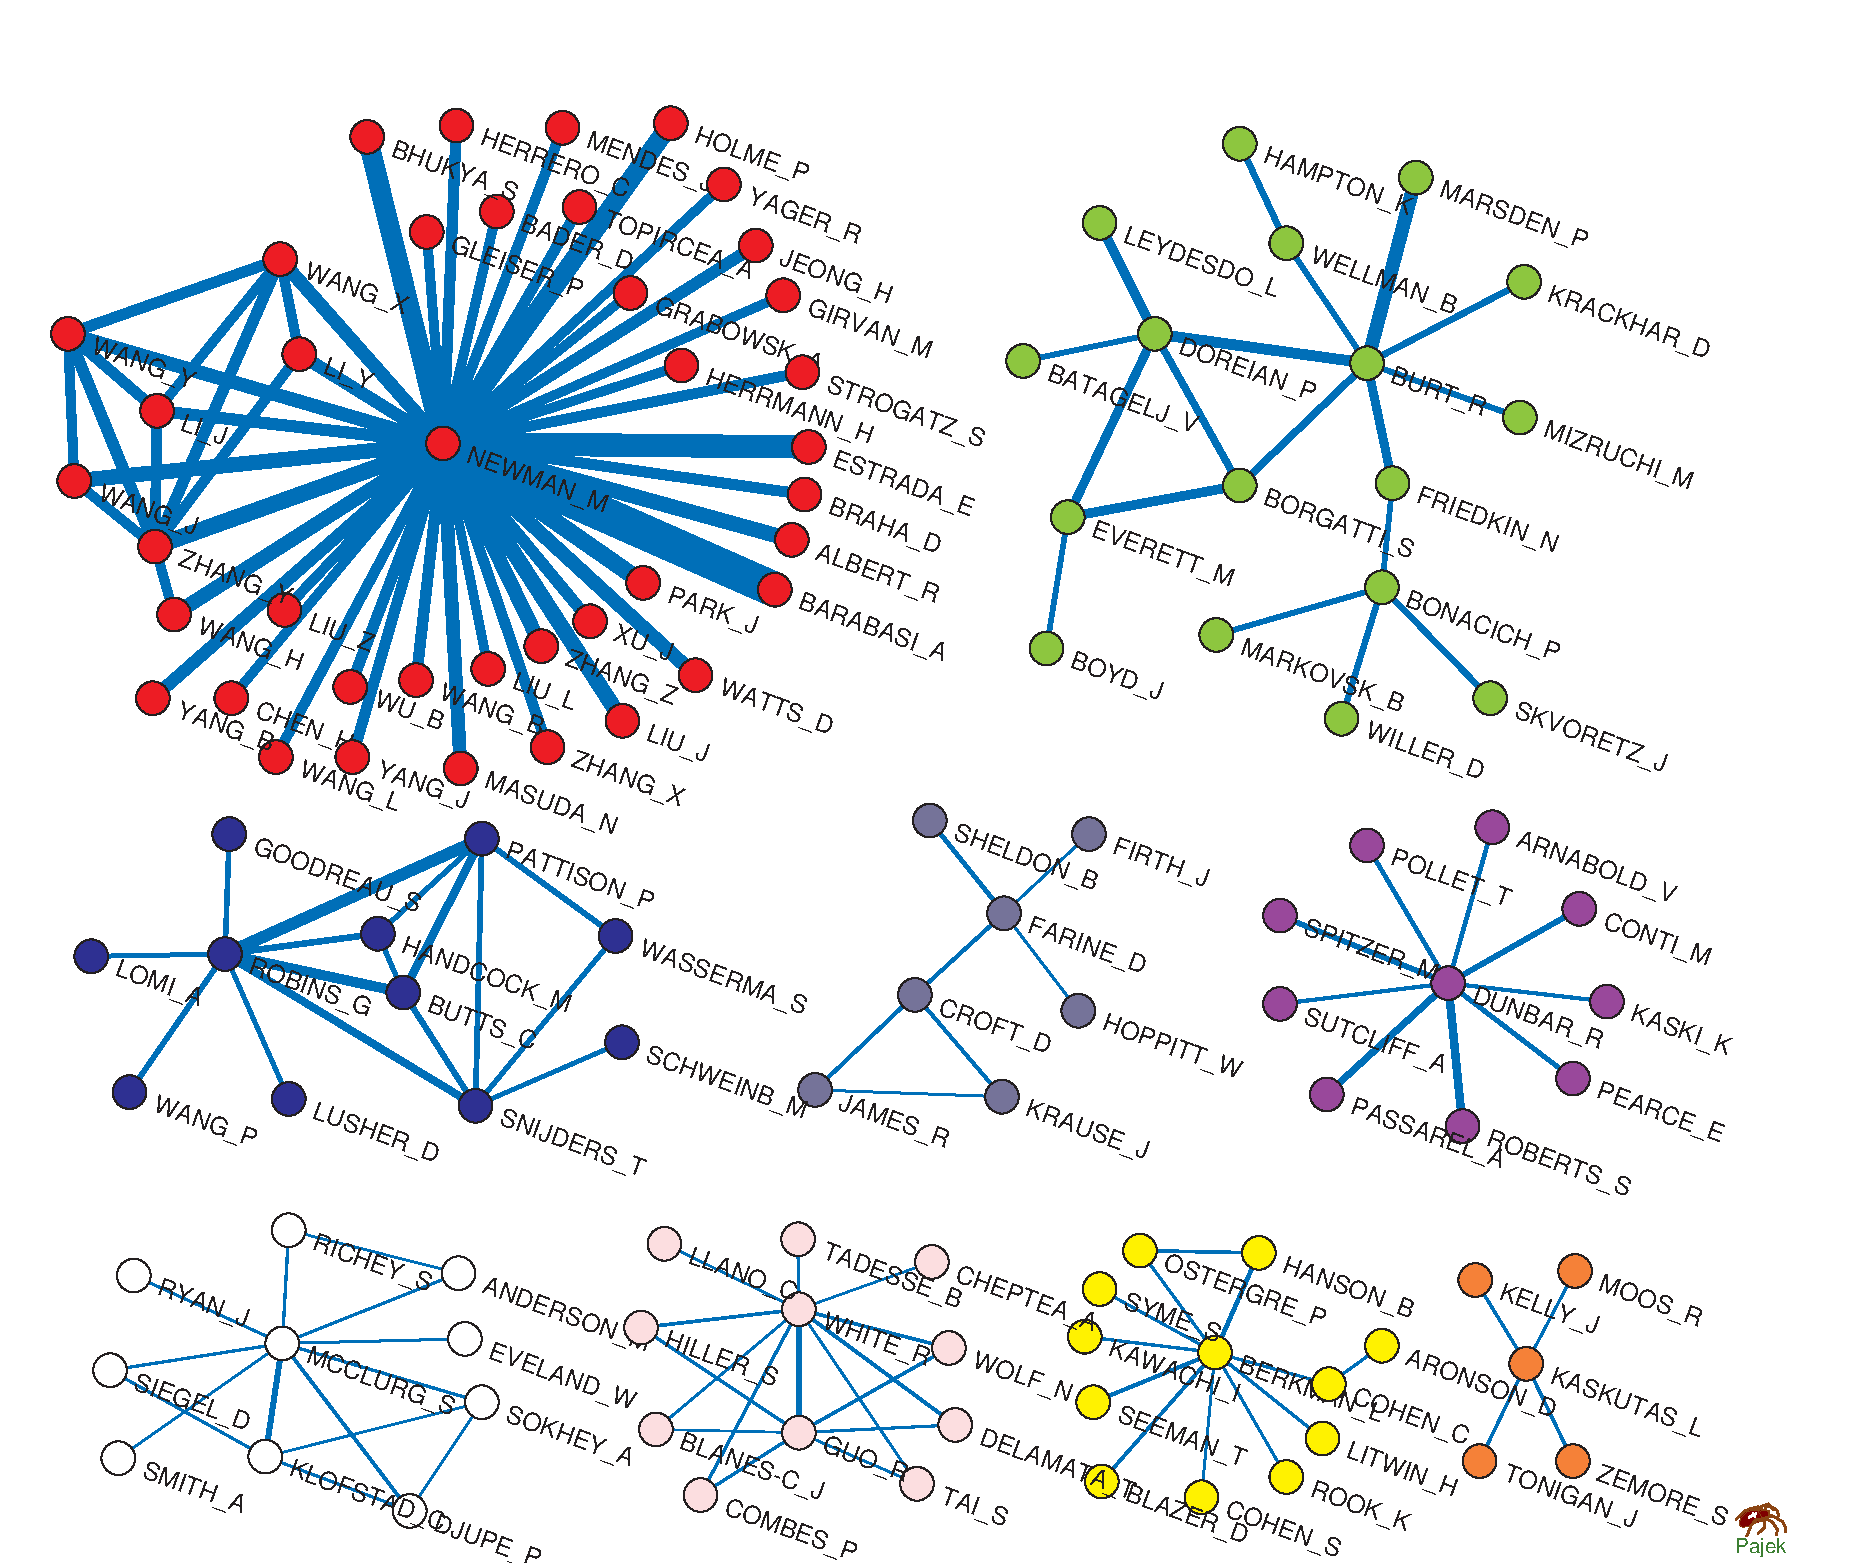
\includegraphics[width=80mm, viewport = 15 0 830 705, clip=]{JacAu.pdf}
\end{center}

\end{frame}

%******************************************************************************
\subsection{Keywords co-occurence}  

\begin{frame}[fragile]
\frametitle{Keywords co-occurence \\ \normalsize KK net}
\small 

\[ \mathbf{KKn} = n(\mathbf{WK})^T * n(\mathbf{WK}) \]
where 
\[ n(\mathbf{WK})[w,k] = \frac {\mathbf{WK}[w,k]}{\textrm{max}(1,outdeg(w))}\]
\medskip

\medskip 
\small
Fractional approach:\smallskip 

The fractional contribution of each complete subgraph in $KKn$ is 1 -- all works are contributing equally (the works with large number of keywords are not overrepresented). 

The weight of the edges between the nodes (keywords) is equal to the \textit{fractional} co-occurence of keywords $i$ and $j$ in the same works.

\end{frame}

\begin{frame}[fragile]
\frametitle{Keywords co-occurence \\ \normalsize KK net Main island}
\small 
\begin{center}
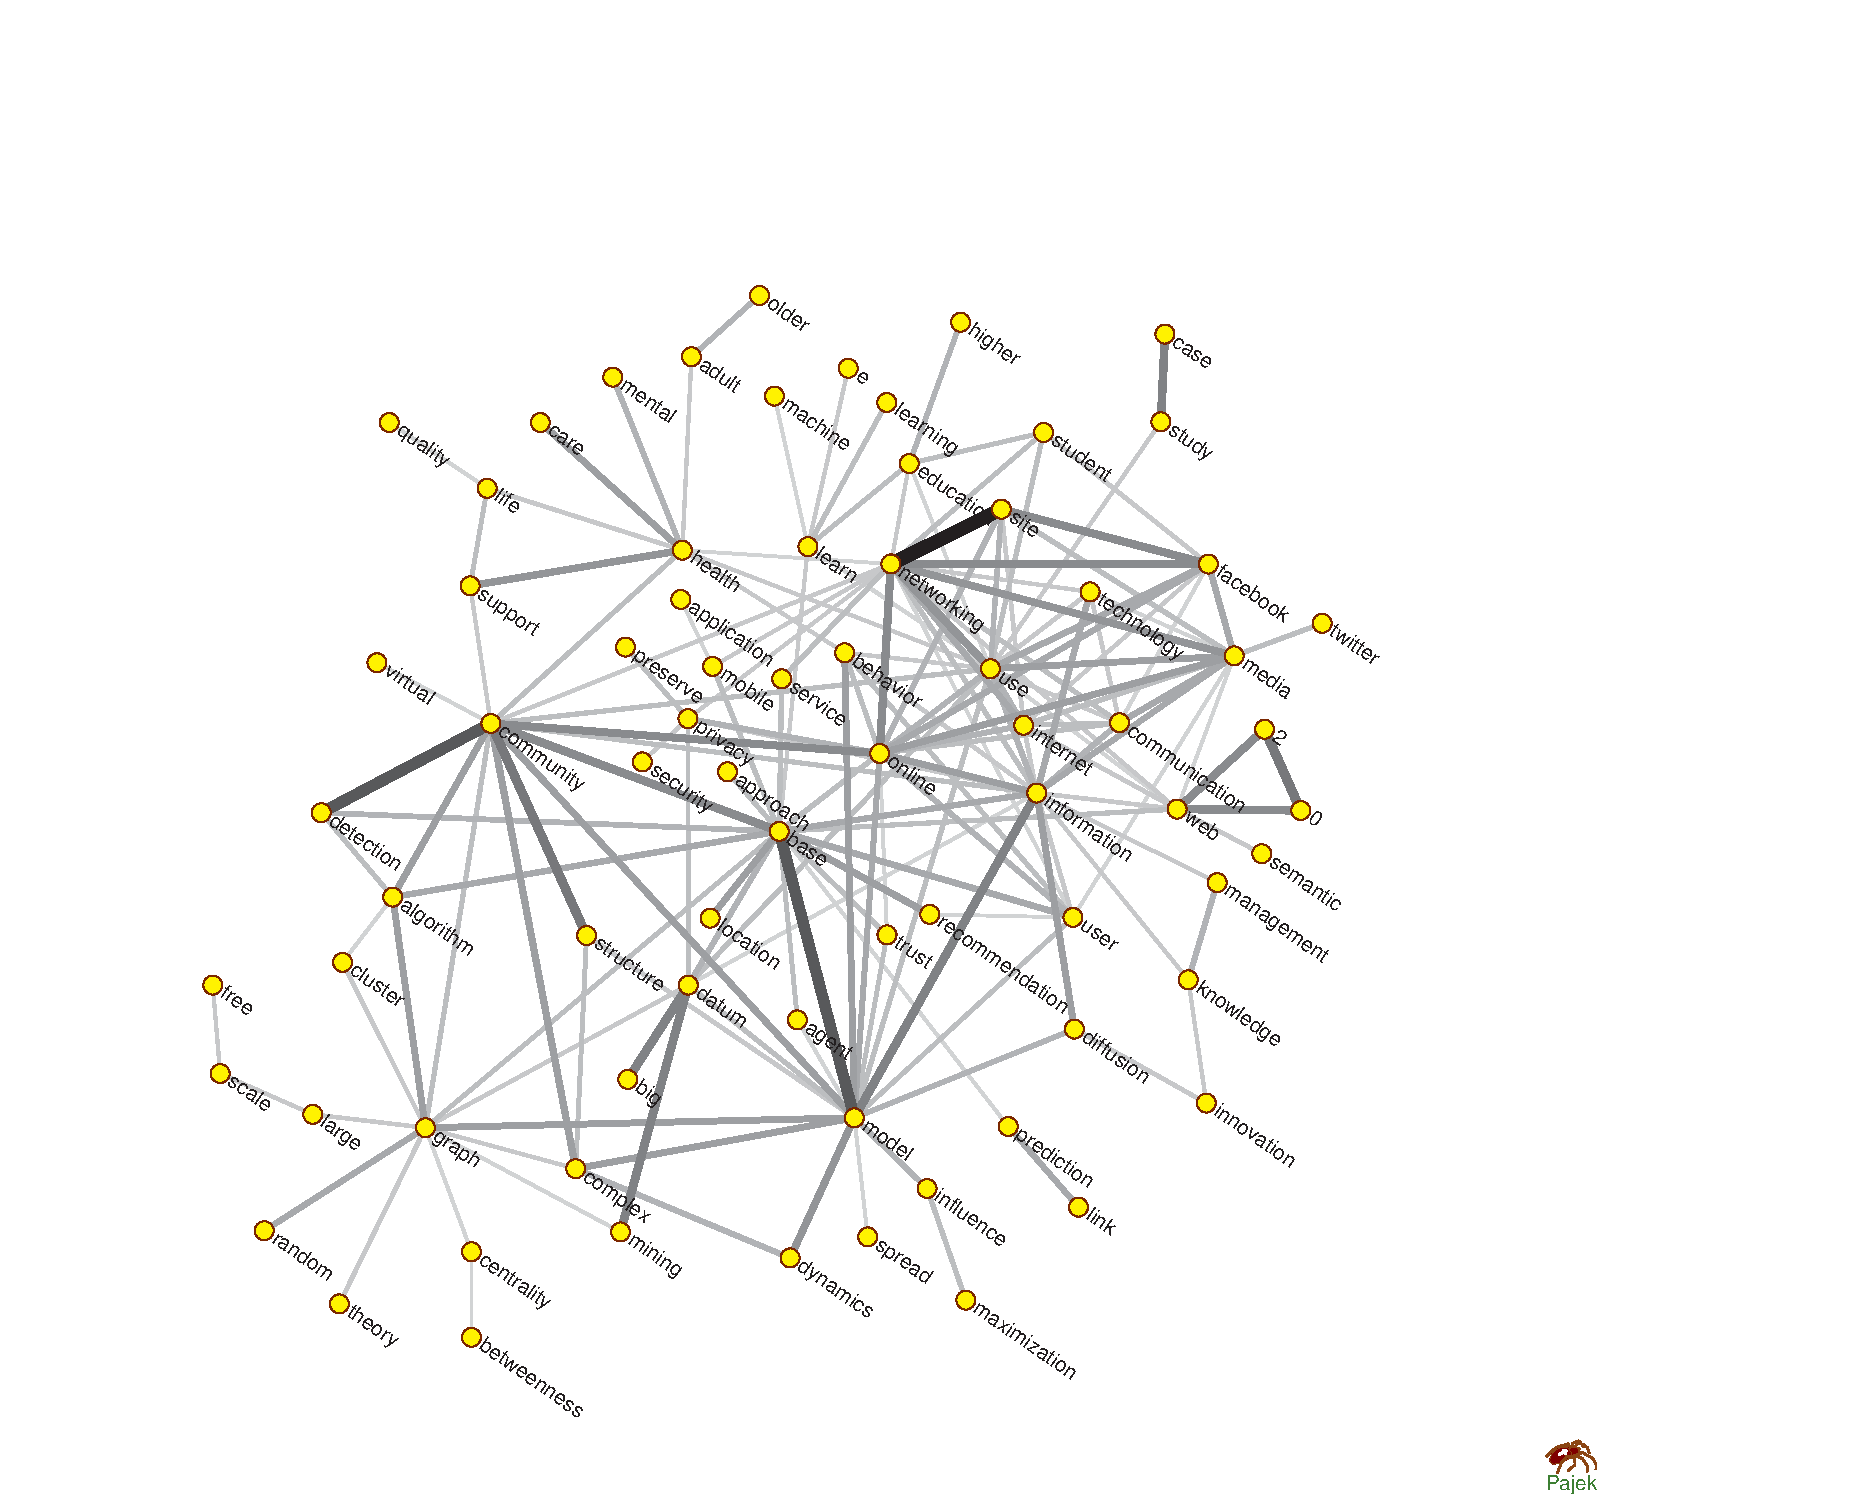
\includegraphics[width=83mm, viewport = 19 35 670 590, clip=]{KKmain.pdf}
\end{center}

\end{frame}

\section{Temporal}  
\subsection{Networks}

\begin{frame}[fragile]
\frametitle{Temporal networks\\ \normalsize }
\small
Using the \textbf{Temporal quantities approach} [Batagelj and Praprotnik, 2016] and Python packages \textbf{Nets.py} and \textbf{TQ.py}, out of the reduced networks \textbf{WAr, WJr, WKr}, and \textbf{CiteR} we constructed the set of temporal networks of two types -- \textit{instantaneous} (with values given per each year) and \textit{cumulative} (with cumulative values over the years) in \texttt{.json} format. These are the networks \textbf{WAins, WAcum, WJins, WJcum, WKrins, WKcum}, and \textbf{CiteIns, CiteCum}. \medskip 

These temporal networks were used for construction of other \textbf{obtained} temporal networks.

\end{frame} 

\begin{frame}[fragile]
\frametitle{Temporal networks\\ \normalsize }
\small
Example of node with temporal quantities -  \textit{instantaneous}: \medskip

['NEWMAN\_M', [(1894, 1999, 0), (1999, 2000, 2), (2000, 2001, 4), (2001, 2002, 9), (2002, 2003, 10), (2003, 2004, 9), (2004, 2005, 15), (2005, 2006, 7), (2006, 2007, 13), (2007, 2008, 4), (2008, 2009, 1), (2009, 2010, 2), (2010, 2011, 3), (2011, 2016, 0), (2016, 2017, 2), (2017, 2019, 0)]] \medskip

Example of node with temporal quantities -  \textit{cumulative}: \medskip

['NEWMAN\_M', [(1894, 1999, 0), (1999, 2000, 2), (2000, 2001, 6), (2001, 2002, 15), (2002, 2003, 25), (2003, 2004, 34), (2004, 2005, 49), (2005, 2006, 56), (2006, 2007, 69), (2007, 2008, 73), (2008, 2009, 74), (2009, 2010, 76), (2010, 2011, 79), (2011, 2016, 79), (2016, 2017, 81), (2017, 2019, 81)]]


\end{frame} 

\subsection{Authors}

\begin{frame}[fragile]
\frametitle{Number of publications for certain authors \\ \normalsize Indegree of WAins network }
\begin{center}
\centerline{
\includegraphics[width=0.31\textwidth]{Doreian.pdf} 
\includegraphics[width=0.31\textwidth]{Wellman.pdf} 
\includegraphics[width=0.31\textwidth]{Burt.pdf}} 
\centerline{
\includegraphics[width=0.31\textwidth]{Snijders.pdf} 
\includegraphics[width=0.31\textwidth]{Borgatti.pdf} 
\includegraphics[width=0.31\textwidth]{Valente.pdf}}
\centerline{
\includegraphics[width=0.31\textwidth]{Newman.pdf} 
\includegraphics[width=0.31\textwidth]{Barabasi.pdf}
\includegraphics[width=0.31\textwidth]{Wang.pdf}} 
\end{center}
\end{frame} 

\begin{frame}[fragile]
\frametitle{Number of publications for certain authors \\ \normalsize Indegree from WAcum network }

\centerline{
\includegraphics[width=0.45\textwidth]{Co_Latkin.pdf} 
\includegraphics[width=0.45\textwidth]{Co_Valente.pdf}}
\centerline{
\includegraphics[width=0.45\textwidth]{Co_Christakis.pdf} 
\includegraphics[width=0.45\textwidth]{Co_Pattison.pdf}}

\end{frame}  

\begin{frame}[fragile]
\frametitle{Collaboration networks CCn and CCtt \\ \normalsize Constructed from WAins and WAcum networks } 

\footnotesize 

\[ n(\mathbf{WAcum})[w,a] = \frac {\mathbf{WAcum}[w,a]}{\max(1,\textrm{outdeg}(w))}\]
then 
\[ \mathbf{CCn} = (\mathbf{WAcum}) ^ T * n(\mathbf{WAcum}), \]

The weight of the edges between the nodes (authors) is equal to the contribution of author $i$ to works, that he or she wrote together with author $j$. 

\[ n'(\mathbf{WAins})[w,a] = \frac {\mathbf{WAins}[w,a]}{\max(1,\textrm{outdeg}(w)-1)}\] 
then 
\[ \mathbf{CCtt} = n(\mathbf{WAins}) ^ T * n'(\mathbf{WAins}), \]

\footnotesize 
The weights of the edges between the nodes (authors) are equal to the total contribution of “strict collaboration” of authors $i$ and $j$ to works they wrote together.

\end{frame}  
 
\begin{frame}[fragile]
\frametitle{Collaborativenness indexes for certain authors \\ \normalsize from Collaboration network CCn  } 

\centerline{
\includegraphics[width=0.29\textwidth]{CI_Latkin.pdf} 
\includegraphics[width=0.29\textwidth]{CI_Valente.pdf} 
\includegraphics[width=0.29\textwidth]{CI_Christakis.pdf}}
\centerline{
\includegraphics[width=0.29\textwidth]{CI_Pattison.pdf} 
\includegraphics[width=0.29\textwidth]{CI_Wellman.pdf} 
\includegraphics[width=0.29\textwidth]{CI_Burt.pdf}}
\centerline{
\includegraphics[width=0.29\textwidth]{CI_Doreian.pdf}
\includegraphics[width=0.29\textwidth]{CI_Newman.pdf}}

\end{frame}   

\begin{frame}[fragile]
\frametitle{Input to collaboration for certain authors \\ \normalsize from Collaboration network CCtt } 

\centerline{
\includegraphics[width=0.31\textwidth]{Ct`_Pattison.pdf}
\includegraphics[width=0.31\textwidth]{Ct`_Doreian.pdf}
\includegraphics[width=0.31\textwidth]{Ct`_Snijders.pdf}}
\centerline{
\includegraphics[width=0.31\textwidth]{Ct`_Borgatti.pdf} 
\includegraphics[width=0.31\textwidth]{Ct`_Valente.pdf}
\includegraphics[width=0.31\textwidth]{Ct`_Christakis.pdf}}
\centerline{
\includegraphics[width=0.31\textwidth]{Ct`_Barabasi.pdf} 
\includegraphics[width=0.31\textwidth]{Ct`_Newman.pdf}}

\end{frame}   

\begin{frame}[fragile]
\frametitle{Citations among authors \\ \normalsize ACA and ACAn nets from WAins, WAcum and CiteIns nets} 

\[ \mathbf{ACA} = (\mathbf{WAins}) ^ T * \mathbf{CiteIns} * \mathbf{WAcum} \] 

The value of weight of the element $ACA[u,v]$ is equal to the \textbf{absolute number of citations} per year from works coauthored by $u$ to works coauthored by $v$. \smallskip

\[ \mathbf{ACAn} = (\mathbf{WAins}) ^ T * n(\mathbf{CiteIns}) * \mathbf{WAcum} \]  
where 
\[ n(\mathbf{CiteIns})[u,v] = \frac {\mathbf{CiteIns}[u,v]}{\max(1,\textrm{outdeg}(u))}\]

The value of element ACAn[u,v] is equal to the number of \textbf{fractional contribution} of citations per year from works coauthored by $u$ to works coauthored by $v$.\smallskip

\end{frame}   

\begin{frame}[fragile]
\frametitle{Self-citations among certain authors \\ \normalsize Loops from ACA network} 
\centerline{
\includegraphics[width=0.29\textwidth]{WellmanCiteA.pdf}
\includegraphics[width=0.29\textwidth]{ValenteCiteA.pdf} 
\includegraphics[width=0.29\textwidth]{PattisonCiteA.pdf}} 
\centerline{
\includegraphics[width=0.29\textwidth]{RobinsCiteA.pdf} 
\includegraphics[width=0.29\textwidth]{BurtCiteA.pdf}
\includegraphics[width=0.29\textwidth]{BorgattiCiteA.pdf}} 
\centerline{
\includegraphics[width=0.29\textwidth]{CristakisCiteA.pdf} 
\includegraphics[width=0.29\textwidth]{FowlerCiteA.pdf} 
\includegraphics[width=0.29\textwidth]{DoreianCiteA.pdf}} 
\centerline{
\includegraphics[width=0.29\textwidth]{SnijdersCiteA.pdf} 
\includegraphics[width=0.29\textwidth]{DunbarCiteA.pdf} 
\includegraphics[width=0.29\textwidth]{LatkinCiteA.pdf}} 
\centerline{ 
\includegraphics[width=0.29\textwidth]{NewmanCiteA.pdf} 
\includegraphics[width=0.29\textwidth]{BarabasiCiteA.pdf}}
\centerline{
\includegraphics[width=0.29\textwidth]{FarineCiteA.pdf} 
\includegraphics[width=0.29\textwidth]{CroftCiteA.pdf}} 
\end{frame}    

\begin{frame}[fragile]
\frametitle{Citations among authors with largest line weights \\ \normalsize from ACA network with extracted loops} 
\footnotesize
Social Sciences \medskip  
\centerline{
\includegraphics[width=0.25\textwidth]{Christakis_Fowler.pdf} 
\includegraphics[width=0.25\textwidth]{Fowler_Christakis.pdf} 
\includegraphics[width=0.25\textwidth]{Pattison_Robins.pdf}  
\includegraphics[width=0.25\textwidth]{Robins_Pattison.pdf}} 
\centerline{
\includegraphics[width=0.25\textwidth]{Pattison_Wasserman.pdf} 
\includegraphics[width=0.25\textwidth]{Robins_Wasserman.pdf} 
\includegraphics[width=0.25\textwidth]{Robins_Snijders.pdf} 
\includegraphics[width=0.25\textwidth]{Steglich_Snijders.pdf}} \medskip 
Physics 
\centerline{
\includegraphics[width=0.25\textwidth]{Barabasi_Albert.pdf} 
\includegraphics[width=0.25\textwidth]{Newman_Albert.pdf} 
\includegraphics[width=0.25\textwidth]{Newman_Barabasi.pdf} 
\includegraphics[width=0.25\textwidth]{Newman_Watts.pdf}} \medskip 
Animal social networks 
\centerline{
\includegraphics[width=0.25\textwidth]{Sheldon_Farine.pdf} 
\includegraphics[width=0.25\textwidth]{Farine_Sheldon.pdf} 
\includegraphics[width=0.25\textwidth]{Croft_Krause.pdf} 
\includegraphics[width=0.25\textwidth]{Krause_Croft.pdf}} 
\centerline{
\includegraphics[width=0.25\textwidth]{Farine_James.pdf} 
\includegraphics[width=0.25\textwidth]{Croft_James.pdf}} 
\end{frame}    

%******************************************************************************
\begin{frame}[fragile]
\frametitle{Outcoming citations for certain authors \\ \normalsize from ACAn network} 
Outdegre of ACAn: how many authors are cited by a certain author \medskip 

\centerline{
\includegraphics[width=0.25\textwidth]{ACAnDunbarsn.pdf} 
\includegraphics[width=0.25\textwidth]{ACAnDunbarsno.pdf} 
\includegraphics[width=0.25\textwidth]{ACAnLatkinsn.pdf} 
\includegraphics[width=0.25\textwidth]{ACAnLatkinsno.pdf}}
\centerline{
\includegraphics[width=0.25\textwidth]{ACAnChristaksn.pdf} 
\includegraphics[width=0.25\textwidth]{ACAnChristaksno.pdf}
\includegraphics[width=0.25\textwidth]{ACAnValentesn.pdf} 
\includegraphics[width=0.25\textwidth]{ACAnValentesno.pdf}} 
\centerline{
\includegraphics[width=0.25\textwidth]{ACAnBurtsn.pdf}
\includegraphics[width=0.25\textwidth]{ACAnBurtsno.pdf}
\includegraphics[width=0.25\textwidth]{ACAnRobinssn.pdf} 
\includegraphics[width=0.25\textwidth]{ACAnRobinssno.pdf}} 
\centerline{
\includegraphics[width=0.25\textwidth]{ACAnBarabasisn.pdf} 
\includegraphics[width=0.25\textwidth]{ACAnBarabasisno.pdf}
\includegraphics[width=0.25\textwidth]{ACAnNewmansn.pdf} 
\includegraphics[width=0.25\textwidth]{ACAnNewmansno.pdf}} 
\centerline{
\includegraphics[width=0.25\textwidth]{ACAnFarinesn.pdf} 
\includegraphics[width=0.25\textwidth]{ACAnFarinesno.pdf}} 
\end{frame}   

\begin{frame}[fragile]
\frametitle{Incoming citations for certain authors \\ \normalsize from ACAn network} 
Indegree of ACAn: how many authors cite  certain authors (note different scales) \medskip 

\centerline{
\includegraphics[width=0.25\textwidth]{ACAnDunbarsni.pdf} 
\includegraphics[width=0.25\textwidth]{ACAnDunbarsnii.pdf}
\includegraphics[width=0.25\textwidth]{ACAnLatkinsni.pdf} 
\includegraphics[width=0.25\textwidth]{ACAnLatkinsnii.pdf}}
\centerline{
\includegraphics[width=0.25\textwidth]{ACAnChristakissni.pdf} 
\includegraphics[width=0.25\textwidth]{ACAnChristakissnii.pdf}
\includegraphics[width=0.25\textwidth]{ACAnValentesni.pdf} 
\includegraphics[width=0.25\textwidth]{ACAnValentesnii.pdf}} 
\centerline{
\includegraphics[width=0.25\textwidth]{ACAnBurtsni.pdf} 
\includegraphics[width=0.25\textwidth]{ACAnBurtsnii.pdf}
\includegraphics[width=0.25\textwidth]{ACAnRobinssni.pdf} 
\includegraphics[width=0.25\textwidth]{ACAnRobinssnii.pdf}} 
\centerline{
\includegraphics[width=0.25\textwidth]{ACAnBarabasisni.pdf} 
\includegraphics[width=0.25\textwidth]{ACAnBarabasisnii.pdf}
\includegraphics[width=0.25\textwidth]{ACAnNewmansni.pdf} 
\includegraphics[width=0.25\textwidth]{ACAnNewmansnii.pdf}} 
\centerline{
\includegraphics[width=0.25\textwidth]{ACAnFarinesni.pdf}
\includegraphics[width=0.25\textwidth]{ACAnFarinesnii.pdf}} 
\end{frame}    

\subsection{Journals}
\begin{frame}[fragile]
\frametitle{Number of journals and papers \\ \normalsize from WJins network }
\centerline{
\includegraphics[width=0.70\textwidth]{NJ.pdf}} 
\centerline{
\includegraphics[width=0.70\textwidth]{AveragePJ.pdf}}

\footnotesize
We counted a proporion of the \textit{Number of works} published in each journal in each year and the \textit{Maximum number of papers} published per year (in any journal). This proportions aims to normalize the input of the certain journal in each year in range from 0 to 100\% and shows their importance trough time. 
\end{frame}     


\begin{frame}[fragile]
\frametitle{Input of SNA journals \\ \normalsize from WJins norm network }
\centerline{
\includegraphics[width=0.70\textwidth]{SocNet.pdf} }
\centerline{
\includegraphics[width=0.45\textwidth]{Connections.pdf} 
\includegraphics[width=0.45\textwidth]{SocNetwAM.pdf}}
\centerline{
\includegraphics[width=0.45\textwidth]{NetwSci.pdf} 
\includegraphics[width=0.45\textwidth]{JComplNetw.pdf}}

\end{frame}     

\begin{frame}[fragile]
\frametitle{Inputs of journals in Social Sciences \\ \normalsize from WJins norm network }
\centerline{
\includegraphics[width=0.70\textwidth]{AmJSoc.pdf}}  
\centerline{
\includegraphics[width=0.43\textwidth]{AmSocRev.pdf} 
\includegraphics[width=0.43\textwidth]{SocForces.pdf}} 
\centerline{
\includegraphics[width=0.43\textwidth]{JPersSocPs.pdf} 
\includegraphics[width=0.43\textwidth]{OrganSci.pdf}} 
\centerline{
\includegraphics[width=0.43\textwidth]{AcadManJ.pdf} 
\includegraphics[width=0.43\textwidth]{Scientomet.pdf}} 
\end{frame}

\begin{frame}[fragile]
\frametitle{Input of other journals \\ \normalsize from WJins norm network }
\footnotesize
Computer Science \medskip 
\centerline{
\includegraphics[width=0.29\textwidth]{LectNotesCS.pdf} 
\includegraphics[width=0.29\textwidth]{LectNotesArtifInt.pdf}
\includegraphics[width=0.29\textwidth]{CompHumBeh.pdf}}
Physics  \medskip 
\centerline{
\includegraphics[width=0.33\textwidth]{PhysA.pdf} 
\includegraphics[width=0.33\textwidth]{PhysRevE.pdf}}
\centerline{
\includegraphics[width=0.33\textwidth]{Science.pdf} 
\includegraphics[width=0.33\textwidth]{Nature.pdf}}
General scientific journals \medskip 
\centerline{
\includegraphics[width=0.33\textwidth]{PNatlAcadSci.pdf} 
\includegraphics[width=0.33\textwidth]{PlosOne.pdf}}
\end{frame}


\begin{frame}[fragile]
\frametitle{Input of other journals \\ \normalsize from WJins norm network }
\centerline{
\includegraphics[width=0.60\textwidth]{SocSciMed.pdf}}
\centerline{
\includegraphics[width=0.45\textwidth]{BritMedJ.pdf} \qquad
\includegraphics[width=0.45\textwidth]{AmJPs.pdf}}
\centerline{
\includegraphics[width=0.45\textwidth]{AmJEpid.pdf} \qquad
\includegraphics[width=0.45\textwidth]{Addiction.pdf}} 
\centerline{
\includegraphics[width=0.45\textwidth]{Geront.pdf} \qquad
\includegraphics[width=0.45\textwidth]{AnimBeh.pdf}} 
\end{frame}

\begin{frame}[fragile]
\frametitle{Citations among journals \\ \normalsize JCJ and JCJn from WJins, WJcum, CiteIns nets} 

\[ \mathbf{JCJ} = (\mathbf{WJins}) ^ T * \mathbf{CiteIns} * \mathbf{WJcum} \]  

The value of weight of the element $JCJ[i,j]$ is equal to the \textbf{absolute number of citations} per year from journal $i$ to journal $j$. \smallskip

\[ \mathbf{JCJn} = (\mathbf{WJins}) ^ T * n(\mathbf{CiteIns}) * \mathbf{WJcum} \]  
where 
\[ n(\mathbf{CiteIns})[u,v] = \frac {\mathbf{CiteIns}[u,v]}{\max(1,\textrm{outdeg}(u))}\]

The value of element $JCJn[i,j]$ is equal to the number of \textbf{fractional contribution} of citations per year from journal $i$ to journal $j$. \smallskip

\end{frame}    

\begin{frame}[fragile]
\frametitle{Self-citations among journals \\ \normalsize Loops from JCJ network} 
\centerline{
\includegraphics[width=0.33\textwidth]{SocNetl.pdf} 
\includegraphics[width=0.33\textwidth]{ComHumBl.pdf}
\includegraphics[width=0.33\textwidth]{SocSciMedl.pdf}} 
\centerline{
\includegraphics[width=0.33\textwidth]{Scientometl.pdf}
\includegraphics[width=0.33\textwidth]{AmJSocl.pdf}
\includegraphics[width=0.33\textwidth]{CyberBehl.pdf}} 
\centerline{
\includegraphics[width=0.33\textwidth]{PhysicaAl.pdf} 
\includegraphics[width=0.33\textwidth]{PhysRevEl.pdf}
\includegraphics[width=0.33\textwidth]{LectNotesCSl.pdf}} 
\centerline{
\includegraphics[width=0.33\textwidth]{PlosOnel.pdf}
\includegraphics[width=0.33\textwidth]{AnimBehl.pdf} 
\includegraphics[width=0.33\textwidth]{BehavEcoll.pdf}}
\end{frame}   


\begin{frame}[fragile]
\frametitle{Citations of Social Networks journal \\ \normalsize Indegree and Outdegree of JCJ network without loops} 

Outdegree and Indegree: 
\centerline{
\includegraphics[width=0.25\textwidth]{SocNet_AmJSoc.pdf} 
\includegraphics[width=0.25\textwidth]{AmJSoc_SocNet.pdf} 
\includegraphics[width=0.25\textwidth]{SocNet_JMathSoc.pdf}
\includegraphics[width=0.25\textwidth]{JMathSoc_SocNet.pdf}} \medskip 
Outdegree: 
\centerline{ 
\includegraphics[width=0.25\textwidth]{SocNet_AnnRevSoc.pdf} 
\includegraphics[width=0.25\textwidth]{SocNet_AmSocRev.pdf}
\includegraphics[width=0.25\textwidth]{SocNet_SocForces.pdf}} 
\centerline{  
\includegraphics[width=0.25\textwidth]{SocNet_JAmStatAss.pdf}
\includegraphics[width=0.25\textwidth]{SocNet_PAcadSci.pdf}} \medskip  
Indegree:
\centerline{
\includegraphics[width=0.25\textwidth]{SocNetAnMin_SocNet.pdf}
\includegraphics[width=0.25\textwidth]{PlosOne_SocNet.pdf} 
\includegraphics[width=0.25\textwidth]{PhysA_SocNet.pdf}} 
\centerline{
\includegraphics[width=0.25\textwidth]{LNCS_SocNet.pdf} 
\includegraphics[width=0.25\textwidth]{SocSciMed_SocNet}} 
\end{frame}  
 
\begin{frame}[fragile]
\frametitle{Genreal Scientific journals: \\ \normalsize from JCJ network without loops} 
\centerline{
\includegraphics[width=0.40\textwidth]{PlosOne_Nature.pdf} 
\includegraphics[width=0.40\textwidth]{PlosOne_Science.pdf}}
\centerline{
\includegraphics[width=0.40\textwidth]{PhysA_Nature.pdf}
\includegraphics[width=0.40\textwidth]{PhysA_Science.pdf}}
\centerline{
\includegraphics[width=0.40\textwidth]{LNCS_Nature.pdf} 
\includegraphics[width=0.40\textwidth]{LNCS_PNatAcadSci.pdf}} 
\centerline{
\includegraphics[width=0.40\textwidth]{SciRepUK_PNatAcadSci.pdf}
\includegraphics[width=0.40\textwidth]{PhysRevE_Science.pdf}} 

\end{frame}   

\begin{frame}[fragile]
\frametitle{Other journals \\ \normalsize from JCJ network without loops} 

Computer Science: \smallskip

\centerline{
\includegraphics[width=0.50\textwidth]{ComHumBeh_CyberpsBeh.pdf} 
\includegraphics[width=0.50\textwidth]{CyberpsBeh_ComHumBeh.pdf}} 
\centerline{
\includegraphics[width=0.50\textwidth]{ComHumBeh_JComMedCom.pdf} 
\includegraphics[width=0.50\textwidth]{ComHumBeh_PersIndivDif.pdf}}

Animal social networks:  \smallskip

\centerline{
\includegraphics[width=0.50\textwidth]{AnimBeh_BehavEcol.pdf}} 
\end{frame}   


\begin{frame}[fragile]
\frametitle{Outcoming citations with/without loops \\ \normalsize from JCJn network} 
\centerline{
\includegraphics[width=0.27\textwidth]{CHBsn.pdf} 
\includegraphics[width=0.27\textwidth]{CHBsno.pdf}} 
\centerline{
\includegraphics[width=0.27\textwidth]{SocNetsn.pdf}
\includegraphics[width=0.27\textwidth]{SocNetsno.pdf}} 
\centerline{
\includegraphics[width=0.27\textwidth]{PlosOnesn.pdf} 
\includegraphics[width=0.27\textwidth]{PlosOnesno.pdf}} 
\centerline{
\includegraphics[width=0.27\textwidth]{LNCSsn.pdf} 
\includegraphics[width=0.27\textwidth]{LNCSsno.pdf}} 
\centerline{
\includegraphics[width=0.27\textwidth]{PhysAsn.pdf} 
\includegraphics[width=0.27\textwidth]{PhysAsno.pdf}}
\centerline{
\includegraphics[width=0.27\textwidth]{AnimBehsn.pdf} 
\includegraphics[width=0.27\textwidth]{AnimBehsno.pdf}} 
\centerline{
\includegraphics[width=0.27\textwidth]{AmJSsn.pdf} 
\includegraphics[width=0.27\textwidth]{AmJSsno.pdf}}
\end{frame}   

\begin{frame}[fragile]
\frametitle{Incoming citations citations with/without loops \\ \normalsize from JCJn network} 
\centerline{
\includegraphics[width=0.27\textwidth]{SocNetsni.pdf} 
\includegraphics[width=0.27\textwidth]{SocNetsnii.pdf}}
\centerline{
\includegraphics[width=0.27\textwidth]{CHBsni.pdf} 
\includegraphics[width=0.27\textwidth]{CHBsnii.pdf}} 
\centerline{
\includegraphics[width=0.27\textwidth]{AmJSsni.pdf} 
\includegraphics[width=0.27\textwidth]{AmJSsnii.pdf}}
\centerline{
\includegraphics[width=0.27\textwidth]{PlosOnesni.pdf} 
\includegraphics[width=0.27\textwidth]{PlosOnesnii.pdf}} 
\centerline{
\includegraphics[width=0.27\textwidth]{PhysAsni.pdf} 
\includegraphics[width=0.27\textwidth]{PhysAsnii.pdf}}
\centerline{
\includegraphics[width=0.27\textwidth]{LNCSsni.pdf} 
\includegraphics[width=0.27\textwidth]{LNCSsnii.pdf}} 
\centerline{
\includegraphics[width=0.27\textwidth]{AnimBehsni.pdf}
\includegraphics[width=0.27\textwidth]{AnimBehsnii.pdf}} 
\end{frame}   

\subsection{Keywords}
\begin{frame}[fragile]
\frametitle{Number of keywords \\ \normalsize from WKins network }
\centerline{
\includegraphics[width=0.70\textwidth]{KWperYear.pdf}}
\centerline{
\includegraphics[width=0.70\textwidth]{DifKWperY.pdf}}

\small
Basing on \textbf{WKins} network, we counted a proporion of the \textit{Number of each keyword} per year and the \textit{Maximum number of keywords} for each year. This proportions aims to normalize the importance of certain keywords through time in range from 0 to 100\%. 
\end{frame}     

\begin{frame}[fragile]
\frametitle{Input of certain keywords \\ \normalsize from WKins network [100 scale] }
\centerline{
\includegraphics[width=0.45\textwidth]{social.pdf} 
\includegraphics[width=0.45\textwidth]{network.pdf}}
\centerline{
\includegraphics[width=0.35\textwidth]{structure.pdf}
\includegraphics[width=0.35\textwidth]{theory.pdf}}
\centerline{
\includegraphics[width=0.35\textwidth]{graph.pdf} 
\includegraphics[width=0.35\textwidth]{relationship.pdf}} 
\centerline{
\includegraphics[width=0.35\textwidth]{role.pdf} 
\includegraphics[width=0.35\textwidth]{family.pdf}}
\centerline{
\includegraphics[width=0.35\textwidth]{organization.pdf}} 
\end{frame}     

\begin{frame}[fragile]
\frametitle{Input of certain keywords  \\ \normalsize from WKins network [50 scale] }
\centerline{
\includegraphics[width=0.50\textwidth]{community.pdf} 
\includegraphics[width=0.50\textwidth]{support.pdf}}
\centerline{
\includegraphics[width=0.50\textwidth]{knowledge.pdf} 
\includegraphics[width=0.50\textwidth]{health.pdf}} 
\end{frame}     


\begin{frame}[fragile]
\frametitle{Input of certain keywords  \\ \normalsize from WKins network [30 scale] }
\centerline{
\includegraphics[width=0.33\textwidth]{community.pdf} 
\includegraphics[width=0.33\textwidth]{support.pdf}
\includegraphics[width=0.33\textwidth]{knowledge.pdf}}
\centerline{
\includegraphics[width=0.33\textwidth]{health.pdf}
\includegraphics[width=0.33\textwidth]{algorithm.pdf} 
\includegraphics[width=0.33\textwidth]{complex.pdf}}
\centerline{
\includegraphics[width=0.33\textwidth]{internet.pdf}
\includegraphics[width=0.33\textwidth]{web.pdf}
\includegraphics[width=0.33\textwidth]{online.pdf}}
\centerline{
\includegraphics[width=0.33\textwidth]{media.pdf}
\includegraphics[width=0.33\textwidth]{behaviour.pdf}
\includegraphics[width=0.33\textwidth]{risk.pdf}} 
\end{frame}     

\begin{frame}[fragile]
\frametitle{Input of certain keywords  \\ \normalsize from WKins network [14 and 10 scale] }
\centerline{
\includegraphics[width=0.45\textwidth]{strongkw.pdf}
\includegraphics[width=0.45\textwidth]{tie.pdf}}
\centerline{
\includegraphics[width=0.45\textwidth]{trust.pdf}
\includegraphics[width=0.45\textwidth]{facebook.pdf}} 
\centerline{
\includegraphics[width=0.45\textwidth]{technology.pdf}
\includegraphics[width=0.45\textwidth]{service.pdf}}
\centerline{
\includegraphics[width=0.45\textwidth]{animal.pdf} 
\includegraphics[width=0.45\textwidth]{detection.pdf}}
\end{frame}  

\section{Bibliography}  

\begin{frame}[fragile]
\frametitle{Bibliography}
\small

\begin{enumerate}
\item Batagelj, V. (2007) WoS2Pajek. Networks from Web of Science. Version 0.3. Manual. URL: http://vlado.fmf.uni-lj.si/pub/networks/pajek/WoS2Pajek/WoS2Pajek.pdf

\item Batagelj V., Cerinšek M.(2013). On bibliographic networks. Scientometrics. 96 (3), 845-864

\item Batagelj, V., Doreian P., V., Ferligoj, A., Kejzar N. Understanding Large Temporal Networks and Spatial Networks: Exploration, Pattern Searching, Visualization and Network Evolution, 2014.

\item Batagelj, V., Ferligoj, A. Squazzoni, F. The emergence of a field: a network analysis of research on peer review. Scientometrics (2017) 113: 503. https://doi.org/10.1007/s11192-017-2522-8  

\end{enumerate}
\end{frame}

\end{document}

\end{document}   

%******************************************************************************
%******************************************************************************

